\documentclass[12pt,openany]{book}

\usepackage{amsmath,amssymb,amsthm}
\usepackage{graphics,epsfig,psfrag}
\usepackage{polynom}
\usepackage{tikz}

\usepackage{makeidx}
\makeindex

\usepackage[hyperindex]{hyperref}

\topmargin          0.0in
\headheight         0.25in
\headsep            0.25in
\oddsidemargin      0.5in
\evensidemargin     0.5in
\textheight         8.5in
\textwidth          5.5in

\newtheorem{theorem}{Theorem}[section]
\newtheorem{proposition}[theorem]{Proposition}
\newtheorem{definition}[theorem]{Definition}
\newtheorem{example}[theorem]{Example}

\newcommand{\SetIn}{\ensuremath{\mathrm{1\!1}}}
\newcommand{\Expect}{\ensuremath{\mathrm{E}}}
\newcommand{\Var}{\ensuremath{\mathrm{Var}}}

\newcommand{\RealNumbers}{\mathbb{R}}
\newcommand{\RationalNumbers}{\mathbb{Q}}
\newcommand{\Integers}{\mathbb{Z}}
\newcommand{\NaturalNumbers}{\mathbb{N}}

%% Definitions
%%
\renewcommand{\baselinestretch}{1.25}
\newcommand{\defn}[2]{\textbf{\textrm{#2}}\index{#1!#2}}

\begin{document}

\frontmatter

\author{
\textbf{Committers:} \\
Jean-Francois Chamberland \\
Krishna Narayanan \\
Henry Pfister}

\title{A First Course in Digital Communications}

\date{Spring 2010}

\maketitle

\chapter*{Copyright}
Copyright \copyright 2008 \\
Free Research and Education Documents

Permission is granted to copy, distribute and/or modify this document under the terms of the \emph{GNU Free Documentation License}, Version 1.2 or any later version published by the \emph{Free Software Foundation}; with no Invariant Sections, no Front-Cover Texts, and no Back-Cover Texts.
A copy of the license is included in the section entitled ``GNU Free Documentation License''.

\tableofcontents

\chapter{Preface}

These notes provide an introduction to the fundamental concepts of digital communication systems.
The material emphasizes the unifying principles of communication theory, taking a mathematical approach to system design.
The main topics covered in these notes include sampling, quantization, data compression, channel coding, Shannon capacity and modulation theory.
Possessing some programming skills will also help in order to appreciate and use the computing material and examples contained in this document.

\section*{Major Goals}

\begin{enumerate}

\item Identify the various components of a digital communication system.
Discuss the purpose of source coding, channel coding, modulation, and equalization.
Become familiar with commonly encountered digital communication systems, and discuss how these systems can be decomposed into the same abstract constituent parts.
\item Review basic notions from Fourier analysis, including Fourier series and Fourier transforms.
Define the power spectrum of stochastic signals, and explore how it is affected by linear filtering.
\item Explore methods to convert an analog signal into a digital format through sampling and quantization.
Define the mean squared error and explain its role in assessing the performance of a digital communication system.
\item Discuss the purpose of information theory, and calculate the entropy of simple information sources.
Understand fundamental compression limits and survey efficient source coding algorithms.
\item Introduce the notions of channel capacity and error protection.
Understand how simple block codes work and compute the probability of decoding failure for simples codes.
\item Present simple modulation schemes, signal waveforms, and their vector space representations.
Characterize the structure of optimal receivers, and compute the probabilities of symbol and bit errors at the output of the demodulator.
\item Explore the properties of bandlimited channels.
Study the causes and implications of intersymbol interference, and derive the Nyquist criterion for no interference.
Review simple channel equalization schemes and go over the advantages of orthogonal frequency-division multiplexing.

\end{enumerate}



.

\mainmatter


\chapter[Introduction]{Fundamentals of Statistical Signal Processing}

Statistical signal processing refers to the act of inferring generalizations from empirical data, with varying degrees of certainty.
In this introduction, we provide a unified view of detection and estimation theory.
The statistical problem we wish to explore can be described as follows.
We are interested in an unknown \emph{parameter} (or \emph{phenomenon}) which we denote by $\theta$.
We have access to an observation $Y$ that provides partial information about the value of $\theta$.
The connection between $Y$ and $\theta$ is probabilistic in nature, rather than explicit.
In particular, different values of $\theta$ may produce the same observation.
This abstract framework is illustrated below.

\begin{center}
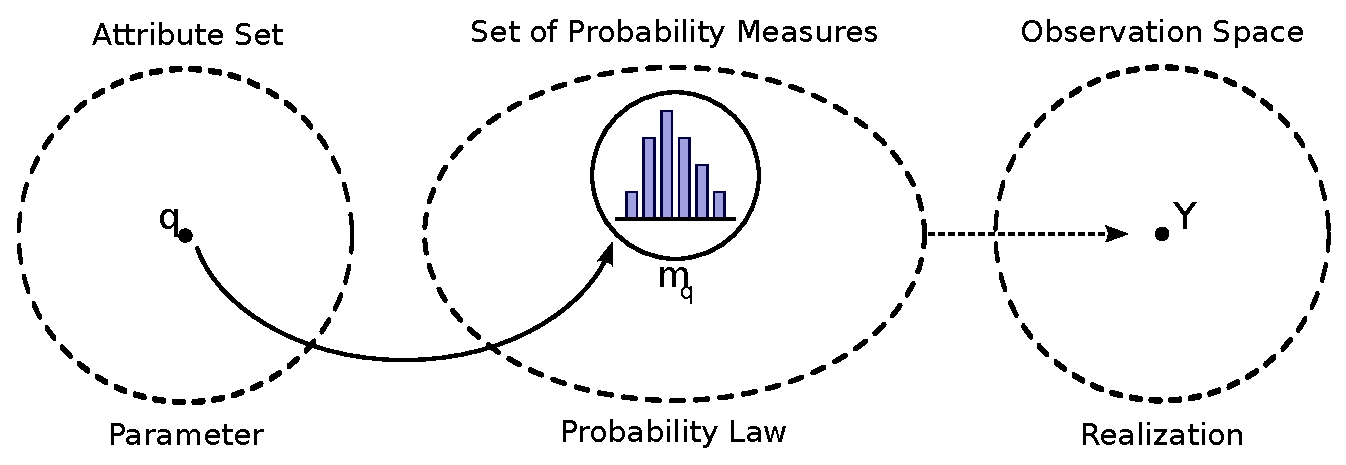
\includegraphics[width=5in]{Figures/1Chapter/Inference}
\end{center}

Three basic components are involved in this framework.
First, there is the \emph{attribute set} which is composed of all admissible values of $\theta$.
This set is represented by $U$.
The second component is a measurable space $(\mathcal{F}, \Omega)$ where $\Omega$ symbolizes the \emph{sample space} and $\mathcal{F}$ is the $\sigma$-algebra of all probability events.
Together, $\mathcal{F}$ and $\Omega$ provides a mathematical basis for the randomness induced by parameter $\theta$.
Finally, the \emph{observation space} $\Gamma$ is the collection of all realizable observations.
One obtains information about the true parameter $\theta$ by observing a random variable $Y$, which maps outcomes from the sample space $\Gamma$ to values in $\Gamma$.

If the attribute set contains a unique element, then the inference problem is trivial and we need not observe $Y$ to determine the value of $\theta$.
The more interesting case, of course, occurs when $U$ contains several distinct elements.
In this situation, the connection between $\theta$ and $Y$ becomes instrumental.
We explore this relationship next.

To each element $\theta \in U$, there corresponds a probability law $\mu_{\theta}$ acting on the measurable space $(\mathcal{F}, \Omega)$.
The true value of $\theta$ thus determines the distribution of random variable $Y$.
While observing the realization of $Y$ may provide information about its distribution, this empirical data is typically insufficient to resolve all the uncertainty surrounding the value of $\theta$.
Statistical signal processing broadly refers to the collection of techniques and methods employed to extract information about the phenomenon of interest from the available data.

\begin{center}
\includegraphics[width=3in]{Figures/1Chapter/StatisticalSignalProcessing}
\end{center}

We provide a simple example below to illustrate how this framework applies to engineering problems.

\begin{example} \label{example:BinaryCommunicationSystem}
A digital communication system transmits a single bit over a noisy channel, using a zero or a one.
The received information is corrupted by additive Gaussian noise, with distribution $\mathcal{N}(0,1)$.
We wish to decide which bit was sent from the received information.
To initiate this process, we cast this problem in the abstract framework described above.
In the present case, the attribute set is $U = \{ 0, 1 \}$; the sample space is the real line; and the corresponding probability density functions are
\begin{equation*}
f_0 (y) = \frac{1}{\sqrt{2 \pi}} e^{- \frac{y^2}{2}} \quad
f_1 (y) = \frac{1}{\sqrt{2 \pi}} e^{- \frac{(y-1)^2}{2}} .
\end{equation*}
Note that in this first example the observation space and the sample space are identical.
\end{example}

The primary characteristics that distinguish statistical inference problems from one another are the amount of a priori knowledge available about the attribute set $U$, the goal underlying the inference procedure, and the performance criterion used to assess the effectiveness of the inference procedure.
If the attribute set is partitioned into a finite or countable number of subsets and the objective is to identify which subset $\theta$ belongs to, then the decision process is termed \emph{detection} or \emph{hypothesis testing}.
In particular, a detector maps every element in the observation space $\Gamma$ to one of the admissible hypotheses.
A graphical interpretation of a detection process is illustrated below.

\begin{center}
\includegraphics[width=3in]{Figures/1Chapter/DetectionModel}
\end{center}

On the other hand, if $U$ contains an uncountable number of candidates and we are tasked with selecting the most appropriate one, then we are facing an \emph{estimation} problem.
In this setting, the goal is to select an estimate $\hat{\theta}$ based on observation $Y$ as to optimize a given objective function.
Thus, parameter estimation is a procedure that takes an argument in observation space $\Gamma$ and returns an element in the attribute set $U$.
The distinction between detection and estimation is at times rhetorical;
we will not delve on this issue.
Rather, our focus will be to develop a solid understanding of statistical signal processing and to become well-versed in applying some of its techniques and algorithms.

A second important distinction among inference problems, as mentioned above, comes from the assumptions made on attribute set $U$.
In \emph{classical estimation}, $U$ is taken to be a specific set containing the unknown parameter $\theta$.
This can be contrasted with the \emph{Bayesian approach} where $U$ is assumed to be a probability space with a specific distribution.
In this latter case, the value of $\theta$ is itself the outcome of a random experiment.
The distinction between these two approaches leads to disparate performance criteria, and hence different estimators.
Such a distinction is also present in detection problems, where the attribute set is either a collection of object with a deterministic parameter $\theta$, or a measurable space with a certain probability law.

A final and less straightforward distinction between inference problems stems from the nature of the empirical observations.
The framework detailed above implicitly assumes that observations can be viewed as random variables.
If on the other hand we have access to empirical data coming from a random process, then the inference problem becomes more challenging.
In this scenario, inference problems are referred to as \emph{signal detection} and \emph{signal estimation}.
When dealing with the progressive estimation of a stochastic process, the statistical inference procedure is often called \emph{filtering}.
We will address some of these problems once we acquire the mathematical sophistication necessary to tackle them.


\section{Modeling Engineering Problems}

These notes present a collection of important tools and methods in statistical signal processing.
Becoming familiar with these tools should provide the reader with the ability to solve various inference problems, and to assess the performance of the corresponding statistical procedures.
Still, an equally important skill to develop is the capacity to take a concrete engineering problem and to formulate it mathematically in a way that leads to a meaningful solution.
In this exposition, we will often use an abstract problem formulation as our starting point.
However, the value of being able to take an engineering challenge and to cast it in a relevant yet solvable framework is not to be understated.
Developing this skill is partly what sets apart the value of one's education and experience.
Throughout, we will provide examples and case studies of meaningful problems together with suitable mathematical interpretations.
Reading there examples carefully and understanding the process of selecting the proper tools to solve them should help develop good intuition.
While going through these notes, one should also try to think about new situations where the statistical methods under consideration apply.



%\section{Organization}
%
%These notes are organized as follows.
%
%In Chapter~\ref{chapter:Detection}, we study hypothesis testing.
%We begin with an introduction to the simplest such problem, binary detection.
%Both the classical and Bayesian forms of the problem are considered.
%The theory of detection is then extended to composite hypothesis testing, a framework where the attribute set contains more than two elements.
%We also discuss the problem of robust detection, sequential detection and quickest change detection.
%Finally, we look at simple instances of $M$-ary hypothesis testing.

%Chapter~\ref{chapter:ClassicalParameterEstimation} is devoted to classical parameter estimation.
%We first introduce the celebrated Cramer-Rao lower bound, which provides a performance limit on unbiased estimators.
%We then present the concept of sufficient statistics.
%This is followed by a discussion of common estimators including the best linear unbiased estimator, the maximum likelihood estimator, and the least squares estimator.
%The expectation-maximization algorithm is also introduced as a numerically tractable estimation methodology.
%
%Chapter~\ref{chapter:BayesianParameterEstimation} presents a study of Bayesian parameter estimation.
%The maximum a posteriori estimator is first introduced.
%This is followed by a discussion of the minimum mean square error and linear minimum mean square error estimators.
%Signal estimation is treated in Chapter~\ref{chapter:SignalEstimation}, where the Kalman-Bucy filter and the Wiener-Kolmogorov filter are introduced.

%estimating the median of a number of integers to which you only have a few observations.




\chapter{Data Compression}

Having explored the process of turning an analog information signal into a digital sequence using sampling and quantization, we begin our treatment of digital information.
From here on, we assume that information sources are digital in nature.
That is, they produce a succession of symbols, each drawn from a \emph{discrete alphabet}.
The two main goals of the current chapter are to find an adequate measure of information for digital systems and to describe compression algorithms that can be employed to represent the said information in a succinct manner.
\emph{Data compression}, also known as \emph{source coding}, is important because it reduces the consumption of expensive resources such as hard disk space or transmission bandwidth.
Alternatively, it can be applied to lower the cost of communication, reduce latency or improve the quality of the received messages.

This document offers an introductory treatment of \emph{lossless compression} algorithms, whereby the original message can be recovered perfectly from the compressed data.
This is in contrast to \emph{lossy data compression}, which can achieve better compression ratio at the expense of introducing some distortion in the message.
In the latter case, part of the information may be lost and the original data need not be perfectly recoverable, although the reconstructed message may be quite close to the original one.
For instance, the JPEG algorithm can be employed as a lossy compression scheme to reduce the size of a digital photograph.
In lossless data compression, two strategies are employed to reduce the expected length of a message.
Highly probable symbols are assigned short descriptions, and less likely symbols are encoded using longer binary representations.
Second, the statistical redundancy contained in the input signal over time is removed, leading to a more concise description of the digital data.
Data compression algorithms are explained more thoroughly below.

As we will see, finding a pertinent measure of information is key in assessing the performance and limitations of compression algorithms.
While the general notion of information may be quite broad, it has a precise definition in the context of digital communication systems.
To describe this specific meaning, we first need to develop a rigorous mathematical model for digital information sources.


\section{Discrete Memoryless Sources}

As mentioned above, a digital source produces a sequence of symbols drawn from a countable alphabet.
It can accordingly be modeled as a discrete-time random process.
Because of their indeterminate nature, random signals and stochastic processes can be quite hard to characterize.
In early sections of this document, we discussed two desirable attributes of random signals, namely stationary and ergodicity.
Yet, we purposely avoided giving an explicit definition for a random process.
A detailed discussion of the subject requires advanced concepts from probability theory, a topic that interested readers may wish to pursue on their own.
For the sake of simplicity, we focus on a class of elementary information sources that are collectively known as discrete memoryless sources.
These sources are easy to analyze and can be described unambiguously in a straightforward manner.
Furthermore, discrete memoryless sources provide valuable insights into the design of efficient compression algorithms for more general settings.

\begin{definition}
A \emph{discrete memoryless source} is a digital information source that produces a sequence of independent and identically distributed symbols over time.
Mathematically, it consists of an alphabet $\mathcal{X}$ and a probability mass function $p_X(\cdot)$ such that, at any time~$t$, the probability that the source outputs symbol $x \in \mathcal{X}$ is equal to $p_X(x)$, irrespective of the past and future.
\end{definition}

For discrete memoryless sources, it suffices to define the probability mass function of individual symbols to completely characterize the statistical properties of the corresponding random signal.
The higher-order statistics need not be specified explicitly, as they can be obtained from
\begin{equation} \label{equation:JointDistributionMemorylessSource}
\Pr (X_{t_1} = x_{t_1}, \ldots, X_{t_n} = x_{t_n})
= \prod_{k = 1}^n p_X(x_{t_k})
\end{equation}
where $x_{t_1}, \ldots, x_{t_n} \in \mathcal{X}$.
In \eqref{equation:JointDistributionMemorylessSource}, the random variable $X_{t_i}$ denotes the output of the source at time~$t_i$.
We provide two examples of memoryless sources below to further illustrate their form.

\begin{example}[Binary Source] \label{example:BinarySource}
The simplest possible information source is a discrete memoryless source where $p_X(\cdot)$ is the probability mass function of a Bernoulli random variable,
\begin{equation*}
p_X(x) = \begin{cases} (1 - p), & x = 0 \\
p, & x = 1 \end{cases}
\end{equation*}
with $p \in [0,1]$.
This source can be employed, for instance, to model the successive flipping of a biased coin, where heads is obtained with probability $p$ and tails is obtained with probability $1 - p$.
\end{example}

\begin{example}
To construct a slightly more elaborate example, consider a collection of experiments where a fair coin is flipped repetitively until heads is observed.
The outcome of each experiment is reported as a source output.
The source alphabet in this case is $\mathcal{X} = \{1, 2, \ldots \}$, the positive integers, and the marginal probability mass function associated with individual outcomes becomes
\begin{equation*}
p_X (x) = \frac{1}{2^x}, \quad x = 1, 2, \ldots
\end{equation*}
Thus, the distribution of the source output at time~$t$ is a geometric random variable with parameter~$\frac{1}{2}$.
\end{example}

It is straightforward to show that all discrete memoryless sources are both stationary and ergodic.
The fact that their outcomes are independent over time makes them convenient for analysis, leading to simple interpretations.
However, it should also be pointed out that many realistic sources are more complicated than memoryless sources.
In particular, their outputs may be correlated over time, which can have a major impact on information rates.
Handling intricate sources requires heavy mathematical machinery, and is beyond the scope of this document.
The results derived using more involved sources are, nevertheless, similar in nature to the ones presented below.
This partially explains why we choose not to study more difficult information sources in this document.

Having constructed a suitable abstraction for digital sources, we turn to the subject of digital information.
From an intuitive point of view, the data rate of a discrete memoryless source should be equal to the amount of information it produces at every time instant.
In other words, the amount of information created by a discrete memoryless source at time~$t$ should be computable based on $\mathcal{X}$ and $p_X(\cdot)$ exclusively.
This is indeed the case.
Before we can make this statement precise, we need a rigorous mathematical characterization of information.
We address this issue by introducing entropy, a concept closely related to the notion of information.


\section{Entropy}

The \emph{entropy} can be viewed as a measure of uncertainty in a random variable.
In the context of digital communications, it serves as a measure of information in that it provides a lower bound on the expected number of bits required to describe the output of a discrete memoryless source.
This lower bound is tight and can be approached using various schemes, as we will see shortly.

\begin{definition}[Entropy]
Let $X$ be a discrete random variable drawn from alphabet $\mathcal{X}$ according to probability mass function $p_X(\cdot)$.
The entropy of $X$, denoted $\mathrm{H}[X]$, is given by
\begin{equation} \label{equation:Entropy}
\mathrm{H}[X] = - \sum_{x \in \mathcal{X}} p_X (x) \log_2 ( p_X(x) ) .
\end{equation}
Under this definition, entropy is described in bits.
When writing $\mathrm{H}[X]$, we use the convention
\begin{equation*}
0 \cdot \log_2 \left( \frac{1}{0} \right)
= \lim_{\epsilon \rightarrow 0} \epsilon \log_2 \left( \frac{1}{\epsilon} \right)
= 0 .
\end{equation*}
Alternatively, the entropy of $X$ can be interpreted as the expectation of a logarithmic function,
\begin{equation*}
\mathrm{H}[X] = \mathrm{E} \left[ \log_2 \left( \frac{1}{p_X(X)} \right) \right] .
\end{equation*}
\end{definition}

The entropy as described in \eqref{equation:Entropy} has interesting properties.
The value $\mathrm{H}[X]$ does not depend on the actual symbols themselves, it only depends on the probability mass function of the possible outcomes.
For instance, in Example~\ref{example:EntropyFairCoin}, the entropy of $X$ remains the same whether we represent the flipping of a coin by a single bit or through a string of letters, heads or tails.
More generally, the way we choose to designate the possible outcomes of a random experiment has no bearing over the entropy of the corresponding source, only the respective probabilities of the possible symbols matter.

\begin{example} \label{example:EntropyFairCoin}
Let $X$ be an abstract representation of the flipping of a (possibly biased) coin.
The probability mass function of $X$ is then equal to
\begin{equation*}
p_X(x) = \begin{cases} (1-p), & x = 0 \\
p, & x = 1 \end{cases}
\end{equation*}
with zero denoting tails and one for heads.
We can compute the entropy of $X$ as follows,
\begin{equation*}
\mathrm{H}[X] = - (1-p) \log_2 (1-p)
- p \log_2 (p) .
\end{equation*}
If the coin is fair, $p = \frac{1}{2}$, then the entropy of $X$ becomes one  bit.
Hence, the minimum expected number of bits needed to describe the outcome of a fair coin toss is one.
This seems quite reasonable.
\end{example}

%
% plot of binary entorpy needed.
%

The entropy of pair of two independent random variables is the sum of the individual entropies.
Suppose that $X$ is a vector random variable given by $X = (U, V)$, where $U$ and $V$ are independent.
Then, we can write
\begin{equation*}
p_X(x) = p_X((u, v)) = p_{U} (u) p_{V} (v)
\end{equation*}
and the entropy of $X$ can be computed as
\begin{equation*}
\begin{split}
\mathrm{H}[X] &= - \sum_{ x \in \mathcal{X} } p_X(x) \log_2 ( p_X(x) ) \\
&= - \sum_{(u, v) \in \mathcal{U} \times \mathcal{V}}
p_X((u, v)) \log_2 ( p_X((u, v)) ) \\
&= - \sum_{u \in \mathcal{U}} \sum_{v \in \mathcal{V}}
p_{U} (u) p_{V} (v) \log_2 ( p_{U} (u) p_{V} (v) ) \\
&= - \sum_{u \in \mathcal{U}}
p_{U} (u) \log_2 ( p_{U} (u) )
- \sum_{v \in \mathcal{V}}
p_{V} (v) \log_2 ( p_{V} (v) ) \\
&= \mathrm{H}[U] + \mathrm{H}[V] .
\end{split}
\end{equation*}
This corresponds to our intuitive understanding; the amount of information contained in two unrelated events should be the sum of the information pertaining to each individual event.

It is important to recognize that $\mathrm{H}[X]$ is computed based on the probability mass function $p_X(\cdot)$, it is not a function of the random variable $X$ itself.
As such, $\mathrm{H}[X]$ is a deterministic quantity and does not depend on the actual realization of $X$.
Furthermore, we note that $\mathrm{H}[X]$ is continuous in the weights of the distribution $p_X(\cdot)$.
A small change in the distribution of $X$ only results in a small variation in its entropy.
It is therefore possible to construct accurate entropy estimates based on empirical measurements of the source outputs.


\section{Variable-Length Compression Codes}

A \emph{code} is a rule for converting a symbol (or a group of symbols) into a string of bits called a \emph{codeword}.
Mathematically, an encoder is a mapping $c : \mathcal{X} \mapsto \mathcal{C}$ from the input alphabet $\mathcal{X}$ to the collection of possible codewords $\mathcal{C}$.
The goal of a \emph{compression code} is, of course, to provide a more concise representation of the information signal.
In lossless compression, the function $c$ must be injective over the support of $X$.
Without this one-to-one relationship, decoding errors are bound to happen.
Encoding schemes can be partitioned into two categories based on the structure of their codebooks.
If the codewords all share the same bit-length, then the corresponding code is called a \emph{fixed-length code}.
This section focuses on codes in the second category, variable-length codes, which are often used in lossless data compression.

As the name suggests, a \emph{variable-length code} is an encoding function that maps source symbols to a variable number of bits.
This is a beneficial feature for many compression schemes, as the greater flexibility sometimes leads to better compression ratio.
The motivation behind variable-length encoding is the intuition that data compression can be achieved by assigning short bit strings to likely symbols, and necessarily longer bit strings to less probable ones.
In dealing with variable-length codes, it is essential to recognize that they are inherently more tricky than fixed-length ones.
With variable-length coding, it may be impossible to know where codewords begin in a compressed binary file without knowing the content of the file.
This is in stark contrast with fixed-length codes where codewords are positioned at regular intervals and, therefore, easy to distinguish.
To ensure that the binary output of a variable-length encoder can be recovered unambiguously, the code needs specific properties.

Variable-length codes can be nested in order of decreasing generality as non-singular, uniquely decodable and instantaneous.
A code is \emph{non-singular} if each source symbol is mapped to a different bit string.
That is, the mapping $c$ from $\mathcal{X}$ to $\mathcal{C}$ is one-to-one.
Rather, if two symbols map to the same codeword, then it is intuitively clear that the original message cannot be recovered with certainty.
A code is said to be \emph{uniquely decodable} if its extensions are non-singular.
The extension of a code $c$ is obtained by concatenating its codewords when $c$ is applied to a multitude of source symbols.
Given the string of symbols $x_1, x_2, \ldots, x_n$, the extension of $c$ produces the output bit string
\begin{equation*}
c(x_1) c(x_2) \cdots c(x_n) .
\end{equation*}
An extension of $c$ is a proper encoding schemes because it takes a group of symbols as its argument and produces a string of bits as its output.

It is important to recognize that successive codewords in a message are communicated as an undifferentiated sequence of bits.
There is no separation marker or frame between adjacent codewords, no commas or spaces.
The decoder, given a starting point, must infer the boundaries of every codeword from the data.
This process is called \emph{parsing}.
The third and final property of variable-length encoding is related to parsing.
A code is \emph{instantaneous}, or \emph{prefix-free}, if no codeword in $\mathcal{C}$ is a prefix of a any other encoded symbol in $\mathcal{C}$.
This property guarantees that each encoded symbol can be identified with no further delay once the corresponding string of bits is received or read.

\begin{example}
Suppose that a source produces three possible symbols, $\mathcal{X} = \{ x_1, x_2, x_3 \}$.
We consider four encoding functions ($c_1, c_2, c_3, c_4$), each with different properties.
The encoding schemes are defined as follows.

\begin{center}
\begin{tabular}{|c|c|c|c|c|}
\hline
Symbol & \multicolumn{4}{c|}{Codeword} \\
\hline
$x$ & $c_1(x)$ & $c_2(x)$ & $c_3(x)$ & $c_4(x)$ \\
\hline
$x_1$ & 0 & 0 & 0 & 0 \\
$x_2$ & 1 & 1 & 01 & 10 \\
$x_3$ & 0 & 01 & 11 & 11 \\
\hline
\end{tabular}
\end{center}

The first scheme is not injective because it maps two different source symbols to the same codeword, $c_1(x_1) = c_1(x_3)$.
Thus, individual codewords cannot be decoded unambiguously.
The second code is one-to-one; however, it is not uniquely decodable.
The encoded message 01 can be generated by either input string $x_1 x_2$ or input symbol $x_3$.
Clearly, the compressed message is not uniquely decodable.
The third code, $c_3(\cdot)$ is uniquely decodable, but not instantaneous.
After receiving a zero, it not immediately clear whether $x_1$ produced this output or if this zero consists of the first half of codeword $c(x_2)$.
While $c_4(\cdot)$ is a prefix code where every symbol can be decoded immediately after reading the corresponding bits.
\end{example}

The measure of a good prefix code is the expected length of its encoded symbols.
Suppose that a discrete memoryless source $(\mathcal{X}, p_X)$ is given along with a code $c$.
We denote the length in bits of codeword $c(x)$ by $\ell_c(x)$.
The expected number of bits produced by the source at each time instant is given by
\begin{equation} \label{equation:CodeRateCompression}
\mathrm{E} [ \ell_c (X) ] = \sum_{x \in \mathcal{X}} p_X(x) \ell_c(x) .
\end{equation}
We emphasize that the expected length is a function of both the statistics of the source and the structure of compression code employed.
Under the assumption that the source outcomes are independent and identically distributed over time, $\mathrm{E} [ \ell_c (X)]$ also represents the average data rate produced by the source, in bits per source symbol.


\subsection{Kraft Inequality}

When building a compression code, it is obvious from \eqref{equation:CodeRateCompression} that assigning short codewords is better than long codewords.
Yet, it is clear that we cannot describe every symbol using a very small number of bits, for otherwise the prefix condition will be violated.
The collection of possible length assignments for a prefix-free code is characterized by the following inequality.

\begin{theorem}[Kraft Inequality]
Let $\mathcal{X}$ be a finite alphabet.
Any binary prefix-free code $c : \mathcal{X} \mapsto \mathcal{C}$ satisfies the inequality
\begin{equation} \label{equation:KraftInequality}
\sum_{x \in \mathcal{X}} 2^{-\ell_c(x)} \leq 1.
\end{equation}
where $\ell_c(x)$ is the bit length of codeword $c(x)$.
Conversely, if we first assign the codeword lengths such that \eqref{equation:KraftInequality} is satisfied, then there exists an instantaneous code with these codeword lengths.
\end{theorem}
\begin{proof}
We wish to give necessary and sufficient conditions about the existence of a prefix-free code with a specific length assignment.
We employ simple combinatorial arguments to a binary tree structure to establish this result.
\begin{figure}[htbp]
\begin{center}
\begin{psfrags}
\psfrag{0}[c]{$0$}
\psfrag{1}[c]{$1$}
\psfrag{C0}[l]{$000$}
\psfrag{C1}[l]{$001$}
\psfrag{C2}[l]{$010$}
\psfrag{C3}[l]{$011$}
\psfrag{C4}[l]{$100$}
\psfrag{C5}[l]{$101$}
\psfrag{C6}[l]{$110$}
\psfrag{C7}[l]{$111$}
\epsfig{file=Figures/binarytree,width=7cm}
\end{psfrags}
\caption{This figure shows a binary tree with depth $L_c = 3$ and eight leaves.  The branches from every node correspond to zero or one.}
\label{figure:BinaryTree}
\end{center}
\end{figure}
Let $L_c = \max_{x \in \mathcal{X}} \ell_c (x)$ be the length of the longest codeword.
Code $c: \mathcal{X} \mapsto \mathcal{C}$ can be defined using a binary tree of depth $L_c$, where branches from every node correspond either to zero or one.
Each codeword consists of a unique path from the root to a leaf at depth $\ell_c(x)$, following its binary string expansion.
The prefix condition ensures that no codeword is a descendant of any other codeword in the binary tree.
For the codewords in the tree, let $S_x$ be the set of descendants that $c(x)$ would have in a full binary tree of depth $L_c$.
The sets $S_x$ are disjoint because of the prefix-free nature of the code, and $|S_x| = 2^{L_c - \ell_c(x)}$.
Since the total number of nodes at depth $L_c$ is $2^{L_c}$, we have
\begin{equation*}
\left| \bigcup_{x \in \mathcal{X}} S_x \right|
= \sum_{x \in \mathcal{X}} |S_x|
= \sum_{x \in \mathcal{X}} 2^{L_c - \ell_c(x)}
\leq 2^{L_c} .
\end{equation*}
By dividing both sides by $2^{L_c}$, we conclude that \eqref{equation:KraftInequality} holds.
That is, a binary prefix-free code $c$ over finite alphabet $\mathcal{X}$ satisfies the Kraft inequality.

Conversely, suppose that we have a code assignment such that \eqref{equation:KraftInequality} is satisfied.
Without loss of generality, we assume that the codeword lengths $\ell_c(x_i)$ are increasing in~$i$,
\begin{equation*}
\ell_c(x_1) \leq \ell_c(x_2) \leq \ell_c(x_3) \leq \cdots
\end{equation*}
We can construct a prefix code with matching codeword lengths by pruning subtrees from a  full binary tree of depth $L_c$.
First, choose any node from the full tree at depth $\ell_1$ and remove all of its descendants.
This removes $2^{L_c -\ell_1}$ leafs from the original binary tree.
Next, select any available node from the resulting tree at depth $\ell_2$, and remove all of its descendants.
This time, an additional $2^{L_c - \ell_2}$ leafs are taken away from the original binary tree.
Continue this procedure with the other codeword lengths.
After $m$ iterations, the total number of leafs removed from the original binary tree is equal to
\begin{equation*}
\sum_{i=1}^m 2^{L_c - \ell_i} = 2^{L_c} \sum_{i=1}^m 2^{-\ell_i} .
\end{equation*}
Since the Kraft inequality holds for the codeword length assignment, this implies that all the codewords can be placed at different positions on the binary graph.
Then, following the binary structure of the graph, the binary string of the codes can be inferred from the graph.
\end{proof}

\begin{example}[Code on a Tree]
Suppose that we intend to construct a prefix code for $\mathcal{X} = \{ x_1, \ldots, x_5 \}$, with code lengths
\begin{xalignat*}{3}
\ell_c(x_1) &= \ell_c(x_2) = 2 & \ell_c(x_3) &= \ell_c(x_4) = 3 & \ell_c(x_5) &= 2.
\end{xalignat*}
First, we check the Kraft inequality to make sure that such an assignment is feasible,
\begin{equation*}
\sum_{i = 1}^5 2^{-\ell_c(x_1)}
= \frac{1}{4} + \frac{1}{4} + \frac{1}{8} + \frac{1}{8} + \frac{1}{4} = 1 .
\end{equation*}
The inequality is fulfilled, we can therefore use a binary tree construction to design the desired instantaneous code.
The process is illustrated in Figure~\ref{figure:BinaryTreeCode}, and the resulting code is shown below.

\begin{center}
\begin{tabular}{|c|c|c|c|}
\hline
Source Symbol & Codeword & Source Symbol & Codeword \\
\hline
$x_1$ & 00 & $x_4$ & 101 \\
$x_2$ & 01 & $x_5$ & 11 \\
$x_3$ & 100 & & \\
\hline
\end{tabular}
\end{center}

Since the Kraft inequality is met with equality, we know that it is impossible to get a better code by shortening one of the codewords.
\begin{figure}[htbp]
\begin{center}
\begin{psfrags}
\psfrag{0}[c]{$0$}
\psfrag{1}[c]{$1$}
\psfrag{00}[l]{$00$}
\psfrag{01}[l]{$01$}
\psfrag{100}[l]{$100$}
\psfrag{101}[l]{$101$}
\psfrag{11}[l]{$11$}
\epsfig{file=Figures/binarytreecode,width=7cm}
\end{psfrags}
\caption{Construction of a prefix code with a binary tree.}
\label{figure:BinaryTreeCode}
\end{center}
\end{figure}
\end{example}


\subsection{Entropy Bounds on Prefix-Free Codes}

Now that we know how to build instantaneous, we consider the problem of finding good prefix-free codes.
Recall from \eqref{equation:CodeRateCompression} that our objective is to find a prefix-free code with the smallest possible expected length.
As seen earlier, this codeword length assignment is subject to the Kraft inequality.
Putting these two requirements together, we can formulate the optimization problem as follows,
\begin{equation*}
\min_{\ell(x)} \sum_{x \in \mathcal{X}} p_X(x) \ell(x)
\quad \text{subject to} \quad
\sum_{x \in \mathcal{X}} 2^{- \ell(x)} \leq 1 .
\end{equation*}
We note that, for a code to exist, the function $\ell(x)$ must take values in the positive integers.
It turns out that this problem is difficult to solve.

To gain insight into the problem, we relax the integer constrain on $\ell(x)$.
This added flexibility will provide a lower bound on $\mathrm{E} [\ell(X)]$; having more choices can only lead to better results.
We use the method of Lagrange multipliers to solve the latter version of the problem.
The objective function, with Lagrange multiplier $\lambda$, becomes
\begin{equation*}
\sum_{x \in \mathcal{X}} p_X(x) \ell(x)
+ \lambda \left( \sum_{x \in \mathcal{X}} 2^{- \ell(x)} - 1 \right) .
\end{equation*}
Note that this function is twice differentiable in $\ell(x)$.
Taking a partial derivative with respect to $\ell(x)$ and setting it to zero, we get
\begin{equation*}
p_X(x) - \lambda \ln(2) 2^{- \ell(x)}  = 0 .
\end{equation*}
The optimal value for $\ell(x)$, which we denote by $\ell^{\star}(x)$, must therefore satisfy $2^{- \ell^{\star}(x)} = p_X(x) / (\lambda \ln (2))$.
Computing the derivative with respect to $\lambda$ yields
\begin{equation*}
\sum_{x \in \mathcal{X}} 2^{- \ell^{\star}(x)} = 1 ,
\end{equation*}
which in turn implies $\lambda = 1 / \ln (2)$.
Putting these results together, we gather that the optimal values for $\{ \ell(x) : x \in \mathcal{X} \}$ are given by
\begin{equation*}
\ell^{\star}(x) = - \log_2 (p_X(x))
\end{equation*}
for $x \in \mathcal{X}$.
Thus, by construction, we obtain
\begin{equation*}
\mathrm{E} [\ell_c(X)] \geq - \sum_{x \in \mathcal{X}} p_X(x) \log_2 (p_X(x))
= \mathrm{H}[X]
\end{equation*}
for any prefix-code~$c$.
In other words, the entropy is a lower bound on the expected length of any prefix-free code.

It is equally easy to obtain an upper bound on the expected length of an optimal prefix-free code.
Observe that $\lceil - \log_2 (p_X(x)) \rceil$ is an integer, with
\begin{equation*}
- \log_2 (p_X(x))
\leq \lceil - \log_2 (p_X(x)) \rceil
\leq - \log_2 (p_X(x)) + 1 .
\end{equation*}
The Kraft inequality asserts that we can build a code $c : \mathcal{X} \mapsto \mathcal{C}$ such that $\ell_c(x) = \lceil - \log_2 (p_X(x)) \rceil$, as
\begin{equation*}
\sum_{x \in \mathcal{X}} 2^{- \ell_c(x)}
\leq \sum_{x \in \mathcal{X}} 2^{- \ell^{\star}(x)} = 1 .
\end{equation*}
As such, there exists a code~$c$ such that
\begin{equation*}
\mathrm{E} [\ell_c(X)] \leq \mathrm{H}[X] + 1 .
\end{equation*}
We collect and formalize these important results in the form of a theorem.

\begin{theorem} \label{theorem:EntropyBoundsPrefixCodes}
Consider a discrete memoryless source $(\mathcal{X}, p_X(\cdot))$ over a finite alphabet.
If symbols are encoded individually using an optimal prefix-free code $c : \mathcal{X} \mapsto \mathcal{C}$, then the expected length of the codewords satisfies
\begin{equation*}
\mathrm{H}[X] \leq \mathrm{E} [\ell_c(X)] \leq \mathrm{H}[X] + 1 .
\end{equation*}
\end{theorem}


\subsection{Huffman Codes}

Theorem~\ref{theorem:EntropyBoundsPrefixCodes} identifies properties of an optimal prefix-code.
However, it does not provide an algorithmic methodology to design such a code.
This is addressed by the \emph{Huffman encoding algorithm}, a technique that produces an efficient variable-length code for lossless data compression.
Not too surprisingly, the underlying strategy in this scheme is to assign short strings of bits to likely symbols, and necessarily longer ones to less probable source outputs.
The encoding is specifically crafted so that the code table forms a prefix-free code.
Huffman codes are the most efficient compression mapping for individual source symbols.
The expected length of the compressed data achieved with this technique will be no greater than the expected message length of any other prefix-free code that operates on individual source symbols.

The insight behind Huffman coding is based on three properties of optimal prefix-codes.
Suppose that we wish to encode outputs from discrete memoryless source $(\mathcal{X}, p_X)$, and let $c^{\star} : \mathcal{X} \mapsto \mathcal{C}$ be an optimal prefix-code for this source.
If $p_X(x_1) > p_X(x_2)$, then $\ell_{c^{\star}}(x_1) \leq \ell_{c^{\star}}(x_2)$.
For any of the longest codewords, its sibling (the bit string that differs only in the last digit) must also be codeword; otherwise, the original codeword can be shortened by removing the last bit.
Finally, the code tree associated with an optimal code must be full.
A binary tree is \emph{full} if every node has either zero or two children.
Again, if this condition fails, then some codewords in the codebook can be shortened.

The Huffman algorithm creates a code by building a binary tree.
The algorithm proceeds as follows.
First, every source symbol $x$ is assigned to an individual node.
Then, the simple recursion outlined below is applied.
\begin{enumerate}
\item Sort the nodes in decreasing order of probabilities.
\item Merge the two least probable nodes into a single one, whose probability equals the sum of its constituents.
\item Arbitrarily assign zero or one to the branches emerging from this new node.
\item Repeat the previous three steps with the new collection of nodes and their corresponding probabilities until only one node remains.
\end{enumerate}
The Huffman encoding algorithm is best grasped through simple examples.

\begin{example}
Suppose that a discrete memoryless source $(\mathcal{X}, p_X)$ with alphabet $\mathcal{X} = \{ x_1, x_2, x_3 \}$ has probability mass function
\begin{equation*}
p_X(x) = \begin{cases} \frac{2}{3}, & x = x_1 \\
\frac{1}{6}, & x \in \{ x_2, x_3 \} . \end{cases}
\end{equation*}
We wish to obtain an optimal prefix-code for this source, and thus we apply the Huffman algorithm.
For the given source, code design proceeds as follows.

\begin{center}
\begin{tabular}{|c|c|c|c|c|}
\hline
Stage 3 & Stage 2 & Stage 1 & Symbol & Codeword \\
\hline
$\Pr \{ x_1, x_2, x_3 \} = 1$ & $\Pr \{ x_1 \} = \frac{2}{3}$
& $p_X (x_1) = \frac{2}{3}$ & $x_1$ & 0 \\
& $\Pr \{ x_2, x_3 \} = \frac{1}{3}$ & $p_X (x_2) = \frac{1}{6}$ & $x_2$ & 10 \\
& & $p_X (x_3) = \frac{1}{6}$ & $x_3$ & 11 \\
\hline
\end{tabular}
\end{center}

From this successive re-ordering of probabilities, we use a binary tree to build the actual code.
This is illustrated in Figure~\ref{figure:Huffman1}.
\begin{figure}[htbp]
\begin{center}
\begin{psfrags}
\psfrag{C1}[l]{$0$}
\psfrag{C2}[l]{$10$}
\psfrag{C3}[l]{$11$}
\psfrag{x1}[c]{$x_1$}
\psfrag{x2}[c]{$x_2$}
\psfrag{x3}[c]{$x_3$}
\psfrag{x23}[c]{$\{ x_2, x_3 \}$}
\psfrag{x123}[c]{$\{ x_1, x_2, x_3 \}$}
\epsfig{file=Figures/huffman1,width=68.718mm}
\end{psfrags}
\caption{A graphical representation for the construction of a simple Huffman code. The source alphabet in this case is $\mathcal{X} = \{x_1, x_2, x_3 \}$ and the probabilities of individual symbols are $\{ 2/3, 1/6, 1/6 \}$, respectively.}
\label{figure:Huffman1}
\end{center}
\end{figure}
\end{example}

\begin{example}
A source $(\mathcal{Y}, p_Y)$ generates four different symbols $\{ y_1, y_2, y_3, y_4 \}$ with probabilities $\{ 0.35, 0.25, 0.2, 0.2 \}$.
A binary tree is generated from right to left, by merging the two less probable symbols at every step.
Once this is complete, the code can then be form by assigning different bits to every pair of branches emerging from a node.
The table below shows the different stages of the iterative procedure where probabilities are first sorted in decreasing order, then the two least probable nodes are merged into a single one.

\begin{center}
\begin{tabular}{|c|c|c|c|}
\hline
Stage 4 & Stage 3 & Stage 2 & Stage 1 \\
\hline
$0.6 + 0.4 = 1$ & $0.35 + 0.25 = 0.6$ & $0.2 + 0.2 = 0.4$ & $p_X (x_1) = 0.35$ \\
& $0.4$ & $0.35$ & $p_X (x_2) = 0.25$ \\
& & $0.25$ & $p_X (x_3) = 0.2$ \\
& & & $p_X (x_4) = 0.2$ \\
\hline
\end{tabular}
\end{center}

The ensuing Huffman code is obtained by moving from left to right in the corresponding binary tree.
The binary tree and the resulting Huffman code are shown in Figure~\ref{figure:Huffman2}.

\begin{figure}[htbp]
\begin{center}
\begin{psfrags}
\psfrag{C1}[l]{$00$}
\psfrag{C2}[l]{$01$}
\psfrag{C3}[l]{$10$}
\psfrag{C4}[l]{$11$}
\psfrag{x1}[c]{$x_1$}
\psfrag{x2}[c]{$x_2$}
\psfrag{x3}[c]{$x_3$}
\psfrag{x4}[c]{$x_4$}
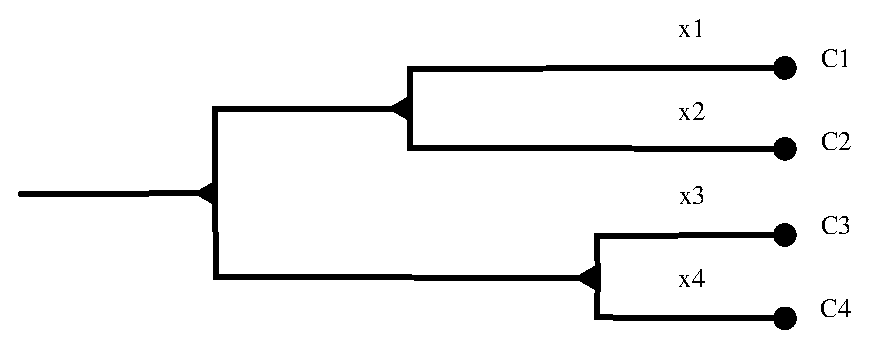
\epsfig{file=Figures/huffman2,width=87.791mm}
\end{psfrags}
\caption{This figure depcits a Huffman code construction for an alphabet of size four.}
\label{figure:Huffman2}
\end{center}
\end{figure}

\end{example}

Although Huffman coding is optimal for a symbol-by-symbol encoding with a known input probability mass function, it can be outperformed when these two conditions are not known.
For instance, if the input distribution $p_X(\cdot)$ is not known, then it must be inferred from the available data prior to applying Huffman coding.
Small errors in the estimated probability mass function can then lead to inefficiency, which in turn renders Huffman coding suboptimal.
We will soon see an encoding algorithm that does not require the input distribution $p_X(\cdot)$.
However, before we can present this algorithm, we need to consider the join encoding of source symbols.


\section{Joint Encoding of Source Symbols}

Under special circumstances, namely when the probability of every source symbol is an exponent base two, the expected length of a Huffman code is equal to the entropy of the source.
However, in many situations, this is not the case, and there exists a gap between the expected codeword length and the entropy of a source output.
An efficient way to encode data, where the expected number of coded bits per source symbol approaches the entropy, is to consider blocks of source symbols and to encode them jointly.
Although more complicated, this process leads to better performance and typically leads to expected message lengths that are shorter  than that of a symbol-by-symbol Huffman code.

Consider a sequence $X_1, X_2, \ldots$ of symbols at the output of a discrete memoryless source.
Instead of using a code that operates on individual symbols, we can design a more elaborate code that takes as input a group of $n$ symbols, $c: \mathcal{X}^n \mapsto \mathcal{C}$.
Since the outputs of a discrete memoryless source are independent and identically distributed random variables, we know from the additive property of the entropy that
\begin{equation*}
\mathrm{H}[X_1, \ldots, X_n ] = n \mathrm{H} [X] .
\end{equation*}
Then, by applying Theorem~\ref{theorem:EntropyBoundsPrefixCodes}, we get that an optimal prefix code, which operates on $\mathcal{X}^n$, yields
\begin{equation*}
n \mathrm{H}[X] \leq \mathrm{E} [ \ell_c (X_1, \ldots, X_n) ] \leq n \mathrm{H}[X] + 1.
\end{equation*}
Then, the expected message length per source output becomes
\begin{equation*}
\mathrm{H}[X] \leq \frac{ \mathrm{E} [ \ell_c (X_1, \ldots, X_n) ] }{n} \leq \mathrm{H}[X] + \frac{1}{n} .
\end{equation*}
Thus, the expected number of bits per symbol produced by a source can be made arbitrarily close to $\mathrm{H}[X]$ by jointly encoding strings of symbols.

\begin{example} \label{example:JointSourceCoding}
Let $(\mathcal{X}, p_X)$ be a binary discrete memoryless source, as described in Example~\ref{example:BinarySource}.
Furthermore, assume that Bernoulli parameter $p$ is equal to $\frac{1}{4}$.
Then, the entropy of the source can be calculated as
\begin{equation*}
\mathrm{H}[X] = - \frac{3}{4} \log_2 \left( \frac{3}{4} \right)
- \frac{1}{4} \log_2 \left( \frac{1}{4} \right)
\approx 0.811 .
\end{equation*}
Since there are only two source symbols, a code generated by the Huffman algorithm is the identity code, where a source output is represented by its binary value.
In this case, the expected codeword length is equal to one.

Suppose instead that two symbols are encoded at a time.
In this case, the possible inputs to the encoder are $\{ 00, 01, 10, 11 \}$, with respective probabilities $\left\{ \frac{9}{16}, \frac{3}{16}, \frac{3}{16}, \frac{1}{16} \right\}$.
The Huffman code specified by
\begin{center}
\begin{tabular}{|c|c|c|c|c|}
\hline
Symbol & Codeword \\
\hline
$00$ & 0 \\
$01$ & 10 \\
$10$ & 110 \\
$11$ & 111 \\
\hline
\end{tabular}
\end{center}
has an expected length of
\begin{equation*}
\mathrm{E} [\ell_c (X_1, X_2)] = 1 \cdot \frac{9}{16} + 2 \cdot \frac{3}{16}
+ 3 \cdot \frac{3}{16} + 3 \cdot \frac{1}{16}
= \frac{27}{16} . 
\end{equation*}
The expected message length per source output becomes
\begin{equation*}
\frac{\mathrm{E} [\ell_c (X_1, X_2)]}{2} = \frac{27}{32} \approx 0.844 ,
\end{equation*}
which is much closer to the entropy of individual source symbols.
Repeating this procedure with an Huffman code that takes three symbols as its input would lead to an expected codeword length per symbol of approximately $0.823$.
\end{example}

Example~\ref{example:JointSourceCoding} illustrates well how encoding several source symbol at a time can lead to a decrease in the expected codeword length per symbol.
The joint encoding of source symbols works even better for sources that are correlated over time.
Although we will not discuss the specificities of this scenario, it is informative to mention that joint source coding is instrumental in approaching the entropy rate of correlated sources.
This is especially important considering the fact that symbol-by-symbol encoding may perform very poorly for correlated sources.


\section{Fixed-Length Compression Codes}

In the previous section, the joint encoding of multiple source symbols was shown to perform well, with the average number of bits per symbol produced by a source approaching $\mathrm{H}[X]$.
Below, we explore how the joint encoding of symbols together with fixed-length codes can be used to produce good compression ratios.
Fixed-length compression codes have several advantages.
They are simple to encode and easy to decode, yielding unambiguous messages.
Furthermore, all fixed-length codes are prefix-free, and encoded symbols can therefore be recovered instantaneously.
However, fixed-length codes cannot be used to compress data by assigning short descriptions to most frequent symbols and longer descriptions to the less likely ones.
Data compression in fixed-length coding methods is only possible for large blocks of data, and any compression beyond the logarithm of the total number of possibilities comes with a finite, though perhaps small, probability of decoding failure.

The minimum number of binary strings in lossless fixed-length symbol-by-symbol encoding is $\left\lceil \log_2 ( | \mathcal{X} | ) \right\rceil$, where $| \mathcal{X} |$ is the size of the source alphabet and $\lceil \cdot \rceil$ is the ceiling function, which returns the smallest integer greater than or equal to its argument.
More generally, the minimum number of binary strings necessary to encode a group of $n$ symbols is $\left\lceil n \log_2 ( | \mathcal{X} | ) \right\rceil$.
This strategy alone, encoding multiple source symbols at a time, is not powerful enough to compress data using fixed-length codes.
To design effective fixed-length codes, two components are necessary.
First, we need to relax the assumption that the data compression scheme should be lossless, rather we allow a small probability of encoding failure.
In particular, we assume that the probability of encoding failure, where data cannot be decoded properly, is $\delta > 0$, where $\delta$ is implicitly very small.
The second ingredient to fixed-length compression is the \emph{asymptotic equipartition property}, which we review next.


\subsection{Asymptotic Equipartition Property}

The AEP is a general property of the output samples of discrete memoryless sources.
This property implies that, given a very long sequence of $n$ source symbols, the probability that $(X_1, \ldots, X_n)$ belongs to a set of typical sample strings is almost one.
It takes a few steps to make this statement precise.

\begin{theorem} \label{theorem:WeakLawEntropy}
Let $(\mathcal{X}, p_X)$ be a discrete memoryless source, which produces a sequence of symbols $X_1, X_2, \ldots $
Furthermore, assume that the output alphabet $\mathcal{X}$ is finite.
The asymptotic equipartition probability asserts that
\begin{equation*}
\lim_{n \rightarrow \infty} - \frac{1}{n} \log_2 \left( p_{X^n} (X_1, \ldots X_n) \right)
= \mathrm{H} [X] .
\end{equation*}
\end{theorem}
\begin{proof}
We can proof this theorem through an application of the weak law of large numbers.
First, we observe that
\begin{equation*}
\begin{split}
\log_2 \left( p_{X^n} (X_1, \ldots X_n) \right)
&= \log_2 \left( \prod_{k=1}^n p_{X} (X_k) \right) \\
&= \sum_{k=1}^n \log_2 p_{X} (X_k) .
\end{split}
\end{equation*}
That is, $\log_2 \left( p_{X^n} (X_1, \ldots X_n) \right)$ is a sum of independent and identically distributed random variables, with bounded second moment.
It follows, by the law of large numbers, that
\begin{equation*}
- \frac{1}{n} \log_2 \left( p_{X^n} (X_1, \ldots X_n) \right)
\end{equation*}
converges in probability to $\mathrm{E} \left[ - \log_2 (p_X(X)) \right] = \mathrm{H}[X]$.
In particular, we have
\begin{equation*}
\Pr \left(
\left| \frac{- \log_2 \left( p_{X^n} (X_1, \ldots X_n) \right)}{n} - \mathrm{H}[X] \right|
\geq \epsilon \right)
\leq \frac{ \sigma^2}{n \epsilon^2}
\end{equation*}
where $\sigma^2$ is the variance of random variable $- \log_2 (p_X(X))$.
\end{proof}

Drawing intuition from the proof of Theorem~\ref{theorem:WeakLawEntropy}, we define the \emph{typical set} $T_{\epsilon}^{(n)}$ as
\begin{equation*}
T_{\epsilon}^{(n)}
= \left\{ \mathbf{x} \in \mathcal{X}^n :
\left| \frac{- \log_2 \left( p_{X^n} (\mathbf{x}) \right)}{n} - \mathrm{H}[X] \right|
< \epsilon \right\} .
\end{equation*}
The probability that the first $n$ source symbols belongs to the typical set $T_{\epsilon}^{(n)}$ is bounded below by
\begin{equation} \label{equation:ProbabilityTypicalSet}
\Pr \left( (X_1, \ldots, X_n) \in T_{\epsilon}^{(n)} \right) \geq 1 - \frac{\sigma^2}{n \epsilon^2} .
\end{equation}
Thus, as $n$ increases, the probability that the source produces a typical sequence approaches one.
We note that an equivalent definition of typical set is
\begin{equation*}
T_{\epsilon}^{(n)}
= \left\{ \mathbf{x} \in \mathcal{X}^n :
2^{- n (\mathrm{H}[X] + \epsilon)} < p_{X^n} (\mathbf{x})
< 2^{- n (\mathrm{H}[X] - \epsilon)} \right\} .
\end{equation*}
Using the second definition of $T_{\epsilon}^{(n)}$, we can bound the number of elements contained in a typical set.
First, recall that the sum of the probability of disjoint events cannot exceed one.
As a consequence, the number of elements in $T_{\epsilon}^{(n)}$ is bounded by
\begin{equation*}
\left| T_{\epsilon}^{(n)} \right| < 2^{n (\mathrm{H}[X] + \epsilon)} .
\end{equation*}
Similarly, using \eqref{equation:ProbabilityTypicalSet} and the second definition of $T_{\epsilon}^{(n)}$, we get
\begin{equation*}
\left| T_{\epsilon}^{(n)} \right| > \left( 1 - \frac{\sigma^2}{n \epsilon^2} \right)
2^{n (\mathrm{H}[X] - \epsilon)} .
\end{equation*}
We collect these results in the following theorem.

\begin{theorem}[Asymptotic Equipartition Property] \label{theorem:AEP}
Let $(\mathcal{X}, p_X)$ be a discrete memoryless source with finite alphabet $\mathcal{X}$ and output sequence $X_1, X_2, \ldots$, each with entropy $\mathrm{H}[X]$.
For any $\delta > 0$ and all $n$ sufficiently large, we have
\begin{equation*}
\Pr \left( (X_1, \ldots, X_n) \in T_{\epsilon}^{(n)} \right) \geq 1 - \delta
\end{equation*}
and the size of the typical set $T_{\epsilon}^{(n)}$ is bounded by
\begin{equation*}
(1 - \delta) 2^{n (\mathrm{H}[X] - \epsilon)} <
\left| T_{\epsilon}^{(n)} \right| < 2^{n (\mathrm{H}[X] + \epsilon)} .
\end{equation*}
\end{theorem}

The intuition behind the asymptotic equipartition property is that a compression scheme can focus on encoding only the symbol strings that belong to $T_{\epsilon}^{(n)}$.
Under such a strategy, at most $\lceil n (\mathrm{H}[X] + \epsilon) \rceil$ codewords are needed.
Although not lossless, this fixed-length coding scheme results in a decoding failure with a probability no greater than $\delta$.

\begin{theorem}[Source Coding Theorem]
Let $(\mathcal{X}, p_X)$ be a discrete memoryless source with finite alphabet $\mathcal{X}$ and entropy $\mathrm{H}[X]$.
For any $\delta > 0$, $\epsilon > 0$ and $n$ sufficiently large, there exists a fixed-length compression scheme such that the probability of failure is less than $\delta$ and the expected number of bits per symbol is
\begin{equation*}
\frac{\mathrm{E} [\ell_c(X_1, \ldots, X_n)]}{n} \leq \mathrm{H}[X] + \epsilon + \frac{1}{n} .
\end{equation*}
\end{theorem}


\section{Universal Source-Coding Algorithms}

Huffman coding has some important drawbacks.
The source statistics have to be known in advance to design a Huffman code.
If one only has access to the source outputs, the coding procedure requires two passes through the data, one to estimate the statistics of the source, and a second one for encoding.
The Huffman encoding algorithm is designed primarily for source blocks of length 1.
To take advantage of the source memory, and to get better rates, one has to consider longer block lengths.
Yet, complexity increases rapidly with block length for the Huffman algorithm. 
To provide a partial answer to these drawbacks, we study an example of a universal source-coding algorithm, namely the Lempel-Ziv algorithm.

The basic idea behind the \emph{Lempel-Ziv algorithm} is to parse the input sequence into non-overlapping strings of different lengths while constructing a list of the strings seen thus far.
The encoding algorithm works as follows.
First, initialize the list to contain all strings of length one.
Then, apply the following iterative procedure.
\begin{enumerate}
\item Search for the longest binary string $w$ which has appeared in the dictionary table.
\item Encode this binary string by its index in the dictionary.
\item Add $w$ followed by the first digit of the next block to the dictionary.
\end{enumerate}
Practical aspects of this algorithm include the size of the dictionary

Decompression works in the reverse fashion.
Starting from the dictionary table and the encoded bits, one can resolve the input without ambiguity.

\begin{example}
Suppose that we are to use a Lemple-Ziv algorithm with dictionary size $2^3 = 8$.
The source sequence is sequentially parsed into strings that have not appeared so far.
For example, 
\begin{equation*}
1011010100010 \ldots \rightarrow 1, 0, 11, 01, 010, 00, 10, \ldots
\end{equation*}
The dictionary table at this point has seven elements.

\begin{center}
\begin{tabular}{|c|c|c|c|}
\hline
Index & Binary String & Index & Binary String \\
\hline
000 & 1 & 100 & 010 \\
001 & 0 & 101 & 00 \\
010 & 11 & 110 & 10 \\
011 & 01 & 111 & \\
\hline
\end{tabular}
\end{center}

Each phrase (the bit string contained between two commas) is coded by giving the location of its prefix in the dictionary table, and the value of the additional bit;
\begin{equation*}
\begin{split}
& 1, 0, 11, 01, 010, 00, 10, \ldots \\
& \rightarrow (000, 1)(000, 0)(001, 1)(010, 1)(100, 0)(010, 0)(001, 0) \ldots
\end{split}
\end{equation*}
where the first number of each pair gives the index of the prefix in the table and the second number gives the last bit of the new phrase. 
The Lempel-Ziv coding algorithm asymptotically achieves the entropy rate for an unknown ergodic source.
\end{example}

This type of \emph{universal data compression} is the basis for file compression algorithms (e.g., winzip, gzip).

\chapter{Discrete-Time Communication}
\label{chapter:DiscreteTimeComm}

Most digital communications systems operate by converting digital data into continuous waveforms that can be conveyed through some physical medium to a receiver.
For example, digital communication through wires (e.g., Ethernet or USB) is based on moving electrons back and forth in the wire.
In contrast, underwater wireless communication uses acoustic transmission through the water.
While radio communication relies on the propagation of electromagnetic waves through air.

The process by which a string of bits is converted into a waveform suitable for transmission is known as \defn{communication}{modulation}.
The reverse operation, called \defn{communication}{demodulation}, is performed at the destination and involves extracting the information symbols from the received signal.
The mapping between the transmitted waveform and the received waveform is known as the \defn{communication}{channel}.

Precise models of the physical channel can be very complicated and many of the key ideas in digital communication do not depend on the exact details.
For this reason, one can model and design communication systems based a simplified model that separates the communication problem from the physical models.
In this chapter, we develop some of basic concepts in digital communications using this simplified model.
The goal is to build some intuition about how things work without getting lost in the mathematical details.

\section{A Simple Channel Model}

\begin{figure}
\begin{center}
\scalebox{0.8}
{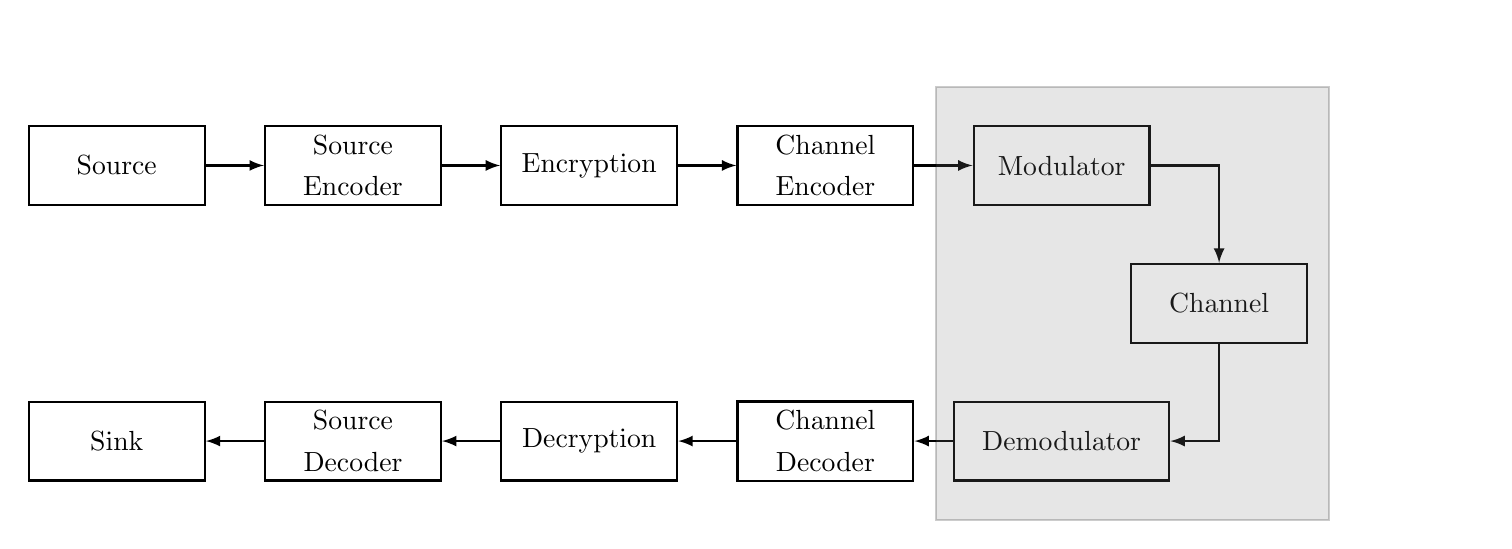
\begin{tikzpicture}[thick]
  \tikzstyle{every node}=[draw,text centered,text width=2cm,minimum height=1cm,shape=rectangle];
    \path (0,0) node (a) {Source}
          (0,1.25) node [draw=none] (aa) {}
          (3,0) node (b) {Source Encoder}
          (3,1.25) node [draw=none] (bb) {}
          (6,0) node (c) {Encryption}
          (6,1.25) node [draw=none] (cc) {}
          (9,0) node (d) {Channel Encoder}
          (9,1.25) node [draw=none] (dd) {}
          (12,0) node (e) {Modulator}
          (14,-1.75) node (f) {Channel}
          (16.25,-1.75) node [draw=none] (ff) {}
          (12,-3.5) node[text width=2.5cm] (g) {Demodulator}
          (9,-3.5) node (h) {Channel Decoder}
          (6,-3.5) node (i) {Decryption}
          (3,-3.5) node (j) {Source Decoder}
          (0,-3.5) node (k) {Sink};

    \draw[-latex] (a) -- (b);
    \draw[-latex] (b) -- (c);
    \draw[-latex] (c) -- (d);
    \draw[-latex] (d) -- (e);
    \draw[-latex] (e) -| (f);
    \draw[-latex] (f) |- (g);
    \draw[-latex] (g) -- (h);
    \draw[-latex] (h) -- (i);
    \draw[-latex] (i) -- (j);
    \draw[-latex] (j) -- (k);

    \filldraw[fill=gray,opacity=0.20] (10.4,1) rectangle (15.4,-4.5);
%    \draw (12.7,-5) node [draw=none,text width=10cm] (gg) {Discrete-Time Equivalent Channel};

\end{tikzpicture}}
\end{center}
\vspace{-4mm}
\caption{The block diagram of a digital communication system where the blocks comprising the discrete-time channel are shaded.}
\end{figure}

In this section, we introduce the \defn{communication}{discrete-time channel model} for digital communication systems.
We will see later that, for some communication systems, this model is exactly equivalent to the more complicated waveform model.
The first channel model we discuss is where the $n$th output of the channel, $Y_n$, is equal to the $n$th input to the channel, $x_n$, corrupted by an additive noise term $Z_n$ so that
\[ Y_n = x_n + Z_n. \]
For this model, it is typical to assume that the noise sequence $Z_1, Z_2, \ldots$ consists of independent identically distributed (i.i.d.) zero-mean Gaussian random variables with variance $\sigma^2$.
This implies that each $Y_n$ is a Gaussian random variable with mean $x_n$ and variance $\sigma^2$, so that
\[ f_{Y_n}(y_n) = \frac{1}{\sqrt{2\pi \sigma^2}} e^{-(y_n - x_n)^2 / (2\sigma^2)}.\]
This model is commonly referred to as discrete-time communication in \defn{communication}{additive white Gaussian noise} (AWGN) noise.

As an example, consider a system where the transmitter sets the voltage on end of a wire and the receiver measures the voltage on the other end of the wire.
It turns out that the thermal agitation of electrons causes voltage fluctuations known as Johnson noise.
So, the receiver ends up measuring the transmitted voltage corrupted by noise fluctuations.
In fact, Johnson noise is quite well approximated by AWGN.
So, the simple model described above already gives a relatively accurate picture of reality.

\section{A Simple Modulation Scheme}

Once a channel model has been defined, the next step is choosing how to transmit digital data through the channel.
A common approach is to choose a small set $\mathcal{U}$ of information symbols and represent each one by a distinct channel input in the set $\mathcal{X}$.
This is the discrete-time model of a scheme known as \defn{communication}{pulse-amplitude modulation} (PAM).
Let $u_n \in \mathcal{U}$ be the information symbol transmitted during the $n$th time interval and $x_n = M(u_n)$ be the $n$th input to the channel, where $M: \mathcal{U} \rightarrow \mathcal{X}$ is called the symbol mapping function.
For example, one can transmit binary information symbols by mapping ``0" to $+1$V and ``1" to $-1$V; mathematically, this is done by choosing $\mathcal{U}=\{0,1\}$, $\mathcal{X}=\{-1,1\}$, and $M(u) = 1-2u$.
This particular type of PAM is called \defn{communication}{binary phase-shift keying} (BPSK) or 2-PAM.

Suppose a BPSK signal is transmitted through our discrete-time AWGN channel model.
The detector must measure the voltage and decide whether a 0 or 1 one was transmitted.
A natural choice is to define a decoder function that associates positive voltages with 0 and negative voltages with 1.
Let $\hat{U}_n = D(Y_n)$ be the output of the detector function
\[ D(y) = \begin{cases} 0 & \text{if }y\geq0 \\ 1 & \text{if }y<0 \end{cases}. \]
This detector is optimal if 0's and 1's are transmitted with equal probability.

One of the main challenges in communication systems is providing reliable data transmission.
In this example, the noise variance $\sigma^2$ is proportional to the power of the thermal noise in the wire.
Notice that, if a 1 is transmitted, the detector described above will make an incorrect decision with probability
\[ \Pr \left( Y_n \geq 0 | x_n = 1 \right) = \Pr \left( Z_n \geq 1 \right) = \int_{1}^{\infty}  \frac{1}{\sqrt{2\pi \sigma^2}} e^{-y^2 / (2\sigma^2)} dy = Q\left( \frac{1}{\sigma} \right).\]
This probability can be reduced by increasing the transmitted voltage, which increases the power dissipated due to resistive losses, or by reducing the thermal noise.
For this reason, receivers used for large satellite dish receivers often use liquid nitrogen to cool the first-stage amplifier to reduce this thermal noise.
On the other hand, the maximum transmitted power is typically limited by physical constraints (e.g., the wire thickness) or FCC regulations.

\begin{figure}[t]
\begin{center}
\scalebox{0.75}
{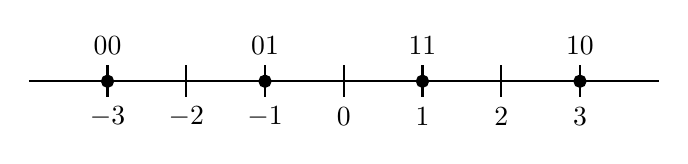
\begin{tikzpicture}[thick]

  \draw (-4,0) -- (4,0);

  \foreach \x in {-3,-2,...,3}
  {
    \draw (\x,-0.20) -- (\x,0.20);
    \draw (\x,-0.45) node {$\x$};
  }

  \foreach \x/\y in {-3/00,-1/01,1/11,3/10}
  {
    \draw (\x,+0.45) node {$\y$};
    \filldraw (\x,0) circle (2pt);
  }

\end{tikzpicture}}
\end{center}
\vspace{-6mm}
\caption{The symbol set $\mathcal{X}$ for 4-PAM with gray coded binary labels.}
\end{figure}

To send more information per channel use, one can use larger sets of PAM symbols.
For example, 4-PAM uses the 4 symbols $\mathcal{X}=\{ -3,-1,1,3 \}$ while 8-PAM uses the 8 symbols $\mathcal{X}=\{-7,-5,-3,-1,1,3,5,7\}$.
Notice that these two sets of symbols are centered around 0 to minimize the transmitted energy.

The mapping function $M(\cdot)$ determines the information symbol associated with each channel input value.
In general, sets of input values with $2^m$ elements are associated with binary strings.
There are still some choices to be made, however, because one can map the 4-PAM symbol set to binary strings in either the standard binary order $\{00,01,10,11\}$ or with a Gray code $\{00,01,11,10\}$.

For the 4-PAM symbol set with the mapping function $M(\cdot)$ that maps $\{00,01,10,11\}$ (in order) to $\{-3,-1,1,3\}$, the natural decision function is
\[ D(y) = \begin{cases}
00 & \text{if }y < -2 \\
01 & \text{if }-2 \leq y<0 \\
10 & \text{if }0 \leq y< 2 \\
11 & \text{if }y \geq 2
\end{cases}. \]

\section{Quadrature Amplitude Modulation}

In most communication systems, the baseband waveform is modulated onto a high-frequency carrier to enable better propagation.
This is because low-frequency signals often do not propagate well through physical media.
While this process will be discussed later in more detail, the following key detail affects the discrete-time model.
High frequency modulation allows two independent signals to be modulated onto the same carrier frequency; one onto the sine wave and the other onto the cosine wave.
This allows one to treat the transmitted value $x_n$ and received value $Y_n$ as points in 2-dimensional space.
The set $\mathcal{X}$ of possible transmitted points in 2-dimensional space in called the \defn{communication}{symbol constellation}.

\begin{figure}
\begin{center}
\scalebox{0.5}
{\begin{tikzpicture}[thick]

  \draw (-4,0) -- (4,0);
  \draw (0,-4) -- (0,4);

  \foreach \x in {-3,-2,...,3}
    \draw (\x,-0.20) -- (\x,0.20);

  \foreach \y in {-3,-2,...,3}
    \draw (-0.20,\y) -- (0.20,\y);

  \foreach \x in {-3,-1,1,3}
  \foreach \y in {-3,-1,1,3}
  {
    \filldraw (\x,\y) circle (2pt);
  }

\end{tikzpicture}}
\hspace{5mm}
\scalebox{0.5}
{\begin{tikzpicture}[thick]

  \draw (-4,0) -- (4,0);
  \draw (0,-4) -- (0,4);

  \foreach \x in {-3,3}
    \draw (\x,-0.20) -- (\x,0.20);

  \foreach \y in {-3,3}
    \draw (-0.20,\y) -- (0.20,\y);

  \foreach \x/\y in {3/0,2.12/2.12,0/3,-2.12/2.12,-3/0,-2.12/-2.12,0/-3,2.12/-2.12}
  {
    \filldraw (\x,\y) circle (2pt);
  }

\end{tikzpicture}}
\end{center}
\caption{The symbol constellations $\mathcal{X}$ for 16-QAM (left) and 8-PSK (right).}
\end{figure}

For mathematical convenience, points in these two-dimensional symbol constellations are represented by complex numbers.
The set of complex numbers is $\mathbb{C}$ and the constellation is a subset $\mathcal{X}\subset\mathbb{C}$.
Likewise, the transmitted symbol is $x_n \in \mathbb{C}$ and the received value is $Y_n \in \mathbb{C}$.
The noise term $Z_n$ now consists of two i.i.d. Gaussian random variables (one in each direction).
The probabilistic observation model is formed by treating the real and imaginary parts separately, and is given by
\begin{align*}
f_{Y^{(r)}_n,Y^{(i)}_n}(y^{(r)}_n,y^{(i)}_n) & =
\left( \frac{1}{\sqrt{2\pi \sigma^2}} e^{-\left(y^{(r)}_n - x^{(r)}_n\right)^2 / (2\sigma^2)} \right)
\left( \frac{1}{\sqrt{2\pi \sigma^2}} e^{-\left(y^{(i)}_n - x^{(i)}_n\right)^2 / (2\sigma^2)} \right) \\
& =  \frac{1}{2\pi \sigma^2} e^{-\left|y_n - x_n\right|^2 / (2\sigma^2)}.
\end{align*}
Therefore, the probability of receiving a $y_n$ value is simply a function of its Euclidean distance $\left| y_n - x_n \right|^2$ from the actual transmitted symbol.
This leads to a nice geometric characterization of the optimal decision regions for the detector.

The \defn{communication}{signal-to-noise ratio} (SNR) of a communication system is typically denoted by $E_s / N_0$ where $E_s$ is the average \textbf{energy per channel input symbol} and $N_0$ is the \defn{communication}{noise spectral density}.
For equiprobable signaling, one finds that
\[ E_s = \frac{1}{|\mathcal{X}|} \sum_{x\in \mathcal{X}} |x|^2. \]
The noise spectral density measures how much the AWGN is affects the channel and later we will see that $N_0 = 2 \sigma^2$ for our discrete-time model.

Constellations are typically defined by first choosing the set of channel input values $\mathcal{X}$, and then choosing the mapping function $M:\mathcal{U} \rightarrow \mathcal{X}$.
This second step is called \textbf{labeling} the constellation.
While the labeling does not affect the symbol error rate of the system, it generally does affect the bit error rate.
Therefore, one can optimize the mapping function for a particular application.

Constellations can be chosen and optimized for a variety of reasons.
Still, there are a few very common choices:
\begin{itemize}
\item $M$-ary PAM ($M$-PAM) is $M$ points equally spaced along a line or
\[ \mathcal{X} = \left\{ 2a-(M-1) \, \big| \, a \in \{0,1,\ldots,M-1\} \right\} \subset \mathbb{C}. \]

\item $M^2$-ary QAM ($M^2$-QAM) is an $M$ by $M$ square grid of points or
\[ \mathcal{X} = \left\{ \left(2a-(M-1)\right)+ \left(2b-(M-1)\right)i \, \big| \, a,b \in \{0,1,\ldots,M-1\} \right\} \subset \mathbb{C}. \]

\item $M$-ary PSK ($M$-PSK) is $M$ points equally spaced around a circle or
\[ \mathcal{X} = \left\{ e^{2\pi i k/M} \, \big| \, k \in \{0,1,\ldots,M-1\} \right\} \subset \mathbb{C}. \]
\end{itemize}

\begin{example}
The standard QAM constellation with 16 points (known as 16-QAM) is given by
\[ \mathcal{X} = \left\{ a+bi \, \big| \, a,b \in \{-3,-1,1,3\} \right\} \subset \mathbb{C}. \]
The average energy of this constellation is given by
\[ E_s = \frac{1}{16} \sum_{a,b\in \{-3,-1,1,3\}} (a^2 + b^2) = \frac{8}{16}  \sum_{a\in \{-3,-1,1,3\}} a^2 = 10.\]
\end{example}

\section{Optimal Symbol Detection}
\index{hypothesis testing}

In this section, we consider the problem of designing a symbol detector that minimizes the probability of error.
This is known as an \defn{communication}{optimal detection} problem and has an elegant solution that is related to the classical problem of \textbf{hypothesis testing} in statistics.

\subsection{Hypothesis Testing}

Sir Ronald Fisher, one of the founders of statistical decision theory, was at a tea party when Ms. Bristol mentioned that she preferred tea poured into milk over milk poured into tea.
Fisher commented that surely she could not tell the difference, but his colleague William Roach suggested that they design an experiment.
At that point, they prepared eight cups of tea: four milk-into-tea and four tea-into-milk.
The cups were presented in a random order and she correctly identified enough (all eight cups by some accounts) to prove her point.

Adding math to this requires that one defines carefully ``can tell the difference", but this is not a big problem because, for example, one can use the hypothesis $H_0=$``her success rate is more than three out of four".
There are more subtle issues, however, such as the meaning of passing the test.
While Ms. Bristol may do this by luck, this is also easy to analyze with calculations.
What is more problematic is understanding all the other hypotheses that can lead to the same observation.
For example, she may pass by cheating but still be unable to distinguish between the two drinks.
If this hypothesis is not explicitly considered, one can come to an incorrect conclusion.

For this reason, any scientific test of a hypothesis can only \emph{disprove} that hypothesis.
If Ms. Bristol cannot get 75\% correct in a larger test, then we can be reasonably confident that ``her ability to distinguish does not meet our threshold of three times out of four".
This is an example of a \defn{hypothesis testing}{null hypothesis} statistical test where the hypothesis can only disproven reliably.
Adding some math to this example shows that
\[ \Pr (\text{she identifies all cups correctly} | H_0 \text{ is false}) \leq (3/4)^8 \approx 0.10. \]
Therefore, the observation does not support the falsification of $H_0$.
Not much more can be concluded from this experiment.

\subsection{Multiple Hypothesis Testing}

Hypothesis testing in communication theory often has the luxury that one of the hypotheses must be true.
This leads to the more well-defined problem of \defn{hypothesis testing}{multiple hypothesis testing}.
Instead of testing a single hypothesis to see if it is false, one can compare multiple hypothesis to see which is most supported by the observation.

Let $H_0,H_1,\ldots,H_{m-1}$ be $m$ different hypotheses that affect a random observation $Y$.
The probability of a hypothesis before the observation, $\Pr(H_i)$, is called the \defn{hypothesis testing}{a priori probability}.
For each hypothesis, the connection with $Y$ is defined by the \defn{hypothesis testing}{observation probability} $\Pr (Y=y \, | \, H_i)$.

The goal is to choose a decision function $D(y)$ which, for any observation, minimizes the decision error probability.
Of course, this is equivalent to maximizing the probability that the decision is correct.
Notice that, if $Y=y$, then the probability that hypothesis $H_i$ is correct is given by its \defn{hypothesis testing}{a posteriori probability} $\Pr (H_i \, | \, Y=y )$.
Therefore, one finds that the optimal choice is the \defn{hypothesis testing}{maximum a posteriori} \textbf{probability} (MAP) decision rule 
\[ D(y) = \underset{i\in\{0,\ldots,m-1\}}{\mathrm{arg\,max}} \Pr( H_i \, |  \, Y=y). \]

In practice, these probabilities can be computed with Bayes' rule using only the a priori probabilities and observation probabilities.
This gives
\[ \Pr \left(H_i | Y=y \right) =
\frac{\Pr(H_i) \Pr (Y=y | H_i) }{\sum_{j=0}^{m-1} \Pr(H_j) \Pr (Y=y | H_j)}. \]
Since the denominator of this expression is the same for all $i$, the MAP rule can be simplified to
\[ D(y) = \underset{i\in\{0,\ldots,m-1\}}{\mathrm{arg\,max}} \Pr(H_i) \Pr (Y=y | H_i). \]

\begin{example}
Consider a system which transmits BPSK over an AWGN channel.
Let $H_0$ be the hypothesis that a zero (i.e., $+1$) was sent and $H_1$ be the hypothesis that a one (i.e., $-1$) was sent.
For binary hypothesis problems, the MAP decision rule can be written as
\[ \Pr (H_0) \Pr (Y=y | H_0) \underset{H_1}{\overset{H_0}{\gtrless}}  \Pr (H_0) \Pr (Y=y | H_0, \]
where this notation implies that one should pick $H_0$ if the LHS is greater than the RHS and $H_1$ otherwise.
If $\Pr(H_0) = 1-p$ and $\Pr (H_1) = p$, then one can substitute formulae to rewrite this as
\[ (1-p)  \frac{1}{\sqrt{2\pi \sigma^2}} e^{-(y-1)^2 / (2\sigma^2)} \underset{H_1}{\overset{H_0}{\gtrless}}  p \frac{1}{\sqrt{2\pi \sigma^2}} e^{-(y+1)^2 / (2\sigma^2)}.\]
After a little algebra, taking the logarithm of both sides simplifies this to 
\[ y \underset{H_1}{\overset{H_0}{\gtrless}} \frac{\sigma^2}{2}  \ln \frac{p}{1-p}.\]
\end{example}

Another popular rule is the \defn{hypothesis testing}{maximum likelihood} (ML) decision rule
\[ D(y) = \underset{i\in\{0,\ldots,m-1\}}{\mathrm{arg\,max}} \Pr (Y=y | H_i), \]
which ignores the a priori probability.
When all the hypotheses have the same a priori probability, these two rules are identical.
In communication systems, this is often the case.

\begin{example}
Consider a system which transmits 4-PAM (i.e, $\mathcal{X}=\{-3,-1,1,3\}$) over an AWGN channel.
If all channel inputs are equiprobable, then the optimum detector is
\begin{align*}
D(y)
& =  \underset{x\in\{-3,-1,1,3\}}{\mathrm{arg\,max}} \left( \frac{1}{\sqrt{2\pi \sigma^2}} e^{-(y-x)^2 / (2\sigma^2)} \right) \\
& =  \underset{x\in\{-3,-1,1,3\}}{\mathrm{arg\,max}} \left(-\frac{1}{2}\ln(2\pi \sigma^2) - \frac{1}{2\sigma^2} (y-x)^2 \right) \\
& =  \underset{x\in\{-3,-1,1,3\}}{\mathrm{arg\,min}} (y-x)^2. 
\end{align*}
Therefore, the optimum detector chooses the constellation point closest to the channel observation.
Moreover, this statement remains true for any signal constellation with equiprobable signalling and AWGN.
\end{example}


\chapter{Fourier Analysis and Sampling}
\label{chapter:FourierAnalysisSampling}

\index{Fourier analysis}
\textbf{Fourier analysis} refers to a collection of tools that can be applied to express a function in terms of complex sinusoids, called basis elements, of different frequencies.
The result of the decomposition is the amplitude and the phase to be imparted to each basis element in the reconstruction.
This decomposition is termed the \defn{Fourier analysis}{frequency domain} representation of the original signal.

Fourier analysis is extremely useful in engineering, with a myriad of applications.
Part of its appeal lies in the fact that basis elements are characteristic functions of linear time-invariant systems.
This property, which may seem nebulous at this point, is instrumental in solving many challenging problems, and makes Fourier analysis a powerful methodology for the design of communication systems.
We assume that the reader is familiar with basic Fourier analysis, and only review details that are pertinent to our treatment of communication systems.
This is not intended to be a comprehensive treatment of the subject.


\section{Fourier Series}
\label{section:FourierSeries}

Fourier series can be employed to express, as weighted sums of sinusoidal components, either periodic functions or functions that are time-limited.
Suppose that $s(t)$ is a function that is nonzero only for $-\frac{T}{2} \leq t \leq \frac{T}{2}$, and is square integrable
\begin{equation*}
\| s(t) \|^2 \triangleq \int_{\mathbb{R}} |s(t)|^2 dt
= \int_{-\frac{T}{2}}^{\frac{T}{2}} |s(t)|^2 dt < \infty .
\end{equation*}
Then $s(t)$ possesses a \defn{Fourier analysis}{Fourier series} representation, which is defined by
\begin{equation} \label{equation:FourierSeries1}
s(t) = \begin{cases} \sum_{k=-\infty}^{\infty}
\hat{s}_k e^{2 \pi i \frac{k}{T} t}, & |t| \leq \frac{T}{2} \\
0, & \text{otherwise} \end{cases}
\end{equation}
where the Fourier series coefficients $\{ \hat{s}_k : k \in \mathbb{Z} \}$ are given by
\begin{equation*}
\hat{s}_k = \frac{1}{T} \int_{-\frac{T}{2}}^{\frac{T}{2}}
s(t) e^{-2 \pi i \frac{k}{T} t} dt .
\end{equation*}
We can use the standard rectangular function $\mathrm{rect}(\cdot)$, defined by
\begin{equation} \label{equation:RectangularFunction}
\mathrm{rect} (t) = \begin{cases} 1, & |t| < 0.5 \\
0, & \text{otherwise} \end{cases}
\end{equation}
to simplify \eqref{equation:FourierSeries1}, and rewrite the Fourier representation of $s(t)$ as
\begin{equation} \label{equation:FourierSeries2}
s(t) = \sum_{k=-\infty}^{\infty}
\hat{s}_k e^{2 \pi i \frac{k}{T} t}
\mathrm{rect} \left( \frac{t}{T} \right) .
\end{equation}
From a vector space perspective, \eqref{equation:FourierSeries2} asserts that $s(t)$ can be expressed as a linear combination of basis elements $\{ \theta_k (t) : k \in \mathbb{Z} \}$, where
\begin{equation*}
\theta_k (t) = e^{2 \pi i \frac{k}{T} t} \mathrm{rect} \left(\frac{t}{T} \right) .
\end{equation*}
Furthermore, note that the collection of functions $\{ \theta_k (t) : k \in \mathbb{Z} \}$ forms an orthogonal set under the standard inner product; that is,
\begin{equation*}
\begin{split}
\left\langle \theta_k(t), \theta_n(t) \right\rangle
&= \int_{-\infty}^{\infty} \theta_k(t) \theta_n^*(t) dt
= \int_{-\frac{T}{2}}^{\frac{T}{2}} e^{2 \pi i \frac{k}{T} t}
e^{- 2 \pi i \frac{n}{T} t} dt \\
&= \int_{-\frac{T}{2}}^{\frac{T}{2}} e^{2 \pi i \frac{(k-n)}{T} t} dt
= 0
\end{split}
\end{equation*}
for all $k \neq n$.
An interesting and important aspect of Fourier series is that time-limited functions can be characterized using a discrete set of coefficients.
This fact provides insight into the sampling theorem, which we will review shortly.


\section{Fourier Transforms}

The \defn{Fourier analysis}{Fourier transform} applies to functions that are not necessarily time-limited.
Assume that $x(t)$ is a signal that is square integrable,
\begin{equation} \label{equation:L2Condition}
\| x(t) \|^2 = \int_{\mathbb{R}} | x(t) |^2 dt < \infty .
\end{equation}
Then, we can express $x(t)$ using its frequency domain representation.
The Fourier transform of $x(t)$, which we denote by $\hat{x}(f)$ or $\mathcal{F} [x(t)]$, is defined by
\begin{equation} \label{equation:FourierTransform}
\hat{x}(f) = \mathcal{F} [x(t)]
= \int_{\mathbb{R}} x(t) e^{-2 \pi i f t} dt .
\end{equation}
The original function can subsequently be expressed in terms of its decomposition,
\begin{equation} \label{equation:InverseFourierTransform}
x(t) = \int_{\mathbb{R}} \hat{x}(f) e^{2 \pi i f t} df .
\end{equation}
We sometimes denote the inverse Fourier transform of $\hat{x}(f)$ as $\mathcal{F}^{-1} [\hat{x}(f)]$.
It is interesting to point out the duality between the Fourier transform and its inverse, $\mathcal{F} \left[ \hat{x} (t) \right] = x(-f)$.
This relation is rooted in the striking similarity between \eqref{equation:FourierTransform} and \eqref{equation:InverseFourierTransform}.

\begin{example}[Rectangular Pulse]
The rectangular pulse $\mathrm{rect} (\cdot)$, defined in \eqref{equation:RectangularFunction}, can be used to constrain various signals in time or frequency.
Note that $\| \mathrm{rect} (t) \|^2 = 1 < \infty$, which guarantees that Fourier analysis can be applied to this function.
The Fourier transform of $\mathrm{rect} (t)$ can be computed as follows,
\begin{equation*}
\begin{split}
\mathcal{F} \left[ \mathrm{rect} (t) \right]
&= \int_{\mathbb{R}} \mathrm{rect} (t) e^{- 2 \pi i f t} dt
= \int_{-\frac{1}{2}}^{\frac{1}{2}} e^{- 2 \pi i f t} dt \\
&= \frac{1}{\pi f} \left( \frac{e^{\pi i f} - e^{- \pi i f}}{2i} \right)
= \frac{ \sin \pi f }{\pi f} \\
&= \mathrm{sinc}(f) .
\end{split}
\end{equation*}
Thus, the Fourier transform of $\mathrm{rect}(\cdot)$ is the famous $\mathrm{sinc}(\cdot)$ function, which plays a fundamental role in the sampling and reconstruction of information signals.
\end{example}

The Fourier transform $\hat{x}(f)$ of a square-integrable signal $x(t)$ also allows one to pose the question, ``How much signal energy is contained the frequencies between $f_0$ and $f_1$?".
The answer, for $f_0 \leq f_1$, is given by the integral
\[ \int_{f_0}^{f_1} \left| \hat{x}(f) \right|^2 df. \]
This integral exposes the quantity $\mathcal{G}_x (f) = \left| \hat{x}(f) \right|^2$ as the \defn{Fourier analysis}{energy spectral density} of $x(t)$.
For technical reasons, we actually define the energy spectral density later in terms of its Fourier transform.
In practice, the answer to the above question also depends on whether the signal is real or complex.
For real signals, the integral is typically computed over the range $f_0 < |f| < f_1$.

When condition~\eqref{equation:L2Condition} is not satisfied, it may be hazardous to use Fourier analysis and frequency domain representations.
Strictly speaking, the Fourier transform of a function may not exist if it behaves wildly.
Casually taking the Fourier transforms of arbitrary signals should be avoided.
Having said that, there will be instances where we discuss the Fourier transforms of functions that do not fulfill \eqref{equation:L2Condition};
one such example appears below.
We adopt this somewhat cavalier attitude because experience allows us to avoid pitfalls, and Fourier relaxation leads to great engineering insight.
The downside of this approach is that the reader is left with the burden of deciding whether a signal has a proper spectral representation, or if the definition of the Fourier transform is being applied loosely.

Starting with signal $x(t)$, we can write
\begin{equation} \label{equation:NestedFourierRepresentation}
\begin{split}
x(t) &= \int_{\mathbb{R}} \hat{x}(f) e^{2 \pi i f t} df
= \int_{\mathbb{R}} \left[ \int_{\mathbb{R}} x(\tau) e^{-2 \pi i f \tau} d\tau \right] e^{2 \pi i f t} df \\
&= \int_{\mathbb{R}} \left[ \int_{\mathbb{R}} e^{2 \pi i f (t - \tau)} df \right] x(\tau) d\tau ,
\end{split}
\end{equation}
where the second equality follows from \eqref{equation:FourierTransform} and the third equality is obtained by changing the order of integration.
Recall that we can use the Dirac delta function $\delta(t)$ to write (informally)
\begin{equation*}
x(t) = \int_{\mathbb{R}} \delta (t - \tau) x(\tau) d\tau .
\end{equation*}
Since \eqref{equation:NestedFourierRepresentation} holds for any time~$t$, we find that
\begin{equation*}
\delta (t) = \int_{\mathbb{R}} e^{2 \pi i f t} df 
\end{equation*}
is one representation of $\delta(t)$ and hence the (cavalier) Fourier transform of the $\delta$-function is $\mathcal{F} [ \delta(t) ] = 1$.


\subsection{Periodic Signals}
\label{section:PeriodicSignals}

We can develop (cavalier) Fourier transform representations for periodic signals as well, thereby providing a unified treatment of periodic and aperiodic functions. 
Indeed, we can construct the Fourier transform of a periodic signal directly from its Fourier series representation.
Let $x(t)$ be a signal with Fourier transform $\hat{x}(f) = \delta (f - f_0)$.
To recover the signal $x(t)$, we can apply the inverse Fourier transform
\begin{equation*}
x(t) = \mathcal{F}^{-1} [ \delta (f - f_0) ]
=\int_{\mathbb{R}} \delta (f - f_0) e^{2 \pi i f t} df
= e^{2 \pi i f_0 t}.
\end{equation*}
More generally, if $\hat{x}(f)$ is a linear combination of impulses equally spaced in frequency
\begin{equation} \label{equation:PeriodicFrequency}
\hat{x}(f) = \sum_{k = -\infty}^{\infty} \hat{s}_k \delta (f - k f_0) ,
\end{equation}
then its inverse Fourier transform becomes
\begin{equation} \label{equation:PeriodicTime}
x(t) = \sum_{k = -\infty}^{\infty} \hat{s}_k e^{2 \pi i k f_0 t} .
\end{equation}
Note that \eqref{equation:PeriodicTime} corresponds to the Fourier series representation of a periodic signal.
Thus, the Fourier transform of a periodic signal with Fourier series coefficients $\{ \hat{s}_k : k \in \mathbb{Z} \}$ can be interpreted as a train of impulses in the frequency domain.

A signal that will be useful in our analysis of sampling is the impulse train
\begin{equation*}
x(t) = \sum_{k = -\infty}^{\infty} \delta(t - kT) .
\end{equation*}
This is a special case of a periodic function, with period $T$.
We can therefore apply a methodology similar to the one derived above to compute its Fourier transform.
The Fourier series coefficients for the impulse train are obtained as
\begin{equation*}
\hat{s}_k = \frac{1}{T} \int_{-\frac{T}{2}}^{\frac{T}{2}}
x(t) e^{- 2 \pi i \frac{k}{T} t} dt
= \frac{1}{T} .
\end{equation*}
Using \eqref{equation:PeriodicFrequency}, we get
\begin{equation} \label{equation:ImpulseTrainFrequency}
\hat{x}(f)
= \frac{1}{T} \sum_{k = -\infty}^{\infty} \delta \left( f - \frac{k}{T} \right) .
\end{equation}
Surprisingly, an impulse train in the time domain can be regarded as an impulse train in the frequency domain.
A second representation for $x(t)$ is given by \eqref{equation:PeriodicTime},
\begin{equation} \label{equation:ImpulseTrainTime}
x(t) = \sum_{k = -\infty}^{\infty} \delta(t - kT)
= \frac{1}{T} \sum_{k = -\infty}^{\infty} e^{2 \pi i \frac{k}{T} t} .
\end{equation}
Which representation to use depends on the problem at hand.


\subsection{Spectral Density}
\label{subsection:SpectralDensity}

The energy content of a deterministic signal $x(t)$ is given by \eqref{equation:L2Condition}.
If the energy content of $x(t)$ is finite, i.e.\ $\| x(t) \|^2 < \infty$, then we can define its \defn{Fourier analysis}{autocorrelation function} by
\begin{equation*}
R_x(\tau) = \int_{\mathbb{R}} x(t)x^*(t - \tau) dt .
\end{equation*}
Using this notation, we can write the energy content of $x(t)$ as $R_x(0)$.

\begin{definition}
The \defn{Fourier analysis}{energy spectral density} of $x(t)$, denoted by $\mathcal{G}_x (f)$, is defined to be the Fourier transform of its autocorrelation function,
\begin{equation*}
\mathcal{G}_x(f) = \mathcal{F} [ R_x (\tau) ] = | \hat{x}(f) |^2.
\end{equation*}
\end{definition}

Intuitively, the energy spectral density captures the frequency content of a signal and helps identify how its energy is distributed across frequencies.
The \defn{Fourier analysis}{spectral bandwidth} of Fourier transform $\hat{x}(f)$ is the smallest value of $W$ such that $\mathcal{G}_x(f) = 0$ for all $|f| > W$.
A signal $x(t)$ is \defn{Fourier analysis}{bandwidth-limited} to $W$ if it can be obtained as the inverse Fourier transform of a function $\hat{x}(f)$, where $\hat{x}(f)$ is identically zero for all $|f| > W$.


\subsection{Linear Time-Invariant Filters}
\label{subsection:LinearTimeInvariantFilters}

The importance of the Fourier transform comes, partly, from its ability to capture the effects of linear time-invariant filters on deterministic signals.
Suppose that the input to a linear time-invariant filter is $x(t)$, then its output is given by
\begin{equation*}
y(t) = x(t) \ast h(t),
\end{equation*}
where $h(t)$ is the impulse response of the linear filter and $\ast$ denotes the convolution operator.
If we use $\hat{h}(f)$ to represent the Fourier transform of impulse response $h(t)$, then the output signal in the frequency domain becomes
\begin{equation*}
\hat{y}(f) = \hat{x}(f) \hat{h}(f) .
\end{equation*}
That is, convolution in the time domain becomes multiplication in the frequency domain, a much simpler operation.
The output signal can then be recovered by taking the inverse Fourier transform of $\hat{y}(f)$,
\begin{equation*}
y(t) = \mathcal{F}^{-1} [ \hat{y}(f) ] = \mathcal{F}^{-1} [ \hat{x}(f) \hat{h}(f) ] .
\end{equation*}
This also implies that the spectral density, $\mathcal{G}_y(f)$, of $y(t)$ satisfies
\[ \mathcal{G}_y(f) = \mathcal{G}_x(f) \mathcal{G}_h(f). \]

\section{Sampling Deterministic Signals}

The sampling theorem is one of the most significant results in communications.
Many digital communication systems rely on the validity of this theorem and on the design insights it provides for proper operation.
The basic idea behind the sampling theorem can be summarized in a few words.
If a signal $x(t)$ is bandwidth-limited to $W$, then this signal can be reconstructed from a collection of samples so long as the samples are taken at periodic intervals of $T \leq \frac{1}{2W}$.
A formal version of the sampling theorem appears below.

\begin{theorem}[Sampling Theorem] \label{theorem:SamplingTheorem}
Let signal $x(t)$ be a bandwidth-limited function with bandwidth $W$.
If $x(t)$ is sampled at times $\{ nT : n \in \mathbb{Z} \}$ where $T \leq \frac{1}{2W}$, then it is possible to reconstruct the original signal $x(t)$ from its sampled points $\{ x(nT) : n \in \mathbb{Z} \}$.
Specifically, if $T \leq \frac{1}{2W}$ then
\begin{equation} \label{equation:SamplingReconstructionFormula}
x(t) = \sum_{n = -\infty}^{\infty}
x(nT) \mathrm{sinc} \left( \frac{t}{T}-n \right) .
\end{equation}
\end{theorem}
\begin{proof}
The signal $x(t)$ is bandwidth-limited with bandwidth $W$.
It follows that $x(t)$ is the inverse Fourier transform of a function $\hat{x}(f)$, where $\hat{x}(f) = 0$ for all frequencies such that $|f| > W$.
For convenience, we define $F = \frac{1}{T}$ and we stress that $W \leq \frac{1}{2T} = \frac{F}{2}$.
Thus, $\hat{x}(f) = 0$ whenever $|f| > \frac{F}{2}$.
We can apply the theory of Fourier series introduced in Section~\ref{section:FourierSeries} to express $\hat{x}(f)$ as
\begin{equation*}
\hat{x}(f) = \sum_{k=-\infty}^{\infty} s_k e^{2 \pi i \frac{k}{F} f}
\mathrm{rect} \left( \frac{f}{F} \right)
\end{equation*}
where the coefficients $\{ s_k : k \in \mathbb{Z} \}$ are equal to
\begin{equation*}
s_k
= \frac{1}{F} \int_{-\frac{F}{2}}^{\frac{F}{2}}
\hat{x}(f) e^{- 2 \pi i \frac{k}{F} f} df .
\end{equation*}
Special care should be taken when reading these equations because we are applying Fourier series analysis to a function in the frequency domain.
This can get confusing.

We can then write $x(t)$ in terms of basis elements,
\begin{equation*}
\begin{split}
x(t) &= \mathcal{F}^{-1} \left[ \hat{x}(f) \right]
= \mathcal{F}^{-1} \left[ \sum_{k=-\infty}^{\infty} s_k e^{2 \pi i \frac{k}{F} f}
\mathrm{rect} \left( \frac{f}{F} \right) \right] \\
&= \sum_{k=-\infty}^{\infty} s_k \mathcal{F}^{-1} \left[ e^{2 \pi i \frac{k}{F} f}
\mathrm{rect} \left( \frac{f}{F} \right) \right] \\
%&= \sum_{k=-\infty}^{\infty} s_k
%\int_{-\frac{F}{2}}^{\frac{F}{2}} e^{2 \pi i \frac{k}{F} f} e^{2 \pi i f t} df \\
%&= \sum_{k=-\infty}^{\infty} s_k
%\int_{-\frac{F}{2}}^{\frac{F}{2}} e^{2 \pi i \left( t + \frac{k}{F} \right) f} df \\
%&= \sum_{k=-\infty}^{\infty} s_k
%\frac{e^{\pi i \left( t + \frac{k}{F} \right) F} - e^{-\pi i \left( t + \frac{k}{F} \right) F}}{2 \pi i \left( t + \frac{k}{F} \right)} \\
%&= \sum_{k=-\infty}^{\infty} s_k
%\frac{\sin \left( \pi \left( t + \frac{k}{F} \right) F \right)}{\pi \left( t + \frac{k}{F} \right)} \\
%&= \sum_{k=-\infty}^{\infty} s_k F \mathrm{sinc} \left( F t + k \right) \\
&= \sum_{k=-\infty}^{\infty} \frac{s_k}{T} \mathrm{sinc} \left( \frac{t}{T} + k \right) .
\end{split}
\end{equation*}
Above, we have successively used the scaling and time-shift properties of the Fourier transform.
We can obtain the values of $\{ s_k : k \in \mathbb{Z} \}$ explicitly by exploiting the characteristics of the $\mathrm{sinc} (\cdot)$ function,
\begin{equation*}
x(nT)
= \sum_{k=-\infty}^{\infty}
\frac{s_k}{T} \mathrm{sinc} \left( \frac{nT}{T} + k \right)
= \sum_{k=-\infty}^{\infty}
\frac{s_k}{T} \mathrm{sinc} ( n + k ) = \frac{s_{-n}}{T} .
\end{equation*}
Thus, we have $s_{k} = T x(-kT)$ and formula \eqref{equation:SamplingReconstructionFormula} follows.
The sampling rate corresponding to $T = \frac{1}{2W}$ is the minimum rate at which perfect reconstruction is possible.
It is called the \defn{Fourier analysis}{Nyquist rate}.
\end{proof}

We can gain better intuition about sampling using the Fourier transform representation for periodic signals developed in Section~\ref{section:PeriodicSignals}.
Let $x_{\mathrm{s}}(t)$ denote the result of sampling $x(t)$ by impulses at times $\{ nT : n \in \mathbb{Z} \}$,
\begin{equation*}
x_{\mathrm{s}}(t) = x(t) \sum_{n=-\infty}^{\infty} \delta(t-nT)
= \sum_{n=-\infty}^{\infty} x(nT) \delta(t-nT).
\end{equation*}
Looking at the sampled signal in the frequency domain, we get
\begin{equation*}\begin{split}
\hat{x}_{\mathrm{s}}(f) &= \hat{x}(f) \ast \mathcal{F} \left[ \sum_{n=-\infty}^{\infty} \delta(t-nT) \right] \\
&= \hat{x}(f) \ast \frac{1}{T} \sum_{n=-\infty}^{\infty} \delta \left( f-\frac{n}{T} \right) \\
&= \frac{1}{T} \sum_{n=-\infty}^{\infty} \hat{x} \left( f - \frac{n}{T} \right) ,\end{split}\end{equation*}
where we have used \eqref{equation:ImpulseTrainFrequency} to express the Fourier transform of an impulse train.
When the sampling rate is fast enough, the translated copies of $\hat{x}(f)$ contained in the transform $\hat{x}_{\mathrm{s}}(f)$ do not overlap, and the original signal can be recovered using an ideal lowpass filter.
However, when the sampling period~$T$ is too small, the various copies of $\hat{x}(f)$ overlap and the content of the original is partially destroyed.
This is know as \defn{Fourier analysis}{aliasing}.

\begin{figure}[htbp]
\begin{center}
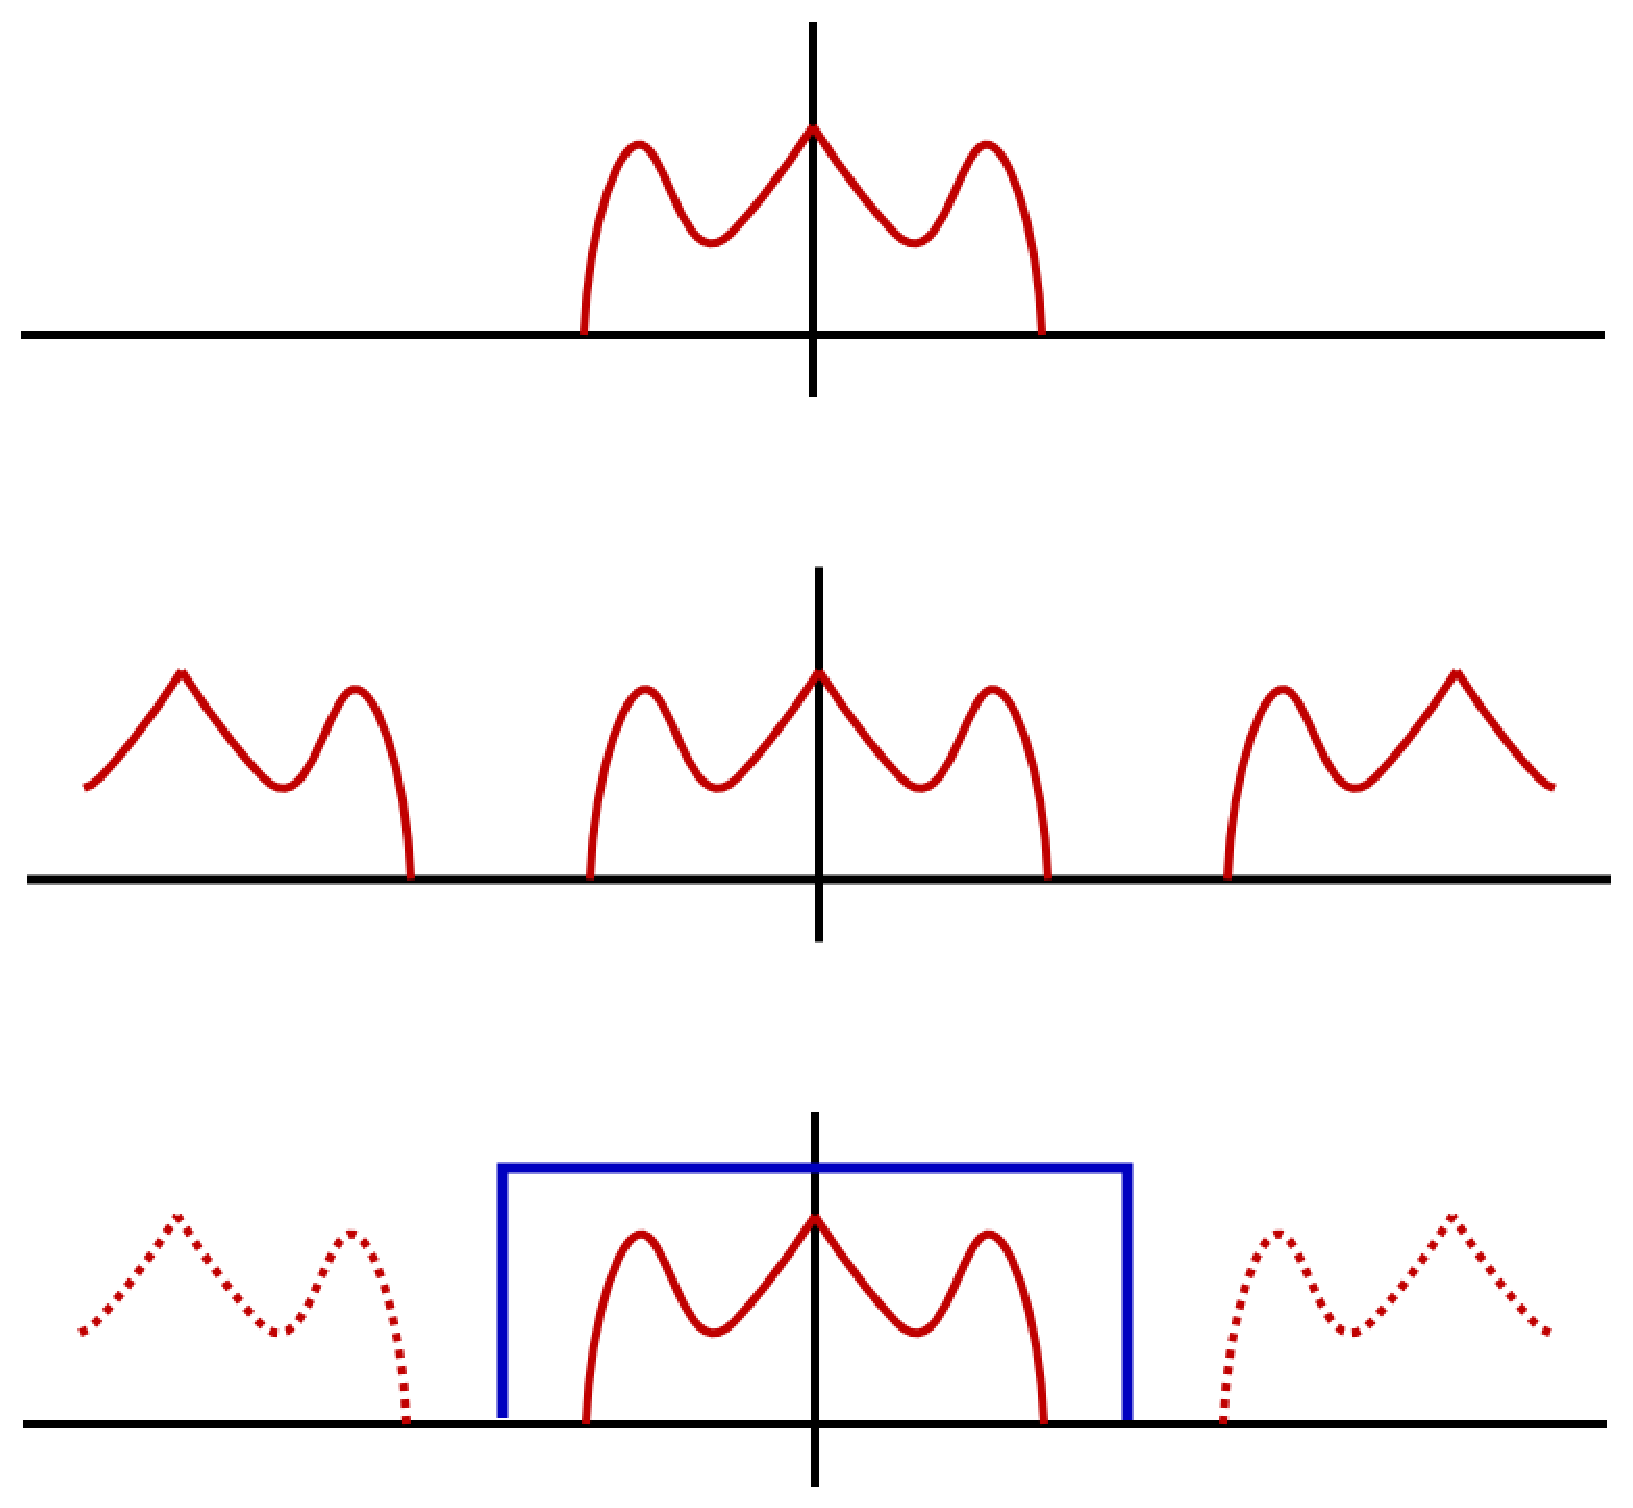
\epsfig{file=Figures/sampling,width=8cm}
\caption{The sampling and reconstruction of a bandwidth-limited signal.
When the sampling rate exceeds twice the bandwidth of the original signal, this signal can be reconstituted from its sampled values.}
\label{figure:Sampling}
\end{center}
\end{figure}
A succession of power spectral densities can be found on Figure~\ref{figure:Sampling}.
The top component shows the power spectral density of the original signal.
The density of the sampled signal appears below.
Finally, the reconstruction operation where a lowpass filter is employed to recovered the original function is illustrated at the bottom of the figure.
In contrast, Figure~\ref{figure:Aliasing} exhibits a case where the sampling frequency is too low.
\begin{figure}[htbp]
\begin{center}
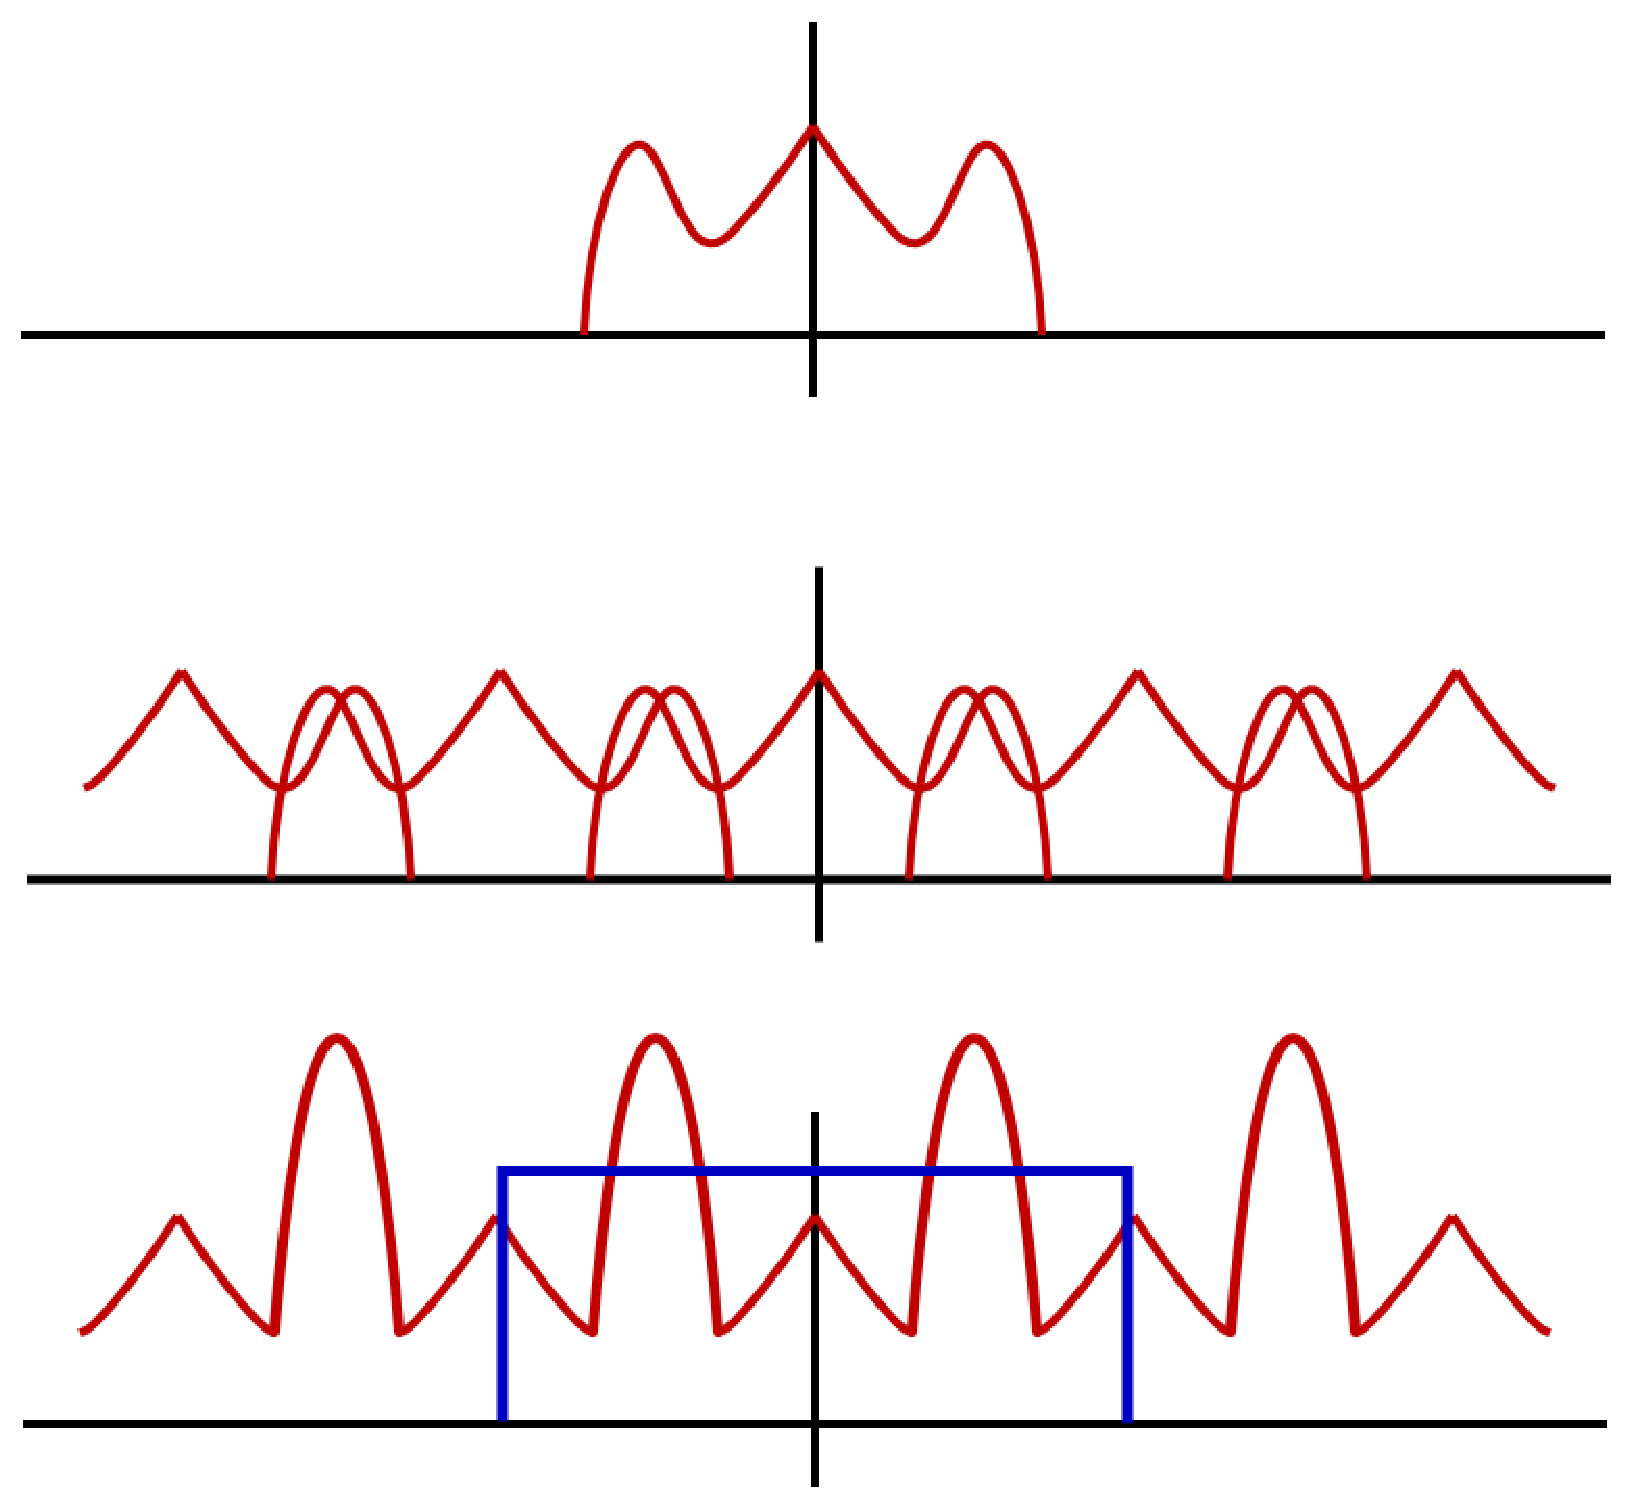
\epsfig{file=Figures/aliasing,width=8cm}
\caption{A low sampling frequency leads to aliasing, thereby preventing reconstruction of the original signal.}
\label{figure:Aliasing}
\end{center}
\end{figure}
Aliasing in the frequency domain prevents the original signal from being retrieved.

The illusion of a moving image in video is achieved by displaying a rapid succession of still pictures over time.
Films are typically shot at a rate of twenty-four frames per second, whereas the minimum frame rate required to create the appearance of a moving image is about fifteen frames per second.
The human eye acts as a lowpass filter and transforms the succession of images into a live video.
High-speed cameras are used to record slow-motion playback movies.
As a consequence, they must run at much higher frame-rates than normal cameras.

\subsection{Imperfect Sampling and Reconstruction}

In practice, it is impossible to measure (i.e., sample) a signal $x(t)$ instantaneously.
A more realistic model is that the sample value is given by the integral
\[ \int_{\mathbb{R}} x(t) p(t-nT) dt, \]
for some sampling waveform $p(t)$.
In this case, the resulting samples are identical to the perfect sampling of the filtered waveform $y(t)=x(t)*p(-t)$.
Therefore, the sample values are given by
\[ y(nT) = \int_{\mathbb{R}} x(t) p(t-nT) dt. \]
It also follows that, if no aliasing occurs, the imperfection can be eliminated completely using a discrete-time filter to equalize the resulting samples.

A similar imperfection occurs during reconstruction.
In practice, it is not possible to weight each sample by the exact sinc interpolation waveform.
Instead, the samples $x(nT)$ are weighted by some arbitrary pulse shape $p(t)$.
In this case, the reconstruction output is given by
\[ y(t) = \sum_{n=-\infty}^{\infty} x(nT) p(t-nT). \]
Since $p(t-nT) = \delta(t-nT) * p(t)$, we can see this instead as perfect reconstruction followed by filtering and write
\[ y(t) = \left( \sum_{n=-\infty}^{\infty} x(nT) \delta (t-nT) \right) * p(t) = x(t) * p(t). \]
Again, it follows that this imperfection can therefore be eliminated completely by post-filtering.
The main advantage in practice is that one can jointly optimize both $p(t)$ and the post-filter to provide good performance while using inexpensive components.


\section{Stochastic Signals}
\label{section:StocahsticSignalsFAS}
\index{random process}

A \textbf{random process} (or \defn{random process}{stochastic process}) is an extension of the concept of random variable to the situation where the values of a signal are not known beforehand.
Mathematically, a stochastic process can be viewed in two different ways.
First, the process can be thought of as an instantiation of a random experiment where the outcome is selected from a collection of time functions.
Alternatively, a stochastic process can be viewed as a collection of random variables indexed by time.
If the index set corresponds to the real numbers, then the process is a \defn{random process}{continuous-time} \textbf{random process}.
Whereas if the index set is discrete, then it is a \defn{random process}{discrete-time} \textbf{random process}.
The viewpoint where a stochastic process is regarded as a collection of random variables tends to prevail in the study of digital communications.
\begin{figure}[htbp]
\begin{center}
\begin{psfrags}
\psfrag{A}[c]{Amplitude}
\psfrag{t}[c]{Time}
\psfrag{t0}[c]{$t_0$}
\psfrag{t1}[c]{$t_1$}
\epsfig{file=Figures/process,width=7cm}
\end{psfrags}
\caption{Two distinct abstractions of a random process.
It can be viewed as the output of an experiment where a function is selected at random.
Alternatively, a random process may be taken as a set of random variables indexed by time.}
\label{figure:RandomProcess}
\end{center}
\end{figure}

Random processes are frequently employed in the design of communication systems.
For example, they can be used to model the data originating from a source, channel variations, noise and interference.
Their importance will become evident as we progress through these notes.
In general, it is difficult to provide a complete mathematical description for a random process.
For now, we restrict our attention to \defn{random process}{stationary} and \defn{random process}{ergodic} random processes.

\begin{definition}[Stationarity]
A random process $X(t)$ is wide-sense stationary if its \defn{random process}{mean}
\begin{equation*}
m_X(t) = \mathrm{E} [X(t)]
\end{equation*}
is independent of time, and its \defn{random process}{autocorrelation function}, defined by
\begin{equation*}
R_X(t_1, t_2) = \mathrm{E} [X(t_1) X^*(t_2)],
\end{equation*}
only depends on the difference between $t_1$ and $t_2$.
With a slight abuse of notation, we can denote the mean and autocorrelation of a stationary process respectively by $m_X$ and $R_X(\tau)$, where $\tau = t_1 - t_2$.
\end{definition}

\begin{definition}[Ergodicity]
The \defn{random process}{ergodic theorems} assert that, under certain conditions, the time average of a function along all the possible trajectories of a random process exists and is equal to its ensemble average,
\begin{equation*}
\lim_{T \rightarrow \infty} \frac{1}{T} \int_{- \frac{T}{2}}^{\frac{T}{2}} g(X(t)) dt
= \mathrm{E}[g(X(t))] .
\end{equation*}
When a stochastic process fulfills these conditions, it is called \defn{random process}{ergodic}.
\end{definition}

\begin{figure}[htbp]
\begin{center}
\begin{psfrags}
\psfrag{A}[c]{Amplitude}
\psfrag{t}[c]{Time}
\psfrag{t0}[c]{$t_0$}
\psfrag{m}[c]{$m_X$}
\psfrag{e}[c]{$\lim_{T \rightarrow \infty} \frac{1}{T} \int_{- \frac{T}{2}}^{\frac{T}{2}} X(t) dt$}
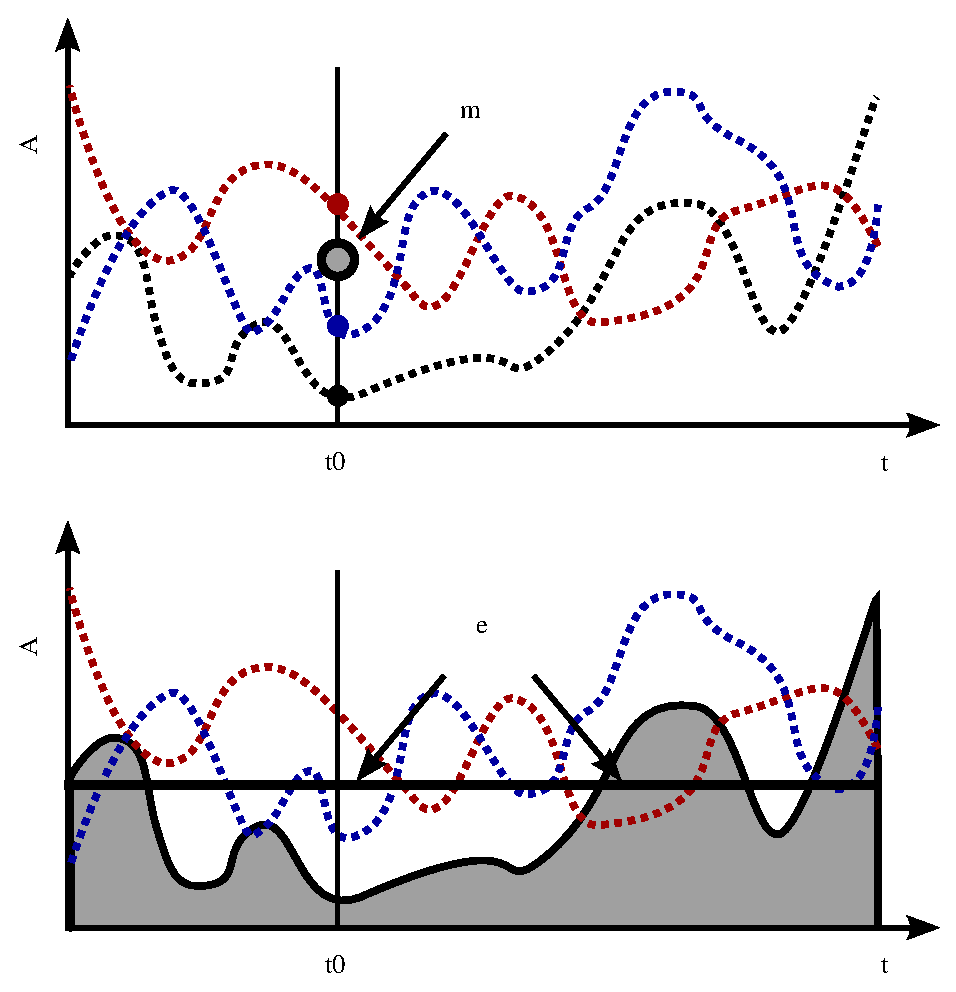
\epsfig{file=Figures/ergodic,width=8cm}
\end{psfrags}
\caption{For ergodic processes, the time average of a function along a trajectory is equal to the ensemble average.}
\label{figure:ErgodicProcess}
\end{center}
\end{figure}

One of the important characteristics of an ergodic process is that it suffices to look at one realization of the process to infer many of its statistical attributes.
Ergodicity is a very strong property, and it is hard to test and validate.
Rather, it is frequently taken as a premise in the design of communication systems.
For instance, most information sources are assumed to be stationary and ergodic.
Such a postulate appears reasonable, especially given the many successful communication systems implemented to date.


\subsection{Power Spectral Density}

The \defn{random process}{power spectral density} of a stochastic signal is an extension to the spectral density discussed in Section~\ref{subsection:SpectralDensity}.
The definition of the power spectral density is somewhat more intricate due to the more complex nature of random signals.
In particular, it must account for uncertainty in the process.

Let $X(t)$ be a wide-sense stationary and ergodic random process, with $R_X(0) < \infty$.
The Fourier transform of a specific realization of $x(t)$ may not exist, as it need not fulfill condition \eqref{equation:L2Condition}.
However, a truncated version of $x(t)$ possesses a Fourier transform.
Consider the truncated version of $x(t)$ given by
\begin{equation*}
x_T(t) = x(t) \mathrm{rect} \left( \frac{t}{T} \right) ,
\end{equation*}
and its Fourier transform
\begin{equation*}
\hat{x}_T(f) = \mathcal{F} \left[ x(t) \mathrm{rect} \left( \frac{t}{T} \right) \right] .
\end{equation*}
The power spectral density of $X(t)$ represents the amount of power per hertz of bandwidth present in the signal at various frequencies, and it is defined by
\begin{equation*}
\mathcal{S}_X(f) = \lim_{T \rightarrow \infty} \frac{1}{T} \mathrm{E} \left[ |\hat{x}_T(f)|^2 \right] .
\end{equation*}
Note how the truncated signal is used to overcome the difficulty of dealing with infinite-energy signals.
This is a common and valuable trick.
As we will soon see, the power spectral density plays an instrumental role in the sampling theorem for random signals.
First, we provide a means to compute $\mathcal{S}_X(f)$ from its statistical attributes.

\begin{theorem}[Wiener-Khinchin]
The power spectral density $\mathcal{S}_X (f)$ of a wide-sense stationary random process $X(t)$ is equal to the Fourier transform of its autocorrelation function, $\mathcal{S}_X (f) = \mathcal{F} [R_X (\tau)]$.
\end{theorem}
\begin{proof}
For a wide-sense stationary process, we have
\begin{equation*}
\begin{split}
\mathcal{S}_X(f) &= \lim_{T \rightarrow \infty} \frac{1}{T} \mathrm{E} \left[ |\hat{x}_T(f)|^2 \right]
= \lim_{T \rightarrow \infty} \frac{1}{T} \mathrm{E} \left[ \hat{x}_T(f) \hat{x}_T^*(f) \right] \\
&= \lim_{T \rightarrow \infty} \frac{1}{T} \mathrm{E} \left[
\int_{-\frac{T}{2}}^{\frac{T}{2}} X(t_1) e^{-2 \pi i f t_1} dt_1
\int_{-\frac{T}{2}}^{\frac{T}{2}} X^*(t_2) e^{2 \pi i f t_2} dt_2 \right] \\
&= \lim_{T \rightarrow \infty} \frac{1}{T}
\int_{-\frac{T}{2}}^{\frac{T}{2}} \int_{-\frac{T}{2}}^{\frac{T}{2}}
\mathrm{E} \left[ X(t_1) X^*(t_2) \right]
e^{-2 \pi i f (t_1-t_2)} dt_1 dt_2 \\
&= \int_{\mathbb{R}} R_X (\tau) e^{-2 \pi i f\tau} d\tau
= \mathcal{F} [ R_X (\tau) ] .
\end{split}
\end{equation*}
The fourth equality is obtained by interchanging the expectation and the integrals, while the sixth equality follows from a change of variables and the fact that $X(t)$ is wide-sense stationary.
To guarantee that the former operation is legitimate, $\tau R_X(\tau)$ must remain finite for all $\tau$.
\end{proof}


\subsection{Filtering Stochastic Processes}

We discussed in Section~\ref{subsection:LinearTimeInvariantFilters} how the Fourier transform can simplify the analysis of the effects of linear time-invariant filters on deterministic signals.
In this section, we consider the operation of such filters in the context of random processes.

\begin{theorem}
If a wide-sense stationary process $X(t)$ with mean $m_X$ and autocorrelation function $R_X(\tau)$ is passed through a linear time-invariant filter with impulse response $h(t)$, then the output process $Y(t)$ has mean
\begin{equation*}
m_Y = m_X \int_{\mathbb{R}} h(t) dt
\end{equation*}
and its autocorrelation is equal to
\begin{equation*}
R_Y (\tau) = R_X(\tau) \ast h(\tau) \ast h^*(-\tau) .
\end{equation*}
\end{theorem}
\begin{proof}
The output process at time~$t$ is given by $Y(t) = \int_{\mathbb{R}} X(t - \xi) h(\xi) d\xi$.
We can therefore obtain the expectation of $Y(t)$ as follows,
\begin{equation*}
\begin{split}
m_Y (t) &= \mathrm{E} \left[ \int_{\mathbb{R}} X(t - \xi) h(\xi) d\xi \right]
= \int_{\mathbb{R}} \mathrm{E} \left[ X(t - \xi) \right] h(\xi) d\xi \\
&= m_X \int_{\mathbb{R}} h(\xi) d\xi.
\end{split}
\end{equation*}
We emphasize that $m_Y$ is independent of time.

To derive the autocorrelation function for $Y(t)$, we first compute the cross-correlation between $X(t)$ and $Y(t)$,
\begin{equation} \label{equation:CrossCorrelationLTI}
\begin{split}
\mathrm{E} [X(t_1) Y^*(t_2) ]
&= \mathrm{E} \left[ X(t_1) \int_{\mathbb{R}} X^*(\xi) h^*(t_2 - \xi) d\xi \right] \\
&= \int_{\mathbb{R}} \mathrm{E} \left[ X(t_1) X^*(\xi) \right] h^*(t_2 - \xi) d\xi \\
&= \int_{\mathbb{R}} R_X(t_1 - \xi) h^*(t_2 - \xi) d\xi \\
%&= \int_{\mathbb{R}} R_X(\tau - \xi) h^*(- \xi) d\xi \\
&= R_X(\tau) \ast h^*(-\tau) .
\end{split}
\end{equation}
This shows that the cross-correlation between $X(t)$ and $Y(t)$ depends only on $\tau$; we can therefore express it as $R_{XY}(\tau)$.
We are now ready to compute the autocorrelation function for $Y(t)$.
\begin{equation} \label{equation:AutoCorrelationLTI}
\begin{split}
\mathrm{E} [Y(t_1) Y^*(t_2) ]
&= \mathrm{E} \left[ \int_{\mathbb{R}} X(\xi) h(t_1 - \xi) d\xi Y^*(t_2) \right] \\
&= \int_{\mathbb{R}} \mathrm{E} \left[ X(\xi) Y^*(t_2) \right] h(t_1 - \xi) d\xi \\
&= \int_{\mathbb{R}} R_{XY}(\xi - t_2) h(t_1 - \xi) d\xi \\
%&= \int_{\mathbb{R}} R_{XY}(\xi) h(\tau - \xi) d\xi \\
&= R_{XY}(\tau) \ast h(\tau) .
\end{split}
\end{equation}
Substituting $R_{XY} (\tau)$ by the equivalent expression $R_X(\tau) \ast h^*(-\tau)$ from \eqref{equation:CrossCorrelationLTI}, we get the desired result.
We observe that the autocorrelation of the process $Y(t)$ only depends on the difference between $t_1$ and $t_2$, and hence $Y(t)$ is also wide-sense stationary.
\end{proof}

Obtaining an expression for the autocorrelation function corresponding to the output of a linear time-invariant filter allows us to characterize the power spectral density of the output process.
In terms of the frequency representation, we get $m_Y = m_X \hat{h}(0)$ and
\begin{equation*}
\begin{split}
\mathcal{S}_Y (f) &= \mathcal{F} [ R_Y (\tau) ] \\
&= \mathcal{F} \left[ R_X (\tau) \ast h(\tau) \ast h^*(-\tau) \right] \\
&= \mathcal{S}_X(f) | \hat{h}(f) |^2 .
\end{split}
\end{equation*}
A linear time-invariant filter can be employed to shape the spectrum of a stochastic process, and to constrain its bandwidth.
This is an important result, as linear filters can be used to reduce the bandwidth of a random signal before sampling or to reconstruct a random signal from its samples.


\section{Sampling Bandlimited Processes}

We know from Theorem~\ref{theorem:SamplingTheorem} that a bandwidth-limited signal can be perfectly reconstructed from its samples provided that the sampling rate exceeds twice the bandwidth of the original signal.
At this point, one may wonder whether it is possible to extend the sampling theorem to bandwidth-limited stochastic processes.
This question is answered in the affirmative below.

\begin{theorem} \label{theorem:SamplingRandomSignals}
Suppose that $X(t)$ is a wide-sense stationary bandwidth-limited process with bandwidth $W$ and power spectral density $\mathcal{S}_X (f)$.
Let $\tilde{X}(t)$ be an approximation for $X(t)$ built from the sampled values $\{ X(nT) : n \in \mathbb{Z} \}$,
\begin{equation*}
\tilde{X}(t) = \sum_{n=-\infty}^{\infty} X(nT) \mathrm{sinc} (2 W (t - nT)) ,
\end{equation*}
where $T = \frac{1}{2W}$ denotes the sampling interval.
Then the mean-squared error between the original random process and the reconstructed version vanishes,
\begin{equation} \label{equation:SamplingMSE}
\left\| X(t) - \tilde{X}(t) \right\|^2
= \mathrm{E} \left[ \left| X(t) - \sum_{n=-\infty}^{\infty}
X(nT) \mathrm{sinc} (2 W (t - nT)) \right|^2 \right] = 0 .
\end{equation}
The expectation in \eqref{equation:SamplingMSE} is over all possible realizations of $X(t)$.
\end{theorem}
\begin{proof}
To establish this result, we expand the mean-squared error of \eqref{equation:SamplingMSE},
\begin{equation*}
\begin{split}
&\left\| X(t) - \tilde{X}(t) \right\|^2
= \mathrm{E} \left[ \left| X(t) - \sum_{n=-\infty}^{\infty} X(nT)
\mathrm{sinc}(2 W (t - nT)) \right|^2 \right] \\
&= R_X(0) - \sum_{n=-\infty}^{\infty} [ R_X(t-nT) + R_X^*(t-nT) ]
\mathrm{sinc}(2 W (t - nT)) \\
&+ \sum_{n=-\infty}^{\infty} \sum_{m=-\infty}^{\infty} R_X((m-n)T)
\mathrm{sinc}(2 W (t - mT)) \mathrm{sinc}(2 W (t - nT)) .
\end{split}
\end{equation*}
The double summation above can be rewritten as
\begin{equation*}
\begin{split}
&\sum_{n=-\infty}^{\infty} \sum_{k=-\infty}^{\infty} R_X(kT)
\mathrm{sinc}(2 W (t - kT - nT)) \mathrm{sinc}(2 W (t - nT)) \\
&\sum_{n=-\infty}^{\infty} \left( \sum_{k=-\infty}^{\infty} R_X(kT)
\mathrm{sinc}(2 W (t - kT - nT)) \right) \mathrm{sinc}(2 W (t - nT)) \\
&= \sum_{n=-\infty}^{\infty} R_X(t - nT) \mathrm{sinc}(2 W (t - nT)) ,
\end{split}
\end{equation*}
where the last equality follows from the sampling theorem for deterministic signals (Theorem~\ref{theorem:SamplingTheorem}).
Putting these results together, we get
\begin{equation*}
\left\| X(t) - \tilde{X}(t) \right\|^2
= R_X(0) - \sum_{n=-\infty}^{\infty} R_X^*(t-nT) \mathrm{sinc}(2 W (t - nT)) .
\end{equation*}
Applying Theorem~\ref{theorem:SamplingTheorem} one more time and noticing that $R_X(0) = R_X^*(0)$, we obtain $\| X(t) - \tilde{X}(t) \|^2 = 0$, as desired.
\end{proof}

Theorem~\ref{theorem:SamplingRandomSignals} is important because it confirms that the design insights gained from analyzing deterministic signals hold for random signals as well.


\section{Bandpass Signals and Processes}

One possible application of sampling is to take a continuous-time signal and to transform it into a discrete-time signal.
For instance, this operation gives the information coming out of a source a format more suitable for digital communications.
This prime application of sampling served as the original motivation for our study of the subject.
A second possible application of sampling is the processing of received waveforms at the output of communication channels.
In digital communications, the data often assumes the form of an analog carrier signal modulated by a digital bit stream.
Mathematically, this situation is captured by the equation
\begin{equation*}
y(t) = x(t) \cos (2 \pi f_{\mathrm{c}} t) .
\end{equation*}
The signal $y(t)$ is a special form of a \defn{Fourier analysis}{bandpass signal}.
Its Fourier transform $\hat{y}(f)$ is non-zero only for frequencies contained in a small neighborhood of carrier frequency $f_{\mathrm{c}}$.
That is, $\hat{y}(f) = 0$ for all frequencies such that $|f - f_{\mathrm{c}}| \geq W$.
To apply the sampling tools derived above to the information bearing signal $x(t)$, we need to shift the corresponding spectrum to the origin.

The Fourier transform of $y(t)$ is given by
\begin{equation*}
\hat{y}(f) = \frac{1}{2} \hat{x}(f+f_{\mathrm{c}}) + \frac{1}{2} \hat{x}(f - f_{\mathrm{c}}) .
\end{equation*}
Our strategy is to first eliminate $\frac{1}{2} \hat{x}(f + f_{\mathrm{c}})$ from $\hat{y}(f)$, and then to scale and shift $\frac{1}{2} \hat{x}(f + f_{\mathrm{c}})$ back to the origin.
Define the \defn{Fourier analysis}{step function} by
\begin{equation*}
\mathrm{step} (t) = \frac{1}{2} + \frac{1}{2} \mathrm{sign}(t). 
\end{equation*}
Taking the (cavalier) Fourier transform of $\mathrm{step}(t)$, we get
\begin{equation*}
\begin{split}
{\mathcal{F}} [\mathrm{step} (t)]
&= {\mathcal{F}} \left[ \frac{1}{2} + \frac{1}{2} \mathrm{sign}(t) \right] \\
&= \frac{1}{2} \delta (f)
- \frac{1}{2} \int_{-\infty}^0 e^{-2 \pi i ft} dt
+ \frac{1}{2} \int_0^{\infty} e^{-2 \pi i ft} dt \\
&= \frac{1}{2} \delta(f)  + \frac{1}{2 \pi i f}.
\end{split}
\end{equation*}
Using the duality property of the Fourier transform, we get
\begin{equation*}
\mathcal{F}^{-1} [\mathrm{step}(f)] = \frac{1}{2} \delta(t) + \frac{i}{2 \pi t} .
\end{equation*}
And, by construction, we obtain $\hat{x}(f - f_{\mathrm{c}}) = 2 \mathrm{step}(f) \hat{y}(f)$.
We can therefore recover the original lowpass signal $x(t)$ using the frequency-shift property of the Fourier transform,
\begin{equation*}
x(t)
= \left[ y(t) \ast \left( \delta (t) + \frac{i}{\pi t} \right) \right]
e^{- 2 \pi i f_{\mathrm{c}} t}
= \left[ y(t) + i \left( y(t) \ast \frac{1}{\pi t} \right) \right] e^{- 2 \pi i f_{\mathrm{c}} t} .
\end{equation*}
The second component of this signal,
\begin{equation*}
y(t) \ast \frac{1}{\pi t} ,
\end{equation*}
is called the \defn{Fourier analysis}{Hilbert transform} of $y(t)$.
Once $x(t)$ is brought back to baseband, the standard sampling theorem applies and a discrete-time version of the signal can be produced.

% Bandpass processes

\chapter{Quantization}

\index{quantization}
As mentioned in the introduction, two operations are necessary to transform an analog waveform into a digital signal.
The first action, sampling, consists of converting a continuous-time input into a discrete-time function.
The second operation is the process of approximating continuous-space sample values by a discrete set of possible points.
This process, termed \textbf{quantization}, is also essential to transmit an analog signal over digital media.
Quantization invariably induces a loss in signal quality.
The \defn{quantization}{distortion} between the original and quantized functions is usually unwanted, and cannot be reversed.
Yet, for a specific application, the level of signal degradation can be controlled.

In this chapter, we focus primarily on the quantization of real numbers.
The techniques described here can easily be extended to complex numbers by quantizing the real and imaginary parts separately.
In a more abstract sense, the quantization of a complex number is equivalent to vector quantization for a pair of real numbers.


\section{Scalar Quantizers}

Quantizers can generally be designed to be very robust for a large class of signals.
In scalar quantization, each source value is processed individually; the input value is mapped to an output taking one of finitely many values.
The number of quantization levels is typically chosen to be a power-of-2 because the outputs are usually represented using binary strings.
Mathematically, a quantizer is a function taking value in a finite set.
The input to the quantizer is a real number and the output belongs to set $\mathcal{Q}$.
Then, one can define the quantizer as a function $Q : \mathbb{R} \mapsto \mathcal{Q}$ with output
\begin{equation*}
x_{\mathrm{q}} = Q(x) .
\end{equation*}
This is perhaps best seen through an example.


\begin{example}
Let $Q : \mathbb{R} \mapsto \mathcal{Q}$ be a quantizer with four possible outputs labeled $q_1$ through $q_4$.
The output $x_{\mathrm{q}}$ of the quantizer belongs to set $\mathcal{Q}$, and it must therefore be equal to one of the four possible points listed above.
Figure~\ref{figure:Quantizer} shows the functional representation of a four-level quantization scheme.
\begin{figure}[htbp]
\begin{center}
\begin{psfrags}
\psfrag{q1}[l]{$q_1$}
\psfrag{q2}[l]{$q_2$}
\psfrag{q3}[l]{$q_3$}
\psfrag{q4}[l]{$q_4$}
\psfrag{o}[c]{Output}
\psfrag{i}[c]{Input}
\epsfig{file=Figures/quantizer,width=6cm}
\end{psfrags}
\caption{This is a functional representation of a quantizer where the input is converted to one of four possible values.}
\label{figure:Quantizer}
\end{center}
\end{figure}
The output of the quantizer in this example is determined according to a nearest neighbor rule and this implies that
\[ Q(x) =
\begin{cases}
q_1 & \mathrm{if }\; x < \frac{q_1 + q_2}{2} \\
q_2 & \mathrm{if }\; \frac{q_1 + q_2}{2} \leq x < \frac{q_2 + q_3}{2} \\
q_3 & \mathrm{if }\; \frac{q_2 + q_3}{2} \leq x < \frac{q_3 + q_4}{2} \\
q_4 & \mathrm{if }\; x \geq \frac{q_3 + q_4}{2} 
\end{cases}. \]
We note that this quantization function is not one-to-one and, therefore, does not have an inverse.
\end{example}


\section{Distortion Measures}

To compare different quantizers, a performance metric must be established.
A common distortion measure with desirable properties is the square of the error
\begin{equation} \label{equation:QuantizationErrorSquared}
d(x, x_{\mathrm{q}}) = \left|x - Q(x) \right|^2 ,
\end{equation}
where $x - x_{\mathrm{q}}$ is called the \defn{quantization}{quantization error}.
The expression in \eqref{equation:QuantizationErrorSquared} measures how close the output $x_{\mathrm{q}}$ is to the input for a specific value of $x$.
It is popular in communications and signal processing because it is proportional to the increase in noise power caused by quantization.

When a quantizer is employed to discretize the value of a sampled waveform, it is appropriate to evaluate the performance of the quantizer in terms of the difference between the original function and the reconstructed version rather than the distortion between the sample values themselves.
Suppose that $x(t)$ is a bandwidth-limited process with bandwidth $W$.
We know that this process can be accurately recovered from the sampled values $\{ x(nT) : n \in \mathbb{Z} \}$ using the formula
\begin{equation*}
x(t) = \sum_{n = -\infty}^{\infty} x(nT) \mathrm{sinc} \left( \frac{t}{T} - n \right)
\end{equation*}
where $T \leq \frac{1}{2W}$.
Assume that the sampled values are quantized before reconstruction, with
\begin{equation*}
x_{\mathrm{q}} (nT) = Q ( x(nT) ) .
\end{equation*}
A legitimate question is, how close is the approximation $x_{\mathrm{q}}(t)$ to the original signal $x(t)$ using the quantized data
\begin{equation*}
x_{\mathrm{q}}(t) = \sum_{n = -\infty}^{\infty} x_{\mathrm{q}}(nT) \mathrm{sinc} \left( \frac{t}{T} - n \right) ,
\end{equation*}
is anywhere close to $x(t)$.
A useful performance criterion is the energy in the qunatization error signal,
\begin{equation*}
\int_{\mathbb{R}} \left| x(t) - x_{\mathrm{q}} (t) \right|^2 dt ,
\end{equation*}
which quantifies the total distortion between the original and reconstructed signals.
Using Parseval's identity, we get
\begin{equation*}
\begin{split}
&\int_{\mathbb{R}} \left|  x(t) - x_{\mathrm{q}} (t) \right|^2 dt
= \int_{\mathbb{R}} \left| \hat{x} (f) - \hat{x}_{\mathrm{q}} (f) \right|^2 df \\
&= \int_{\mathbb{R}} \left| \sum_{n = -\infty}^{\infty}
\frac{\left( x(nT) - x_{\mathrm{q}}(nT) \right)}{2W} e^{2 \pi i \frac{n}{2 W} f}
\mathrm{rect} \left( \frac{f}{2W} \right) \right|^2 df \\
&= \sum_{n = -\infty}^{\infty}
| x(nT) - x_{\mathrm{q}}(nT) |^2 .
\end{split}
\end{equation*}
Above, we have used the fact that the basis elements
\begin{equation*}
\left\{ e^{2 \pi i \frac{n}{2 W} f} \mathrm{rect} \left( \frac{f}{2W} \right) : n \in \mathbb{Z} \right\}
\end{equation*}
are orthogonal.
Minimizing the quantization error for individual samples turns out to also minimize the overall squared error between the original and reconstructed waveforms $x(t)$ and $x_{\mathrm{q}}(t)$.


\subsection{Mean Squared Error}

Since the quantizer is designed to operate on an information signal, a more relevant assessment of performance weighs in the accuracy of the quantizer over all possible realizations of the random input.
An appropriate distortion measure for the quantization of a stochastic signal is provided by the \defn{quantization}{mean squared error} (MSE),
\begin{equation} \label{equation:QuantizationMSE}
\mathrm{E} [ d(X, X_{\mathrm{q}}) ]
= \mathrm{E} \left[ \left( X - Q(X) \right)^2 \right] .
\end{equation}
Note that this performance metric depends on the distribution of the input signal, and hence is tied to a specific application.
A quantizer can be said to work well in a particular context.
However, describing the performance of a quantization scheme without specifying the distribution of its input signal is meaningless.

\begin{example} \label{example:UniformQuantizer}
Suppose that the values of a discrete-time information signal are uniformly distributed over $[0,16]$.
Furthermore, assume that the quantizer implements a nearest neighbor rule with quantization levels equal to $q_m = 2m - 1$ for $m = 1, 2, \ldots, 8$.
We wish to find the mean squared error of this quantization scheme.

Being uniformly distributed, the probability density function of the input is
\begin{equation*}
f_X (x) = \frac{1}{16}
\end{equation*}
for $x \in [0, 16]$, and zero otherwise.
The decision regions corresponding to the various quantization points are given by $[0, 2], (2, 4], \ldots, (14, 16]$.
We can therefore compute the mean squared error as follows,
\begin{equation*}
\begin{split}
\mathrm{E} [ d(X, X_{\mathrm{q}}) ]
&= \mathrm{E} \left[ \left( X - Q(X) \right)^2 \right]
= \int_0^{16} \frac{(x - Q(x))^2}{16} dx \\
&= \sum_{m=1}^8 \int_{2m-2}^{2m} \frac{(x - (2m - 1))^2}{16} dx \\
&= \frac{1}{2} \int_{0}^{2} (x - 1)^2 dx = \frac{1}{3} .
\end{split}
\end{equation*}
That is, the mean squared error associated with this input distribution and quantization scheme is $\mathrm{E} \left[ (X - Q(X))^2 \right] = \frac{1}{3}$.
\end{example}



\subsection{Signal to Quantization-Noise Ratio}

One of the criticisms about the MSE of \eqref{equation:QuantizationMSE} is that it has a tendency to assign a larger distortion value to signal input with larger second moments.
Indeed, an information process likely to feature large amplitudes is bound to yield outputs with a large mean squared error.
On the other hand, under this absolute metric, most quantizers may appear to work well for minute signals as their mean squared errors are destined to remain small.
A normalized version of this criterion that takes into consideration the power of the original signal is the \defn{quantization}{signal-to-quantization-noise ratio} (SQNR),
\begin{equation} \label{equation:SQNR}
\text{SQNR}
= \frac{\mathrm{E} \left[ X^2 \right]}{\mathrm{E} \left[ (X - Q(X))^2 \right]} .
\end{equation}
Because of the implicit normalization associated with \eqref{equation:SQNR}, this latter measure is more suitable to compare quantizer performance for different input processes.
Like many quantities in communications and signal processing, the value is often specified in decibels by applying the function $10\log_{10}(\cdot)$.

\begin{example}
Assume that the values of a discrete-time information signal are uniformly distributed over $[0,2]$.
We denote the input signal in the present problem using $Y$.
We wish to obtain the mean squared error associated with the quantizer of Example~\ref{example:UniformQuantizer}, applied to the signal at hand.
Also, we wish to compare the SQNR of the quantization scheme of Example~\ref{example:UniformQuantizer} with the SQNR of the scenario described in this example.

To derive the mean squared error, we follow the same steps as before
\begin{equation*}
\begin{split}
\mathrm{E} [ d(Y, Y_{\mathrm{q}}) ]
&= \int_0^{2} \frac{(y - Q(y))^2}{2} dy \\
&= \frac{1}{2} \int_{0}^{2} (y - 1)^2 dy = \frac{1}{3} .
\end{split}
\end{equation*}
We notice that the MSE is the same as the one derived in Example~\ref{example:UniformQuantizer}.
Nevertheless, the quantization scheme seems more suited to the signal described in the previous example.
The SQNR of the current scheme is given by
\begin{equation*}
\text{SQNR} = \frac{\mathrm{E}[Y^2]}{\mathrm{E} [ d(Y, Y_{\mathrm{q}}) ]}
= 3 \mathrm{E}[Y^2] = 4 \approx 6.02 \, \text{dB}.
\end{equation*}
This can be compared with the SQNR of the problem featured in Example~\ref{example:UniformQuantizer}, which is given by
\begin{equation} \label{equation:UniformQuantizerSQNR}
\text{SQNR} = \frac{\mathrm{E}[X^2]}{\mathrm{E} [ d(X, X_{\mathrm{q}}) ]}
= 3 \mathrm{E}[X^2] = 256 \approx 24.08 \, \text{dB}.
\end{equation}
Obviously, the SQNR is much better in the case of Example~\ref{example:UniformQuantizer}.
Can you think of an eight-level quantization scheme that would perform better for the current problem, perhaps rivaling the SQNR of \eqref{equation:UniformQuantizerSQNR}?
\end{example}

Both the mean squared error and the signal-to-quantization-noise ratio are valid and meaningful ways to present performance results for quantization schemes.
Still, they must be put in proper context, especially when comparing scenarios where the distributions of the input signals differ.
For a fixed input process, a quantization scheme that minimizes the MSE will invariably maximize the SQNR.

\begin{example}[Quantization Rule of Thumb]
Consider a signal whose amplitude is bounded between -1 and 1 and whose amplitude distribution has a uniform distribution over the same range.
Suppose that $n$ bits are represent $2^n$ uniformly spaced quantization levels $q_m = -1-2^{-n} + m 2^{-n+1}$ for $m=1,\ldots,2^n$.
The performance as a function of $n$ is typically approximated by the rule that the \textbf{SQNR increases by 6.02 dB per bit} for additional quantization bits.

In this case, the quantizer function is
\[ Q(x) =
\begin{cases}
-1+2^{-n} & \mathrm{if} \; x < -1 \\
\frac{1}{2^{n-1}} \left( \lfloor 2^{n-1} x \rfloor - \frac{1}{2} \right) & \mathrm{if} \; - 1 \leq x < 1 \\
1+2^{-n} & \mathrm{if} \; x \geq 1.
\end{cases}
\]
By symmetry, the distribution of the quantization error is the same for each quantization cell so it suffices to calcluate
\begin{align*}
\mathrm{E} \left[ \left( X - Q(X) \right)^2 \big| Q(X)=2^{-n} \right]
&= \int_{0}^{2^{-n+1}} f_{X|Q(X)=2^{-n}}(x) (x-2^{-n})^2 dx \\
&= \int_{0}^{2^{-n+1}} 2^{n-1} (x^2-2^{-n+1}x+2^{-2n}) dx \\
&= \frac{2^{-2n+2}}{3} - \frac{2^{-2n+2}}{2} + 2^{-2n} \\
&= \frac{2^{-2n}}{3}.
\end{align*}
Since $E[X^2] = 2/3$, the SQNR in decibels is therefore given by
\[ \text{SQNR} = 10 \log_{10} \left( \frac{2\cdot 3}{3\cdot 2^{-2n}} \right)  = (2n+1) 10 \log_{10} 2 \approx 6.02 n + 3.01 \, \text{dB}. \]
As we expected, the SQNR increases by 6.02 dB per bit.
What is surprising is that, for large $n$,  this rule holds for any continuous amplitude distribution supported on $[-1,1]$.
\end{example}

\subsection{Dithering}

While the SQNR accurately measures the increase in noise power caused by quantization, it does not give any information about the spectral content of the quantization noise.
For many applications it is also important that the quantization noise is white (i.e., uncorrelated in time).
To see the problem with standard quantization, consider the periodic signal $x_n$ that satisfies $x_{n+N} = x_n$.
In this case, the quantized version $y_n = Q(x_n)$ and the quantization error $e_n = y_n - x_n$ are also periodic.
Therefore, the spectral energy of the quantization noise is concentrated in the harmonics of the fundamental frequency.

Since the quantizer affects only value at a time, one might wonder how the quantization noise becomes correlated.
The mechanism for this is that the quantization noise is correlated with input value.
For example, one can compute this correlation for the quantizer in Example~\ref{example:UniformQuantizer} and see that
\begin{align*}
\mathrm{E} \left[X \left(X - Q(X)\right) \right] 
&= \int_0^{16} \frac{x(x - Q(x))}{16} dx \\
&= \sum_{m=1}^8 \int_{2m-2}^{2m} \frac{x(x - (2m - 1))}{16} dx \\
&= \sum_{m=1}^8 \int_{2m-2}^{2m} \frac{x(x - (2m - 1))}{16} dx \\
&= \frac{1}{2} \int_{0}^{2} (x+(2m-2))(x - 1) dx \\
&= \frac{1}{2} \int_{0}^{2} x(x - 1) dx = \frac{1}{3}.
\end{align*}
From this, we see that the correlation is the same as the MSE.
This means that quantizing a pure sinusoid will typically create new spurious harmonics whose powers are proportional to the power in the original sinusoid.

The process of adding a small amount of noise before quantization is called \defn{quantization}{dithering}.
Of course, the added noise increases the overall noise power in the system by a small amount.
But, if then noise is chosen to be i.i.d. uniform over one quantization interval, then correlation becomes exactly zero.
Now, we let $Z$ be a uniform random variable on $[-1,1]$ and notice that
\[  \mathrm{E} \left[Q(X+Z)|X=x \right] = \int_{-1}^{1} \frac{1}{2} Q(x+z) dz = x. \]
From this, we can repeat the calculation from above to see that
\begin{align*}
\mathrm{E} \left[X \left(X - Q(X+Z)\right) \right] 
&= \int_0^{16} \int_{-1}^{1} \frac{x(x - Q(x+z))}{32} dz \, dx \\
&= \int_0^{16} \frac{x(x - x)}{16} dz \, dx \\
&= 0.
\end{align*}
This implies that the quantization noise is uncorrelated with the signal.
One can also show that it is white (i.e., uncorrelated with time-shifts of itself).


\subsection{Non-Uniform Quantization Via Companding}

Uniform quantizers are quite robust because their performance is relatively insensitive to the input distribution.
When the input statistics are not uniform, it is possible to design a non-uniform quantizer with the same number of levels and lower SQNR.
One way of doing this is by quantizing the signal after it is processed by a \textbf{compressor}.
After reconstruction, an \textbf{expander} is used to reverse the effect of the compresor.
Since quantization occurs after compression, the quanitization levels are effectively remapped by the compressor.
This whole process is called \defn{quantization}{companding}.

Let the compressor $g(x)$ be an invertible function mapping real numbers to real numbers.
Then, one has $X_q = g^{-1} \left( Q \left( g(X) \right) \right)$.
When the quantization step size $\Delta$ is small, the step size $\Delta'$ after compression can be approximated by
\[ \Delta' = \frac{\Delta}{g'(x)}. \]
This allow one to approximate the quantization noise variance by
\[ E \left[ (X_q - X)^2 \right] = \frac{\Delta^2}{12} \int_{-x_0}^{x_0} \frac{f_X (x)}{|g'(x)|^2} dx, \]
where the quantization levels cover the range $[-x_0,x_0]$.
Under the same assumption, the optimum compressor is proportional to
\[ g(x) = \int_{0}^{x} \sqrt[3]{f_X (z)} dz . \]

For signals with a wide dynamic range, the SQNR depends heavily of the local average signal power.
Using a logarithmic compressor allows one efficiently quantize these signal so that the SQNR is independent of local signal power.
Since larger quantization cells are used for large signal values, the quantization noise naturally scales with the signal power.
For audio signals, the perceptual effect of noise typically depends more on the SQNR than the noise power.
Therefore, logarithmic compression is natrual choice for such signals.

In fact, transforms of this type have been standardized for use in the telephone system.
The standard transform in the United States is called $\mu$-law companding and maps uniformly spaced 14-bit samples into non-uniformly spaced 8-bit samples.
The resulting distortion is not easily undetectable by the human ear.
The $\mu$-law companding algorithm maps $[-1,1]$ to $[-1,1]$ using the rule, for some $\mu >0$,
\[ g(x) = \mathrm{sgn}(x)\frac{\ln \left( 1+ \mu |x| \right)}{\ln (1+\mu)}. \]

The benefits of companding are actually due to two different mechanisms.
First, the amplitude distribution of speech decays rapidly, so it makes sense to include more quantization levels in the small signal range.
Adjusting for this correctly actually increases the SQNR.
Second, human perception of audio depends on the SQNR instead of the noise power.
So, matching the quantization noise to the perceptual measure improves perceived quality.
In many cases, however, it is possible that the SQNR decreases while the perceived quality increases.


\section{Optimal Quantization}

\subsection{Uniform Quantizers}
\label{section:UniformQuantizers}

Finding an optimal quantizer is not an easy task.
An eight-level quantizer has eight degrees of freedom, and the overall performance of the quantizer is jointly determined by the positions of the quantization points.
A means to reduce the difficulty of identifying an optimal quantization scheme is to constrain the possible candidates.
This can be achieved, for instance, by imposing a rule on the respective position of the quantization points.
Restricting the search space to uniform quantizers is one possible way to ensure that an optimal quantizer can be found.

A \defn{quantization}{uniform quantizer} is a function where the locations of successive outputs are situated at a fixed interval, $q_m - q_{m-1} = \Delta$ for all the possible values.
That is, the distance between two quantization points is the same for all neighbors.
This scheme is one of the simplest quantizer designs.
The quantization function considered in Figure~\ref{figure:Quantizer} is in fact a uniform quantizer.
If the objective function of the optimization process is the mean squared error, then optimal locations for the quantization points can be found in a straightforward manner.
First, note that we can write the position of the quantization points as
\begin{equation*}
q_m = q_1 + (m-1) \Delta
\end{equation*}
for $m = 1, 2, \ldots, M$ where $M$ is the number quantization levels.
As usual, the MSE is given by
\begin{equation*}
\mathrm{E} [ d(X, X_{\mathrm{q}}) ]
= \int_{\mathbb{R}} (x - Q(x))^2 f_X(x) dx .
\end{equation*}
We emphasize  that the performance of the quantizer is optimized by minimizing the value of the integrand at each point.
We deduce that the decision regions corresponding to $q_1, q_2, \ldots, q_M$ must be equal to
\begin{equation*}
\left( - \infty, q_1 + \frac{\Delta}{2} \right],
\left( q_2 - \frac{\Delta}{2}, q_2 + \frac{\Delta}{2} \right],
\ldots,
\left( q_M - \frac{\Delta}{2}, \infty \right) ,
\end{equation*}
respectively.
The objective function then becomes
\begin{equation} \label{equation:UniformQuantizerMSE}
\begin{split}
\text{MSE} &= \int_{-\infty}^{q_1 + \frac{\Delta}{2}} (x - q_1)^2 f_X(x) dx
+ \sum_{m=2}^{M-1}
\int_{q_m - \frac{\Delta}{2}}^{q_m + \frac{\Delta}{2}}
(x - q_m)^2 f_X(x) dx \\
&+ \int_{q_M - \frac{\Delta}{2}}^{\infty} (x - q_M)^2 f_X(x) dx .
\end{split}
\end{equation}
The resulting optimization process has two degrees of freedom, namely $q_1$ and $\Delta$.
For a suitable probability density function $f_X(\cdot)$, an optimal solution can be obtained explicitly using standard optimization methods.

\begin{example} \label{example:OptimalUniformQuantizer}
We revisit Example~\ref{example:UniformQuantizer} in the context of uniform quantizers.
Again, suppose that the values of the discrete-time input process are uniformly distributed over $[0, 16]$.
We wish to find the optimal eight-level uniform quantizer associated with this input distribution.

For simplicity, we assume that the quantization points $\{ q_1, q_2, \ldots, q_8 \}$ are contained in the interval $[0, 16]$.
This implies that $q_1 > 0$ and $q_8 < 16$.
The mean squared error as a function of $q_1$ and $\Delta$ is given by \eqref{equation:UniformQuantizerMSE}, which we can rewrite as
\begin{equation*}
\begin{split}
\text{MSE}~(q_1, \Delta)
%&= \int_{0}^{q_1 + \frac{\Delta}{2}} \frac{(x - q_1)^2}{16} dx
%+ \sum_{m=2}^{7}
%\int_{q_m - \frac{\Delta}{2}}^{q_m + \frac{\Delta}{2}}
%\frac{(x - q_m)^2}{16} dx
%+ \int_{q_8 - \frac{\Delta}{2}}^{16} \frac{(x - q_8)^2}{16} dx \\
&= \int_{-q_1}^{\frac{\Delta}{2}} \frac{\xi^2}{16} d\xi
+ 6 \int_{- \frac{\Delta}{2}}^{\frac{\Delta}{2}} \frac{\xi^2}{16} d\xi
+ \int_{- \frac{\Delta}{2}}^{16 - q_8} \frac{\xi^2}{16} d\xi \\
\end{split}
\end{equation*}
Recall that, by construction, we can write $q_8 = q_1 + 7 \Delta$.
Taking first derivatives with respect to $q_1$ and $\Delta$, we obtain
\begin{align*}
\frac{\partial}{\partial q_1} \text{MSE}~(q_1, \Delta)
&= \frac{q_1^2}{16} - \frac{(16 - q_1 - 7 \Delta)^2}{16} \\
\frac{\partial}{\partial \Delta} \text{MSE}~(q_1, \Delta)
&= \frac{7 \Delta^2}{64} - \frac{7 (16 - q_1 - 7\Delta)^2}{16} .
\end{align*}
Setting these derivatives equal to zero, we get $q_1 = 1$ and $\Delta = 2$.
A second derivative test ensures that this corresponds to a local minimum.
Since this point is the only inflection point of the function $\text{MSE}~(q_1, \Delta)$ within our search space, we gather that the quantization scheme of Example~\ref{example:UniformQuantizer} coincide with the optimal uniform quantizer.
\end{example}

Although the search space for uniform quantizers is much smaller than the set of all possible quantizers, finding an optimal uniform quantizer remains a strenuous task in most situations.
The resulting minimization problem need not have a closed-form solution, in contrast to Example~\ref{example:OptimalUniformQuantizer}.
This task is often accomplished by discretizing the search space and applying numerical techniques to identify the best candidate.


\subsection{Non-Uniform Quantizers}
\label{section:NonUniformQuantizers}

For a \defn{quantization}{non-uniform quantizer}, the restriction that neighboring quantization points should be equidistant is relaxed.
As such, these points can be located anywhere on the real line, and the decision region corresponding to each quantization point need not have a simple structure.
The collection of non-uniform quantizers is much larger then the set of uniform quantizers described in Section~\ref{section:UniformQuantizers}.
This greater flexibility in choosing a quantizer often results in better overall performance.
However, it also comes with added complexity in designing the quantization scheme.
In this section, we explore some properties of an optimal quantizer for the mean squared error criterion and we present an algorithm that can be employed to obtain a non-uniform quantizer.

First, suppose that the quantization points $\{ q_m : m = 1, \ldots, M \}$ are fixed.
An optimal quantizer for these points is a function $Q^{\star} : \mathbb{R} \mapsto \mathcal{Q}$ that minimizes the corresponding MSE,
\begin{equation*}
\begin{split}
\min_Q \mathrm{E} [ d(X, X_{\mathrm{q}}) ]
&= \min_Q \int_{\mathbb{R}} (x - Q(x))^2 f_X(x) dx \\
&= \int_{\mathbb{R}} \min_{Q(x)} (x - Q(x))^2 f_X(x) dx .
\end{split}
\end{equation*}
The last equality follows from the fact that a quantization point can be selected independently for every possible input value.
It should then be clear that the value of the function $Q^{\star}(\cdot)$ evaluated at $x$ is the point $q_m$ that is closest to $x$,
\begin{equation*}
Q^{\star}(x) = \arg \min_{\{ q_m \}} (x - q_m)^2 ,
\end{equation*}
where ties can be broken arbitrarily.
In particular, an optimal $M$-level scalar quantizer always has $M$ decision regions, each being an interval containing its quantization point.

Also, we can assume that the decision intervals are given.
Let the boundaries of these intervals be denoted by $b_1, b_2, \ldots, b_{M-1}$.
Then, the corresponding MSE is given by
\begin{equation} \label{equation:BoundaryQuantizationMSE}
\begin{split}
&\int_{-\infty}^{b_1} (x - q_1)^2 f_X(x) dx
+ \sum_{m=2}^{M-1}
\int_{b_{m-1}}^{b_m} (x - q_m)^2 f_X(x) dx \\
&+ \int_{b_{M-1}}^{\infty} (x - q_M)^2 f_X(x) dx .
\end{split}
\end{equation}
The value of the MSE can be minimized by selecting the quantization points $\{ q_m : m = 1, \ldots, M \}$ appropriately.
Note that each quantization point can be optimized individually, as the integrals in \eqref{equation:BoundaryQuantizationMSE} have a nice additive structure.
Solving one instance of the decoupled problem, we get
\begin{equation*}
q_m^{\star} = \min_{q_m} \int_{b_{m-1}}^{b_m} (x - q_m)^2 f_X(x) dx .
\end{equation*}
To obtain the solution, we differentiate the objective function with respect to $q_m$ and set the derivative equal to zero;
\begin{equation*}
\frac{d}{d q_m} \int_{b_{m-1}}^{b_m} (x - q_m)^2 f_X(x) dx
= - \int_{b_{m-1}}^{b_m} 2 (x - q_m) f_X(x) dx = 0 .
\end{equation*}
This implies that
\begin{equation*}
q_m^{\star} = \mathrm{E} [ X | b_{m-1} < X \leq b_m ] .
\end{equation*}
Once the decision intervals are picked, the optimal quantization point $q_m^{\star}$ is equal to the expectation of $X$ conditioned on $X$ falling inside interval~$m$.

Putting these two observations together, we can summarized the properties of an optimal $M$-level quantizer as follows.
Suppose that $Q^{\star} : \mathbb{R} \mapsto \mathcal{Q}$ is an optimal quantizer with respect to the mean squared error criterion (or the signal-to-quantization-noise ratio).
Then, the decision regions corresponding to the quantization points $\{ q_m : m = 1, \ldots, M \}$ form a partition of the real line where each decision set is an interval.
Given the positions of the various quantization points $\{ q_m : m = 1, \ldots, M \}$, the boundaries of the decision intervals are given by
\begin{equation*}
b_m = \frac{q_m + q_{m+1}}{2}
\end{equation*}
where $m = 1, 2, \ldots, M-1$.
Furthermore, the quantization point corresponding to decision interval $(b_{m-1}, b_m]$ is equal to the expectation of $X$ conditioned on $b_{m-1} < X \leq b_m$.
These properties are collectively known as the Lloyd-Max conditions.


\subsection{Lloyd-Max Algorithm}

The Lloyd-Max conditions enumerated above define a set of rules that are necessarily fulfilled by optimal quantizers.
Yet, they do not provide an explicit means to compute the exact positions of the quantization points in an optimal quantizer.
Furthermore, it may not be possible to find these points analytically.

A method that is frequently used to find a non-uniform scalar quantizer is the \defn{quantization}{Lloyd-Max algorithm}.
This algorithm starts with an initial assignment for the quantization points which, in this case, we label $q_1^{(0)}, q_2^{(0)}, \ldots, q_M^{(0)}$.
The ensuring procedure is to alternate iteratively between the following two steps.
\begin{enumerate}
\item Compute the boundaries of the decision intervals according to
\begin{equation*}
b_m^{(t)} = \frac{q_m^{(t)} + q_{m+1}^{(t)}}{2} , \quad 
m = 1, 2, \ldots, M - 1 .
\end{equation*}
\item Find the updated values of the quantization points,
\begin{equation*}
q_m^{(t+1)} = \mathrm{E} [X | b_{m-1} < X \leq b_m ] , \quad
m = 1, 2, \ldots, M .
\end{equation*}
\end{enumerate}
We adopt the simplifying notation $b_0 = - \infty$ and $b_M = \infty$ to express the conditional expectation in a consistent manner.
The MSE of the quantization scheme decreases at every step, thereby becoming smaller than the MSE of all the previous assignments.
This insures that performance improves with every iteration.
The algorithm terminates when a satisfactory level of performance has been achieved, or when the quantization points have converged to their final values.
% While the Lloyd-Max algorithm typically leads good quantizers, it is not guaranteed to converge to the optimal solution.

\section{Vector Quantizers}

A quantizer can work either on single-source outputs or on blocks of source outputs.
So far, we have studied the former approach by focusing on scalar quantizers.
Although more involved, the second method where multiple outputs are aggregated prior to being quantized typically yields better results.
This latter approach, called \defn{quantization}{vector quantization}, is especially powerful for sources producing signals that are strongly correlated over time.
We do not explore the details of vector quantization in this document, however we motivate its purpose through a simple example.

\begin{example} \label{example:VectorQuantization}
Assume that a source produces two correlated symbols, denoted $X$ and $Y$.
We are tasked with designing a vector quantizer for this source with a total of four quantization points.
The joint probability distribution function associated with this source is known to be
\begin{equation} \label{equation:QuantizationJointPDF}
\begin{split}
f_{X,Y} (x, y) &= \frac{1}{4} g ( x + 1.5, y + 1.5 )
+ \frac{1}{4} g ( x + 0.5, y + 0.5 ) \\
&+ \frac{1}{4} g ( x - 0.5, y - 0.5 )
+ \frac{1}{4} g ( x - 1.5, y - 1.5 ) ,
\end{split}
\end{equation}
where the function $g(\cdot, \cdot)$ is given by
\begin{equation*}
g(x, y) = \begin{cases} 1, &  |x|, |y| < 0.5 \\
0, & \text{otherwise}. \end{cases}
\end{equation*}
For illustrative purposes, $f_{X,Y} (\cdot, \cdot)$ is shown in Figure~\ref{figure:VectorQuantization}.
\begin{figure}[htbp]
\begin{center}
\begin{psfrags}
\psfrag{x}[c]{$x$}
\psfrag{y}[c]{$y$}
\psfrag{f}[l]{$f_{X,Y}(\cdot, \cdot)$}
\epsfig{file=Figures/vectorquantization,width=6cm}
\end{psfrags}
\caption{A graphical rendering of the joint probability density function defined in \eqref{equation:QuantizationJointPDF}.}
\label{figure:VectorQuantization}
\end{center}
\end{figure}
The four quantization points for the vector quantizer are located at $q_1 = (-1.5, -1.5)$, $q_2 = (-0.5, -0.5)$, $q_3 = (0.5, 0.5)$, and $q_4 = (1.5, 1.5)$.
The MSE associated with our vector quantizer can therefore be computed as
\begin{equation*}
\begin{split}
&\mathrm{E} \left[ \| (X,Y) - Q(X,Y) \|^2 \right] \\
&= \int_{-\infty}^{\infty} \int_{-\infty}^{\infty}
\| (x, y) - Q(x, y) \|^2 f_{X,Y}(x,y) dx dy \\
&= 4 \int_{-0.5}^{0.5} \int_{-0.5}^{0.5} \frac{x^2 + y^2}{4} dx dy
= \frac{1}{6} .
\end{split}
\end{equation*}
That is, the MSE per pair of symbols associated with our vector quantizer is $\frac{1}{6}$.
Note that we have used an extended version of the mean squared error that accounts for the 2-D aspect of the problem.

Suppose instead that we wish to use an optimal scalar quantizer instead of the aforementioned vector quantizer.
We are then left with two quantization points per axis.
The marginal distributions of the source symbols are given by
\begin{equation*}
f_X (\varphi) = f_Y (\varphi)
= \begin{cases} \frac{1}{4}, & |\varphi| < 2 \\
0, & \text{otherwise} . \end{cases}
\end{equation*}
The optimal scalar quantization scheme in this case is to put one point at $-1$ and the other at $1$.
Once combined, the two scalar quantizers are equivalent to having points at $r_1 = (1,1)$, $r_2 = (-1,1)$, $r_3 = (-1,-1)$, and $r_4 = (1,-1)$ in the plane.
The resulting MSE per pair of symbols becomes
\begin{equation*}
\begin{split}
&\mathrm{E} \left[ \left\| (X,Y) - R(X,Y) \right\|^2 \right] \\
&= \int_{-\infty}^{\infty} \int_{-\infty}^{\infty}
\left\| (x, y) - R(x, y) \right\|^2 f_{X,Y}(x,y) dx dy \\
&= 4 \int_0^1 \int_0^1 \frac{x^2 + y^2}{4} dx dy
= \frac{2}{3} .
\end{split}
\end{equation*}
Comparing with our previous result, we notice that the MSE is much larger when using the scalar approach.
\begin{figure}[htbp]
\begin{center}
\begin{psfrags}
\psfrag{q1}[l]{$q_1$}
\psfrag{q2}[l]{$q_2$}
\psfrag{q3}[l]{$q_3$}
\psfrag{q4}[l]{$q_4$}
\psfrag{s1}[l]{$r_1$}
\psfrag{s2}[l]{$r_2$}
\psfrag{s3}[l]{$r_3$}
\psfrag{s4}[l]{$r_4$}
\psfrag{x}[c]{$x$}
\psfrag{y}[c]{$y$}
\epsfig{file=Figures/vectorquantizer,width=6cm}
\end{psfrags}
\caption{A graphical comparison of vector and scalar quantization schemes applied to the two-dimensional problem of Example~\ref{example:VectorQuantization}.}
\label{figure:VectorQuantizer}
\end{center}
\end{figure}
\end{example}

Although this example may not be the most realistic scenario, it provides a good illustration of the potential benefits associated with using vector quantizers.
The improved performance comes from the greater flexibility in positioning the various quantization points in a high-dimensional setting together with the ability to exploit correlation among consecutive source symbols.
On the downside, the mathematical treatment of a quantization problem becomes more intricate in higher-dimensional spaces.


\section{Analysis-Synthesis Algorithms}

All the quantizers described up to this point are generic schemes designed to work well with abstract sources.
In practice, many quantization algorithms are tailored to specific applications.
These quantizers are called \defn{quantization}{analysis-synthesis} coders, and their design is typically fairly intricate.
They require advanced models and are often evaluated according to complex performance metrics.
These criteria are rooted in human perception rather than conventional mathematics.
When developed properly, model-based quantization schemes achieve better compression ratios than the \defn{quantization}{waveform coders} presented hitherto.
A serious treatment of analysis-synthesis algorithms is beyond the scope of this document.
Nevertheless, we mention two popular schemes below for illustrative purposes.

\paragraph{Speech Coding:}
The quantization mechanism employed in speech coding provides a nice example of an analysis-synthesis scheme.
Speech coders are widely used in mobile telephony and VoIP.
Human speech is modeled as a much simpler random process than most other audio signals, and there is an abundance of knowledge about its statistical properties and the way voice is generated.
As a result, some auditory information which is relevant in generic audio signals becomes inconsequential in the context of speech.
The primary performance criteria for voice signals are intelligibility and pleasantness of the received signal.
In addition, most speech applications require low delay, as long delays interfere with speech interaction in real-time applications.
The \defn{quantization}{Code Excited Linear Prediction} (CELP) is a class of algorithms developed for human speech.
The basic idea behind this approach is to model human speech production using a time-varying linear filter.
The speech samples are subsequently separated in two distinct parts.
The first component contains the current parameters governing the operation of the linear filter; these parameters are selected from a finite set of possible values.
The second component captures the residual error, the difference between the predicted signal and the actual one.
This second signal is quantized using standard waveform coding techniques.
The overall operation of the system works quite well for conversations.
However, a speech coder applied to music fails to provide an adequate rendition of the original signal.

\paragraph{Joint Photographic Experts Group (JPEG):}
The JPEG algorithm is a file format designed to store photographs and paintings digitally.
The acronym JPEG is derived from the name of the committee that created this standard.
A JPEG file can actually be created in various ways.
A commonly used procedure specified in this standard is the \defn{quantization}{JPEG file interchange format} (JFIF), which we describe briefly.
The encoding process consists of several steps.
First, an image is represented using YCbCr, an encoding scheme that specifies every pixel (sample point) in the image according to a light intensity component (Y) and two chroma (Cb and Cr) for colors.
This scheme, as opposed to RGB, is interesting because it parallels the way the human visual system perceives image elements.
The image is then split into blocks of $8 \times 8$ pixels; and for each block, the Y, Cb, and Cr data undergoes a two-dimensional cosine transform.
This step is similar to a Fourier transform in the sense that it produces a spatial frequency spectrum.
The amplitudes of the resulting frequency components are quantized.
The resolution of the chroma data is reduced, compared to the light intensity component.
This reflects the fact that the human eye is less sensitive to fine color details than to fine brightness details.
Furthermore, human perception is much more sensitive to small variations in color or brightness over large areas than to the strength of high-frequency brightness variations.
Thus, the magnitudes of the high-frequency components are stored with a lower accuracy than the low-frequency components.
The resulting data for all $8 \times 8$ blocks is further compressed with a lossless algorithm that is a variant of the \defn{source coding}{Huffman code}.
The important concept exposed in this example is how JPEG is built with a specific application in mind, and therefore quantizes sample data as to minimize the perceived distortion.
This is a very good illustration of an analysis-synthesis quantizer.



\chapter{Channel Coding}
\label{chapter:ChannelCoding}

\index{channel coding}
\section{Introduction}

\subsection{What is channel coding and why do we use it?}

Channel coding is the art of adding redundancy to a message in order to make it more robust against noise.
It is used because noise and errors are essentially unavoidable in many systems (e.g., wireless communications and magnetic storage).
Coding allows one to trade-off rate for reliability and usually provides large gains in overall system efficiency.
In contrast, source coding (or compression) is used to remove the redundancy from sources (e.g., zip files JPEG pictures).
Channel coding carefully adds redundancy to a message so that it can be transmitted reliably over noisy channels. 

\begin{example}[Repeat Code]
Consider the 1 bit message $u\in\left\{ 0,1\right\} $ mapped to a codeword of length $2t+1$ by repeating the message bit.
This gives a binary code with two codewords:
\[ \mathcal{C}=\{\underbrace{00\ldots00}_{2t+1},\underbrace{11\ldots11}_{2t+1}\}. \]
If fewer than $t$ errors, then received sequence is closer to correct codeword.
Therefore, a decoder which chooses the codeword closest to the received sequence will decode successfully.
For a binary code, the code rate is defined to be
\[R=\frac{\mbox{\# information bits}}{\mbox{\# code bits}},\]
and this gives $\frac{1}{2t+1}$ for the repeat code.
\end{example}


\begin{example}[Credit Card Numbers]
Credit card numbers use a check digit to detect single errors and adjacent transpositions.
Let $\underline{x}$ be a credit card number whose digits are given by $\underline{x}=\left(x_{1},x_{2},\ldots,x_{16}\right)$,
then
\[ \left[\sum_{i=1}^{8}x_{2i}+\sum_{i=1}^{8}\left(2x_{2i-1}\bmod9\right)\right]\bmod10=0\]
Consider the number 5420 1213 7904 9210.
In this case, the first sum gives $4+0+2+3+9+4+2+0=24$ and the second sum gives: $1+4+2+2+5+0+0+2=16$.
So, we have the overall sum $\left[24+16\right]\bmod10=0$.
The code detects single errors because, for $i=1,\ldots,8$, changing $x_{2i}$ to $x_{2i}'$ changes the check value by $x_{2i}'-x_{2i}$ and changing $x_{2i-1}$ to $x_{2i-1}'$ changes the check value by $2(x_{2i}'-x_{2i})\bmod 9$.
Likewise,  swapping $x_{1},x_{2}$ changes the check by
\[ \left[(x_{1}-x_{2})+(2x_{2}\bmod9-2x_{1}\bmod9)\right]\bmod10. \]
\end{example}

Coding is used in many systems and devices including:
\begin{itemize}
\item CD players / DVD players : Modulation code + Reed-Solomon (RS) codes
\item Satellite Digital Video Broadcasting (DVB): Convolutional Code + RS
code.
\item Deep Space Communications: From simple codes in the 1970s to Turbo/LDPC
codes in the 2000s
\item Cell Phones: Convolutional codes for voice and Turbo/LDPC codes for data
\end{itemize}

\subsection{Channels and Error Models}

\begin{figure}[t]
\begin{center}

\includegraphics[width=0.8\textwidth,keepaspectratio]{Figures/commfig2}
\end{center}
\vspace{-4mm}
\caption{Block diagram of digital communication from a coding perspective.}
\end{figure}

When designing and analyzing channel codes, one often uses a simple model of a communications channel known as a \defn{channel coding}{discrete memoryless channel} (DMC).
The channel input $X$ is an element of input alphabet $\mathcal{X}$ and the channel output $Y$ is an element of the output alphabet $\mathcal{Y}$.
The main assumption is that each channel use is indepedent and governed by the probability law
\[ W(y|x) \triangleq \Pr\left(Y=y|X=x\right).\]

[Add figure with transition diagrams]

The \defn{channel coding}{binary symmetric channel} (BSC) with error probability $p$ is defined by $\mathcal{X}=\mathcal{Y}=\left\{ 0,1\right\} $ and
\[ W(y|x)=\begin{cases}
p & \mbox{if }x\neq y\\
1-p & \mbox{if }x=y\end{cases}\]
The \defn{channel coding}{binary erasure channel} (BEC) with erasure probability $\epsilon$ is defined by $\mathcal{X}=\left\{ 0,1\right\} $, $\mathcal{Y}=\left\{ 0,1,?\right\}$ and
\[ W(y|x)=\begin{cases}
\epsilon & \mbox{if }y=?\\
1-\epsilon & \mbox{if }x=y\\
0 & \mbox{if }x\neq y\end{cases}\]
The \defn{channel coding}{binary-input AWGN channel} (BIAWGN) with $\sigma^{2}=\frac{N_{0}}{2}$ is defined by $\mathcal{X}=\left\{ -1,1\right\} $, $\mathcal{Y}=\mathbb{R}$ and
\[ W(y|x)=\frac{1}{\sqrt{\pi N_{0}}}e^{-\left|y-x\right|^{2}/N_{0}},\]
where $N_{0}$ is the noise spectral density at the receiver.

The SNR of communication system is defined in terms of the \textbf{energy per information bit},$E_{b}$, and the average \textbf{energy per transmitted symbol}, $E_{s}$.
The conversion between these two quantities is based on keeping track of the units
\[E_{s}=\frac{\mbox{\# information bits}}{\mbox{\# transmitted symbols}}\;\frac{\mbox{Energy}}{\mbox{information bit}}=R'\, E_{b}. \]
The information rate $R'$ (bits/channel use) is equal to the code rate $R$ for binary-input channels.
To make a fair comparisons, one must use the rate-normalized quantity $E_{b}/N_{0}$ (pronounced ebb-no).
The normalization adjusts for the extra energy used to send parity symbols.
The \defn{channel coding}{coding gain} is the reduction in required $E_b / N_0$ to achieve a particular error rate.
In other cases, it more convenient to use the quantity $E_{s}/N_{0}$ (pronounced ess-no).

For example, a bit-error rate (BER) of $10^{-5}$ is achieved by uncoded BPSK transmission with $E_{b}/N_{0}=9.6\;\mathrm{dB}$.
Whereas, a rate-$\frac{1}{2}$ code with moderate decoding complexity (Viterbi decoding of a convolutional code) has a BER of $10^{-5}$ at $E_{b}/N_{0}=4.2\;\mathrm{dB}$.
The coding gain in this case is $9.6-4.2=5.4\mbox{ dB}$

\section{The Basics of Coding}

\subsection{Codes}

\begin{figure}[t]
\begin{center}
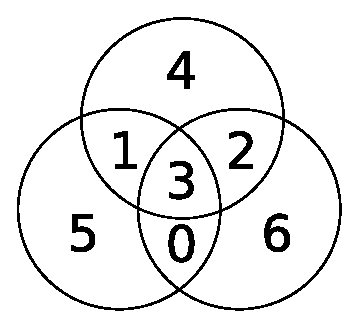
\includegraphics[width=2in,keepaspectratio]{Figures/hammvenn}
\end{center}
\vspace{-4mm}
\caption{Venn diagram representation of the (7,4) binary Hamming code.}
\end{figure}

Let $\mathcal{X}$ be the input alphabet of a channel (assume $\left|\mathcal{X}\right|=q$)
\begin{definition}
A length-$n$ \textbf{code} over the alphabet $\mathcal{X}$ is simply a subset $\mathcal{C}\subseteq\mathcal{X}^{n}$ of all input sequences.
\end{definition}
If a binary code has $M=\left|\mathcal{C}\right|$ codewords, then the code rate is $R=\frac{\log_{2}M}{n}$.
This means we can send $k$ information bits when $M=2^k$.

For example, the binary repeat code of length 5 is defined by $\mathcal{X}=\left\{ 0,1\right\}$ and
\[\mathcal{C}=\left\{ 00000,11111\right\} \subset\left\{ 0,1\right\} ^{5}. \]
Likewise, the binary even parity code of length 3 is
\[ \mathcal{C}=\left\{ 000,110,101,011\right\} \subset\left\{ 0,1\right\} ^{3} . \]

\begin{definition}
The \defn{channel coding}{Hamming distance} $d(\underline{x},\underline{y})$ is equal to the number of places where the vectors differ.
It can be defined mathematically by
\[ d(\underline{x},\underline{y}) = \sum_{i=1}^{n}( 1- \delta_{x_{i},y_{i}}), \]
where $\delta_{a,b}$ is Kronecker delta function
\[\delta_{a,b}=\begin{cases}
0 & \mbox{if }a\neq b\\
1 & \mbox{if }a=b\end{cases}. \]
\end{definition}

The distance between codewords is typically measured with the Hamming distance.
Using this metric, the set $\mathcal{X}^{n}$ forms a discrete metric space
Another important code parameter is the minimum distance $d_{min}$ between any two
codewords is
\[ d_{min}\triangleq\min_{\underline{x},\underline{y}\in\mathcal{C},\underline{x}\neq\underline{y}}d(\underline{x},\underline{y}).\]

\begin{example}[Hamming Code]
The (7,4) binary Hamming Code has $n=7$, $M=16$, and $d_{min}=3$.
The code can be defined in terms of a Venn diagram showing three partially overlapping sets.
Each of the seven subregions represent a code bit and the three circles represent even parity costraints.
Encoding can be done by choosing $x_0,\ldots,x_3$ arbitrarily and then computing the last three parity bits.
Any single error can be corrected by observing each bit error gives a unique pattern of parity violations.
The codewords can be listed as follows:
\[\begin{array}{cccc}
0000000 & 0100110 & 1000011 & 1100101\\
0001111 & 0101001 & 1001100 & 1101010\\
0010101 & 0110011 & 1010110 & 1110000\\
0011010 & 0111100 & 1011001 & 1111111
\end{array} \]
\end{example}

\subsection{Decoding}

Consider the decoding problem for binary codes with $\mathcal{X}=\mathcal{Y}=\left\{ 0,1\right\} $ and $\mathcal{C}\subseteq\mathcal{X}^{n}$.
The channel input is $\underline{x}\in\mathcal{C}$, the received sequence is $\underline{y}$, and the number of errors is $t=d(\underline{x},\underline{y})$
It is not hard to verify that minimum distance decoding, which returns the codeword closest to the channel output, is optimal.
Breaking ties arbitrarily, one can write
\[ \hat{\underline{x}}=\arg\min_{\underline{w}\in\mathcal{C}}d(\underline{w},\underline{y})\]

The following implies that the minimum distance decoder can always correct $t$ errors if $d_{min}\geq2t+1$.
\begin{proposition}
For any received sequence $\underline{y}$, there is at most one codeword $\underline{w}$ such that $d(\underline{y},\underline{w})\leq\frac{d_{min}-1}{2}$.
\end{proposition}
\begin{proof}
Suppose there are codewords $\underline{w},\underline{z}$ where $d(\underline{y},\underline{w})$ and $d(\underline{y},\underline{z})$
are $\leq\frac{d_{min}-1}{2}$.
Then, the triangle inequality implies $d(\underline{w},\underline{z})\!\leq\! d(\underline{y},\underline{w})\!+\! d(\underline{y},\underline{z})\!\leq\! d_{min}-1$ and contradicts the definition of $d_{min}$.
Therefore, if $t\leq\frac{d_{min}-1}{2}$, then $\underline{x}$ is the unique codeword such that $d(\underline{x},\underline{y})\leq\frac{d_{min}-1}{2}$.
\end{proof}

The following allows simultaneous error correction of $t$ errors and detection of $d$ errors.
\begin{proposition}
If $d_{min}\geq t+d+1$ and $d\geq t$, then a single decoder can
both correct $t$ and detect $d$ errors.
\end{proposition}
\begin{proof}
Assume that each codeword is surrounded a inner ball of radius $t$ and an outer ball of radius $d$.
If the received vector is in an inner ball, decode to the codeword at the center.
Otherwise, declare decoding failure.

From the previous result, we see that no two inner balls overlap and that the inner ball of one codeword does not overlap the outer ball of any codeword.
If the number of errors is at most $t$, then received vector will be in the inner ball of the transmitted codeword and will be decoded correctly.
If the number of errors is between $t+1$ and $d$, then received vector will not be in the inner ball of any codeword and failure will be declared.
\end{proof}

\begin{proposition}
If $d_{min}\geq e+1$, then there is a decoder which corrects all patterns of $e$ erasures.
\end{proposition}
\begin{proof}
Make a list of all codewords and then erase any $e$ positions.
Each erasure reduces the minimum distance between any two codewords by at most one.
After $e$ steps, the new $d_{min}\geq e+1-e=1$.
This implies that the codewords, defined by the remaining symbols, are all unique.
\end{proof}

\section{Binary Linear Codes}


\subsection{Basic Properties}

\begin{table}
\begin{center}
\begin{tabular}{c||c|c}
+ & 0 & 1\tabularnewline
\hline
\hline
0 & 0 & 1\tabularnewline
\hline 
1 & 1 & 0\tabularnewline
\end{tabular}~~~\begin{tabular}{c||c|c}
{*} & 0 & 1\tabularnewline
\hline
\hline
0 & 0 & 0\tabularnewline
\hline 
1 & 0 & 1\tabularnewline
\end{tabular}
\caption{The addition and multiplication operations for the binary field.}
\label{tab:BinaryField}
\end{center}
\end{table}

This chapter focuses almost exclusively on binary linear codes, which are the simplest and most important class of error-correcting codes.
The restriction to linear codes can be motivated by two things: simplicity and performance.
We will see later that linear codes are much simpler to describe, encode, and analyze.
Moreover, there are very few cases where non-linear codes are better than linear codes.
So, there is essentially no performance penalty for this simplicity.

Linear codes, like linear algebra, make use of matrices and vectors of elements that can be added, subtracted, multipled, and divided.
A set of numbers which obey all the standard rules of arithmetic is an algebraic object known as a \textbf{field}.
For example, the real and complex numbers are both fields.

There are also fields which have a finite number of elements.
Let $a,d$ be positive integers so that the division of $a$ by $d$ gives the equation $a = dq+r$, where $q$ is quotient and $0\leq r \leq d-1$ is the remainder.
The modulo operation is defined to return the remainder from division and is denoted $r = a \bmod d$.
It turns out that the binary alphabet, $\left\{ 0,1\right\} $, with standard arithmetic ($+,-,*,/$) performed modulo 2 is also a field.
The operations are shown explicitly in Table~\ref{tab:BinaryField}.

For linear algebra over a field, the scalar (i.e., field) operations are used to define vector and matrix operations.
Vector addition is defined element-wise, so that $\left[\underline{x}+\underline{y}\right]_{i}=x_{i}+y_{i}$.
An $(n,k)$ \defn{channel coding}{binary linear code} is $\mathcal{C}\subseteq\left\{ 0,1\right\} ^{n}$ with $\left|\mathcal{C}\right|=2^{k}$ where $\underline{x},\underline{y}\in\mathcal{C}$ implies $\underline{x}+\underline{y}\in\mathcal{C}$
Since $\underline{x}+\underline{x}=\underline{0}$, this implies all zero vector $\underline{0}\in\mathcal{C}$.
For example, the $n=3$ ``even parity'' code is a (3,2) binary linear code with codewords $\mathcal{C}=\left\{ 000,110,101,011\right\} $.

\begin{definition}
The \defn{channel coding}{Hamming weight} $w(\underline{x})$ is the number of non-zero elements in $\underline{x}$ or
\[ w(\underline{x}) = \sum_{i=1}^{n}(1-\delta_{x_i , 0}). \]
For binary vectors, this also implies that the Hamming distance is given by
\[d(\underline{x},\underline{y})=w(\underline{x}-\underline{y}). \]
\end{definition}

Linear codes also have a simplified distance structure.
Instead of considering the minimum distance between all codewords, it suffices to focus only on the all-zero codeword.

\begin{proposition}
The minimum distance of a linear code is given by
\[ d_{min} =\min_{\underline{x}\in\mathcal{C},\underline{x}\neq\underline{0}}w(\underline{x}-\underline{y}). \]
\end{proposition}
\begin{proof}
The linear property of the code allows one to translate computations involving the distance between two codewords to expressions involving the Hamming weight of one codeword.
This gives
\begin{align*}
d_{min}
&\triangleq\min_{\underline{x},\underline{y}\in\mathcal{C},\underline{x}\neq\underline{y}}d(\underline{x},\underline{y}) \\
&=\min_{\underline{x},\underline{y}\in\mathcal{C},\underline{x}\neq\underline{y}}w(\underline{x}-\underline{y}) \\
&=\min_{\underline{x}\in\mathcal{C},\underline{x}\neq\underline{0}}w(\underline{x}-\underline{y}),
\end{align*}
where the last step follows from the fact that
\[ \left\{\underline{x}-\underline{y} \,|\, \underline{x},\underline{y}\in\mathcal{C},\underline{x}\neq \underline{y} \right\}
= \left\{\underline{x}\in\mathcal{C} \,|\, \underline{x}\neq \underline{0} \right\}. \]
\end{proof}

\subsection{Generator and Parity-Check Matrices}

Linear codes can be represented compactly using matrices.
The generator defines the code by allowing one to list all the codewords.

\begin{definition}
The \defn{channel coding}{generator matrix} $\underline{G}$ of an $(n,k)$ binary linear code is a $k\times n$ binary matrix such that all codewords, $\underline{x}\in\mathcal{C}$, can be written as $\underline{u}\cdot\underline{G}=\underline{x}$ for some message vector $\underline{u}\in\left\{ 0,1\right\} ^{k}$.
Therefore, the code is the row space of $\underline{G}$).
\end{definition}

\begin{example}
The generator matrix
\[\underline{G}=\left[\begin{array}{ccccc}
1 & 0 & 1 & 1 & 0\\
1 & 1 & 1 & 0 & 1\end{array}\right] \]
defines the $(5,2)$ code
\[ \mathcal{C} = \left\{ 00000,10110,01011,11101\right\}. \]
Encoding $\underline{u}=[11]$ gives $\underline{u}\cdot\underline{G}=[0\,\,1\,\,0\,\,1\,\,1]$
\end{example}

If $\underline{G}$ has full rank $k$ (over the binary field), then the code has $2^{k}$ distinct codewords.
Otherwise, some non-zero messages encode to the all-zero codeword and there are at most $2^{k-1}$ codewords.

\begin{definition}
The generator matrix is in \defn{channel coding}{systematic form} if $\underline{G}=\left[\underline{P}\,\,\,\underline{I}_{k}\right]$, where $\underline{I}_{k}$ is the $k\times k$ identity matrix.
The matrix $\underline{P}$ is called the \defn{channel coding}{parity generator} of the code because $\underline{u}\cdot\underline{P}$ computes the parity bits for $\underline{u}$.
For a generator matrix in systematic form, the message vector appears in codeword
\[\underline{u}\cdot\underline{G}=\underline{u}\cdot\left[\underline{P}\;\;\underline{I}_{k}\right]=\left[\underline{u}\!\cdot\!\underline{P}\;\;\underline{u}\right]. \]
\end{definition}

The parity-check (PC) matrix defines the code by listing the parity-check equations that each codeword must satisfy.

\begin{definition}
The \defn{channel coding}{parity-check matrix} $\underline{H}$ of an $(n,k)$ binary linear code is an $(n-k)\times n$ binary matrix such that $\underline{x}\cdot\underline{H}^{T}=\underline{0}$ for all $\underline{x}\in\mathcal{C}$.
Therefore, the code is the null space of $\underline{H}$.
\end{definition}

While the generator matrix defines the code and an encoder, the parity-check matrix defines only the code; there is no implied encoder.
There is also a relationship between and generator and parity-check matrix for the same code.
Recall that, for all codewords $\underline{x}$,  there is a message $\underline{u}$ such that $\underline{x}=\underline{u}\cdot\underline{G}$.
This means that $\underline{G}\cdot\underline{H}^{T}=\underline{0}$.

\begin{example}
For the $(5,2)$ code we saw previously, one possible parity-check matrix is
\[ \underline{H}=\left[\begin{array}{ccccc}
1 & 0 & 0 & 1 & 1\\
0 & 1 & 0 & 0 & 1\\
0 & 0 & 1 & 1 & 1\end{array}\right]. \]
Notice that it satisfies $\underline{G}\cdot\underline{H}^{T}=0$ for the previous $\underline{G}$.
\end{example}

In general, we assume that $\underline{H}$ has full rank.
Otherwise, there are redundant constraints and some row can eliminated without changing the code.

A parity-check matrix is in \defn{channel coding}{systematic form} if $H=\left[\underline{I}_{n-k}\,\,\,\,-\underline{P}^{T}\right]$.
When both the generator and parity-check matrices are in systematic form, we can write
\begin{align*}
\underline{G}\cdot\underline{H}^{T}
&=\left[\underline{P}\,\,\,\,\underline{I}_{k}\right]\cdot\left[\underline{I}_{n-k}\,\,\,\,-\underline{P}^{T}\right]^{T} \\
&=\left[\underline{P}\,\,\,\,\underline{I}_{k}\right]\cdot \left[ \begin{array}{c} \underline{I}_{n-k} \\ -\underline{P} \end{array} \right] \\
&=\underline{P}-\underline{P} \\
&=\underline{0}.
\end{align*}

\begin{example}
A \textbf{single parity-check code} is an $(n,n-1)$ binary linear code with parity-check matrix
\[ H=[\underbrace{1,1,\ldots,1}_{n\;\mathrm{times}}]. \]
For all codewords $\underline{x}$, the parity-check constraint $\underline{x}\cdot\underline{H}^{T}=\underline{0}$ implies that $\sum_{i=1}^{n}x_{i}\bmod2=0$ (i.e., the codeword has an even number of ones).
The minimum distance is $d_{min} = 2$ and the generator matrix is given by
\begin{equation*}
G=\left[\begin{array}{ccccc} 1 & 1 & 0 & \cdots & 0 \\ 1 & 0 & 1 & \cdots & 0 \\ \vdots & 0 & \ldots & \ddots & 0 \\ 1 & 0 & 0 & 0 & 1 \end{array}\right].
\end{equation*}
\end{example}

Next, we consider the minimum distance of a code in terms of its generator and parity check matrices.
In general, it is very difficult to compute the minimum distance without enumerating all codewords.
But, one can get upper and lower bounds on the minimum distance much more easily.
In this way, the minimum distance can be found approximately.

Since the minimum distance is equal to the minimum of the Hamming weight overall codewords, it is clearly upper bounded by the Hamming weight of any particular non-zero codeword.
This gives, for any non-zero codewords $\underline{x}$,
\[ d_{min} \leq w(\underline{x}). \]
Likewise, the parity-check matrix can be used to lower bound the minimum distance.
\begin{proposition}
The minimum distance of a code with parity-check matrix
\[\underline{H}=\left[\underline{h}_{1},\underline{h}_{2},\ldots,\underline{h}_{n}\right] \]
is equal to the minimum number of columns that sum to zero or
\[ d_{min}=\min\left\{ w(\underline{x})|\underline{x}\cdot\underline{H}^{T}=\underline{0},\underline{x}\in\left\{ 0,1\right\} ^{n}\backslash\underline{0}\right\}. \]
\end{proposition}
\begin{proof}
Notice that
\[ \underline{x}\cdot\underline{H}^{T}=\sum_{i=1}^n x_{i}\underline{h}_{i}=\sum_{i:x_{i}=1}\underline{h}_{i}, \]
where $\underline{h}_{i}$is the $i$th column of $\underline{H}$.
Therefore, the statement that $\underline{x}\cdot\underline{H}^{T}=\underline{0}$ (i.e., $\underline{x}$ is a codeword) is equivalent to the statement that the sum of $w(\underline{x})$ columns is $\underline{0}$.
Taking the minimum over all non-zero codewords gives the minimum distance.
\end{proof}

One can also bound the minimum distance in terms of error-correction ability.
Recall that a code corrects all error patterns of weight $t$ if and only if $d_{min}\geq2t+1$.
This gives a simple lower bound on the minimum distance.

\begin{example}
Correcting all single errors requires $\frac{d_{min}-1}{2}=1$ or $d_{min}=3$.
Let us try to find the longest code, for a fixed number of parity bits $m$, that corrects all single errors.
In this case, $\underline{H}$ is  matrix with $m$ rows and we can add columns, one at a time, until it is not possible to add a column without losing the ability to correct a single error.
How many columns can we choose?
The maximum value is $n=2^m -1$ and the resuting optimal code is called the binary \defn{channel coding}{Hamming code} of length $n$.
\end{example}

\subsection{Decoding}

Assume a codeword $\underline{x}\in\mathcal{C}$ is transmitted over a channel and $\underline{r}=\underline{x}+\underline{e}$ is received, where $\underline{e}$ is the \textbf{error pattern} with $w(\underline{e})$ errors.
For any received sequence $\underline{r}$, a \textbf{decoder} either returns a codeword $\underline{\hat{x}}=D(\underline{r})$ or declares failure.
The decoded message $\underline{\hat{u}}$ associated with $\underline{\hat{x}}$ is the unique message satisfying $\underline{\hat{x}} = \underline{\hat{u}} \underline{G}$.
A decoder makes
\begin{itemize}
\item a \textbf{block error} (or word error) if $\underline{\hat{x}}\neq\underline{x}$ and $P_{B}$ is used to denote the probability of block error,
\item $b$ \textbf{code bit errors} if $w(\underline{\hat{x}}-\underline{x})=b$ and $P_{b}$ is used to denote the probability that a randomly chosen bit in $\underline{\hat{x}}$ is in error,
\item and $b$ \textbf{message bit errors} if $w(\underline{\hat{u}}-\underline{u})=b$ and $P_{b}$ is used to denote the probability that a randomly chosen bit in $\underline{\hat{u}}$ is in error.
\end{itemize}
From this, we see that the probability of bit error $P_{b}$ can have multiple meanings.
The correct meaning can usually be inferred from the context.
Decoding can also be simplified for linear codes.

\begin{definition}
Let $\underline{s}=\underline{r}\cdot\underline{H}^{T}$ be the \textbf{syndrome} of the received vector $\underline{r}$.
\end{definition}
It turns out that $\underline{s}$ depends only on the error pattern.
Since $\underline{x}\in\mathcal{C}$, we have
\[ \underline{s}=\underline{r}\cdot\underline{H}^{T}=(\underline{x}+\underline{e})\cdot\underline{H}^{T}=\underline{x}\cdot\underline{H}^{T}+\underline{e}\cdot\underline{H}^{T}=\underline{e}\cdot\underline{H}^{T}. \]

A \defn{channel coding}{syndrome decoder} $\underline{\hat{e}}=D_{s}(\underline{s})$ maps the syndrome $\underline{s}$ to an estimated error pattern $\underline{\hat{e}}$.
Let us define the equivalence relation $\sim$ by $\underline{x}\sim\underline{y}$ iff $\underline{x}\cdot\underline{H}^{T}=\underline{y}\cdot\underline{H}^{T}$.
This means that two binary vectors are equivalent if they have the same syndrome.
A syndrome decoder can be designed correct exactly one error pattern in each equivalence class.
The best choice for correction is the most-likely error pattern in that equivalence class.
For most channels, these vectors are chosen to be the minimum weight vector in the equivalence class.

The \defn{channel coding}{standard array} is way of listing all vectors of length-$n$ that exposes the connectiion between syndromes, codewords, and error correction.
In general, it is a $2^{n-k}\times 2^k$ table that contains each length-$n$ binary vector exactly once.
The main idea behind this table is that, when one chooses to correct a particular error pattern, the decoder is automatically defined for all received sequences equal to that error pattern plus a codeword.
Of course, this limits one's ability choose correctable error patterns.


Each row is indexed by a syndrome $\underline{s}$ and contains all binary vectors $\underline{x}$ that satisfy the equation $\underline{s}=\underline{x}\cdot\underline{H}^{T}$.
The first row is reserved for $\underline{s}=\underline{0}$ and contains the all-zero codeword $\underline{c}_1$ in the first column followed the remaining codewords $\underline{c}_2,\ldots,\underline{c}_{2^k}$ in any order.
The first column contains the correctable error patterns $\underline{e}_1 ,\ldots, \underline{e}_{2^{n-k}}$ where $\underline{e}_1$ is the all-zero sequence.
The row-$i$ column-$j$ entry always contains $\underline{e}_i + \underline{c}_j$, and is therefore defined by the first row and first column of the table.
The column associated with a particular codeword can be seen as all the received vectors that will be decoded to that codeword.


Using the parity-check matrix for our $(5,2)$ our example code, the process is as follows
\begin{enumerate}
\item Start with 8 by 5 table and list the zero syndrome and all codewords on first row
\item Pick a minimum weight vector of length $n$ that is not already in table and compute its syndrome
\item Add a new row by writing syndrome followed by the minimum weight vector plus each codeword
\item Repeat from step 2 until table is complete.
\end{enumerate}
The resulting standard array is
\begin{center}
\begin{tabular}{|c||c|c|c|c|}
\hline 
syn\textbackslash cw &  00000 & 10110 & 01011 & 11101\tabularnewline
\hline
\hline 
100 & 10000 & 00110 &  & 01101\tabularnewline
\hline 
010 & 01000 &  & 00011 & \tabularnewline
\hline 
001 & 00100 & 10010 &  & 11001\tabularnewline
\hline 
101 & 00010 &  & 01001 & \tabularnewline
\hline 
111 & 00001 & 10111 &  & 11100\tabularnewline
\hline 
110 & 11000 & 01110 & 10011 & \tabularnewline
\hline 
011 & 01100 & 11010 &  & 10001\tabularnewline
\hline
\end{tabular}
\end{center}
To see if you understand this example, try filling in the missing entries.
One can prove that this process always enumerates all $2^{n}$ binary vectors, so you can test your answers by checking if all binary vectors appear in the table exactly once.

\begin{example}
To see syndrome decoding in action, let $\underline{x}=10110$ and $\underline{e}=11000$.
Then, $\underline{r}=01110$ and $\underline{s}=110$.
Looking in the syndrome table, we find that $\underline{\hat{e}}=11000$ and $\underline{\hat{x}}=10110$.
\end{example}

\subsection{Manipulating Linear Codes}

It follows from linear algebra that any $\underline{G},\underline{H}$ can be put in systematic form using elementary row operations and (possibly) a column permutation.
For the parity-check matrix $H$, the basic idea is to use elemtary row operations to form an identity matrix in the first few columns (i.e., put it in reduced row-echelon form).
For the generator matrix $G$, elementary row operations are used to form an identity matrix in the last few columns.
Sometimes an identity cannot be formed in the desired columns and a column permutation is required to complete the process.
For this reason, two codes are called \textbf{equivalent} if and only if they differ only in the order of the code symbols.

\begin{definition}
For a matrix, an \textbf{elementary row operation} is any one of the following operations:
\begin{enumerate}
\item interchaging any two rows,
\item scaling any row by a non-zero constant,
\item and adding a multiple of one row to another row.
\end{enumerate}
\end{definition}

\begin{example}
In this example, we consider a parity-check matrix
\[ \underline{H} =\left[\begin{array}{cccccc}
1 & 1 & 0 & 1 & 0 & 0\\
0 & 1 & 1 & 0 & 1 & 0\\
1 & 1 & 0 & 0 & 1 & 1\end{array}\right] \]
that requires a column permutation for systematic form.
Let us put $\underline{H}$ is reduced row-echelon form and then find a column permutation to achieve an identity in the first few rows.
The first step gives
\[ \underline{H} \rightarrow\left[\begin{array}{cccccc}
1 & 1 & 0 & 1 & 0 & 0\\
0 & 1 & 1 & 0 & 1 & 0\\
0 & 0 & 0 & 1 & 1 & 1\end{array}\right]\rightarrow\left[\begin{array}{cccccc}
1 & 0 & 1 & 1 & 1 & 0\\
0 & 1 & 1 & 0 & 1 & 0\\
0 & 0 & 0 & 1 & 1 & 1\end{array}\right]
\rightarrow\left[\begin{array}{cccccc}
1 & 0 & 1 & 0 & 0 & 1\\
0 & 1 & 1 & 0 & 1 & 0\\
0 & 0 & 0 & 1 & 1 & 1\end{array}\right], \]
and a column permutation gives
\[ \tilde{\underline{H}}=\left[\begin{array}{cccccc}
1 & 0 & 0 & 1 & 0 & 1\\
0 & 1 & 0 & 1 & 1 & 0\\
0 & 0 & 1 & 0 & 1 & 1\end{array}\right]. \]
Now, we can compute parity generator and generator associated with $\tilde{\underline{H}}$ to get
\[ \tilde{\underline{P}}=\left[\begin{array}{ccc}
1 & 1 & 0\\
0 & 1 & 1\\
1 & 0 & 1\end{array}\right] \quad 
\tilde{\underline{G}}=\left[\begin{array}{cccccc}
1 & 1 & 0 & 1 & 0 & 0\\
0 & 1 & 1 & 0 & 1 & 0\\
1 & 0 & 1 & 0 & 0 & 1\end{array}\right]. \]
Finally, reversing the column permutation gives, for the original code, a generator
\[\underline{G}=\left[\begin{array}{cccccc}
1 & 1 & 1 & 0 & 0 & 0\\
0 & 1 & 0 & 1 & 1 & 0\\
1 & 0 & 0 & 1 & 0 & 1\end{array}\right]  \]
that contains an identity in a subset of its columns.
\end{example}

\section{Performance Analysis}

Consider an $(n,k)$ binary code of rate-$R$ with $d_{min} \geq 2t^* + 1$ and a decoder that corrects all error patterns of weight at most $t^*$.
It is relatively easy to upper bound the probability of block error when this code and decoder are used on a BSC, because a block error cannot occur unless there are more than $t^*$ errors.
This gives
\[ P_{B}\leq1-\sum_{i=0}^{t^*}{n \choose i}p^{i}(1-p)^{n-i}=\sum_{i=t^*+1}^{n}{n \choose i}p^{i}(1-p)^{n-i}. \]
If the code bits are transmitted over an AWGN channel using BPSK followed by a hard-decision detector, then we also have
\[ p= Q\left( \sqrt{\frac{2 E_s}{N_0}} \right) = Q\left( \sqrt{\frac{2 R  E_b}{N_0}} \right). \]
The latter expression allows us to make relatively fair comparisons between coding systems with different rates.
 
For syndrome decoding, one can compute the probability of block error (including decoding failure) exactly by observing that the decoder only returns the correct codeword if the error vector is a coset leader.
In this case, we can define $A_h$ be the number of coset leaders with Hamming weight $h$ and write
\[ P_{B} = 1-\sum_{h=0}^{n} A_h p^h (1-p)^{n-h}. \]

\section{Cyclic Codes}

\subsection{Basic Properties}
In this section, we consider a subset of linear codes which have even more algebraic structure.
A cyclic (or circular) shift of a vector is another vector with the same elements in the same order, but starting from an different index.
For example, the left circular shift of $(x_0,x_1,\ldots,x_{n-1})$ by 1 position gives the vector $(x_{n-1},x_0,x_1,\ldots,x_{n-2})$.

\begin{definition}
A \defn{channel coding}{cyclic code} is a linear code where any cyclic shift of a codeword is also a codeword.
\end{definition}

\begin{example}
Consider the $(7,3)$ binary linear code whose 8 codewords are
\[ \mathcal{C} = \left\{
0000000,
1011100,
0101110,
1110010,
0010111,
1001011,
0111001,
1100101
\right\}. \]
Since all non-zero codewords are circular shifts of a single codeword, it is a cyclic code.
Its cyclic structure can also be exposed by choosing the generator matrix to be
\[ \underline{G} = \left[ \begin{array}{ccccccc}
1 & 0 & 1 & 1 & 1 & 0 & 0 \\
0 & 1 & 0 & 1 & 1 & 1 & 0 \\
0 & 0 & 1 & 0 & 1 & 1 & 1 \end{array} \right] \]
and the parity-check matrix to be
\[ \underline{H} = \left[ \begin{array}{ccccccc}
1 & 1 & 0 & 1 & 0 & 0 & 0 \\
0 & 1 & 1 & 0 & 1 & 0 & 0 \\
0 & 0 & 1 & 1 & 0 & 1 & 0 \\
0 & 0 & 0 & 1 & 1 & 0 & 1 \end{array} \right]. \]
\end{example}

The benefits of cyclic codes follow largely from a close conection to polynomial arithmetic.
This allows the encoding and decoding of cyclic codes to make use of efficient algorithms and hardware for polynomial arithmetic.
Consider an $(n,k)$ cyclic code and assume each codeword vector $\underline{c}=(c_0,c_1,\ldots,c_{n-1})$ and message vector $\underline{m}=(m_0,m_1,\ldots,m_{k-1})$ is associated with a polynomial
\[ c(x) = \sum_{i=0}^{n-1} c_i x^i \quad \quad  m(x) = \sum_{i=0}^{k-1} m_i x^i. \]
It turns out that every $(n,k)$ cyclic code is uniquely defined by its generator polynomial $g(x)$, which allows all codewords $c(x)=m(x)g(x)$ to be generated by multiplication with some message polynomial $m(x)$.
The generator polynomial for the code in the previous example is $g(x) = 1 + x^2 + x^3 + x^4$.

Before proceeding any further, we must define a few mathematical terms asociated with polynomial arithmetic.
The \textbf{degree} of a polynomial $c(x)$, denoted $\deg\left( c(x) \right)$, is the maximum power of $x$ that appears in the polynomial.
For the example $g(x)$, we have $\deg \left( g(x) \right) = 4$.
In fact, for all $(n,k)$ cyclic codes, we have
$\deg \left( c(x) \right) \leq n-1$,
$\deg \left( m(x) \right) \leq k-1$, and
$\deg \left( g(x) \right) = n-k$.

For a polynomial $a(x)$ and a divisor $d(x)$, the \textbf{remainder} $r(x)$ and \textbf{quotient} $q(x)$  are uniqely defined by $\deg\left( r(x) \right) < \deg \left(d(x) \right)$ and
\[ \frac{a(x)}{d(x)} = q(x) + \frac{r(x)}{d(x)}. \]
In discrete mathematicss, the \defn{channel coding}{modulo polynomial} operation
\[ a(x) \bmod d(x) = r(x) \]
is used to compactly represent the remainder of division by $d(x)$.
\begin{proposition}
For an $(n,k)$ cyclic code defined by its generator polynomial $g(x)$, the parity-check polynomial $h(x)$ is defined uniquely by $g(x)h(x)=x^n - 1$ and satisfies
\[ h(x)c(x) = 0 \bmod x^n - 1, \]
for all codeword polynomials $c(x)$.
\end{proposition}
\begin{proof}
One can prove this statement by observing that $c(x)=m(x)g(x)$ for some $m(x)$ and therefore
\[ h(x)c(x) = m(x)g(x)h(x) = m(x)(x^n - 1). \]
Since $x^n -1$ divides $h(x)c(x)$ without remainder, the result follows.
\end{proof}
The parity-check polynomial for the code in the previous example is $h(x) = 1 + x^2 + x^3$.

In general, the generator matrix of an $(n,k)$ cyclic code with generator $g(x)=g_0 + g_1 x + g_2 x^2 + \cdots g_{n-k} x^{n-k}$ can be written in the form
\[ \underline{G} = \left[ \begin{array}{ccccccc}
g_0 & g_1 & \cdots & g_{n-k} & 0 & 0 & 0 \\
0 & g_0 & g_1 & \cdots & g_{n-k} & 0 & 0 \\
\vdots & \vdots & \ddots & \ddots & \ddots & \ddots & 0 \\
0 & 0 & 0 & g_0 & \cdots & g_{n-k-1} & g_{n-k} \end{array} \right]. \]
Likewise, the parity-check polynomial $h(x) = h_0 + h_1 x + h_2 x^2 + \cdots h_{k} x^k$ gives rise to a parity-check matrix of the form
\[ \underline{H} = \left[ \begin{array}{ccccccc}
h_k & h_{k-1} & \cdots & h_0 & 0 & 0 & 0 \\
0 & h_k & h_{k-1} & \cdots & h_0 & 0 & 0 \\
\vdots & \vdots & \ddots & \ddots & \ddots & \ddots & 0 \\
0 & 0 & 0 & h_k & \cdots & h_1 & h_0 \end{array} \right]. \]

The encoder mapping $\underline{c} = \underline{m} \, \underline{G}$ is actually identical to the encoder mapping $c(x) = m(x) g(x)$.
If the rows and columns of $\underline{G}$ are numbered from zero, then this can be seen by associating the $i$th row of $\underline{G}$ with $x^i$ and the $j$th column of $\underline{G}$ with $x^j$.
Observing that $[\underline{G}]_{ij} = g_{j-i}$ for $i \leq j \leq n-1$ and 0 otherwise, we find that
\begin{align*}
c(x)
&= \sum_{j=0}^{n-1} x^j c_j 
= \sum_{j=0}^{n-1} x^j \sum_{i=0}^{k-1} m_i [\underline{G}]_{ij} 
= \sum_{j=0}^{n-1} x^j \sum_{i=0}^{k-1} m_i g_{j-i} \\
&= \sum_{i=0}^{k-1} m_i x^i \sum_{j=i}^{n-1} x^{j-i} g_{j-i} 
= \sum_{i=0}^{k-1} m_i x^i g(x) 
= m(x) g(x).
\end{align*}

\begin{example}
The binary Hamming codes are a family of $(n,k)$ cyclic codes, that can correct all single errors, with $n=2^r - 1$ and $k=n-r$.
The generator polynomials for $k=3,4,5$ are given by
\begin{align*}
(7,4) & \quad \quad g(x) = 1+x^2+x^3 \\
(15,11) & \quad \quad g(x) = 1+x^3+x^4 \\
(31,26) & \quad \quad g(x) = 1+x^3+x^5.
\end{align*}
\end{example}

\subsection{Systematic Encoding}

For cyclic codes, the basic encoding process $c(x)=m(x)g(x)$ does not provide systematic encoding.
One can overcome this limitation by observing that $c(x) \bmod g(x) = 0$ for all codewords.
Using this equation instead, one can choose the codeword have the format
\[ c(x) = p(x) + x^{n-k} m(x), \]
where the message $m(x)$ appears as the last $k$ bits in the codeword and the parity polynomial $p(x)=p_0 + p_1 x + \cdots p_{n-k-1} x^{n-k-1}$ has degree $\deg\left( p(x)\right) = n-k-1$.
Applying the modulo $g(x)$ operation to both sides of this equation shows that
\[ 0 = c(x) \bmod g(x) = p(x) \bmod g(x) + x^{n-k} m(x) \bmod g(x). \]
Solving for $p(x)$ gives
\[ p(x) = - x^{n-k} m(x) \bmod g(x), \]
where $p(x) = p(x) \bmod g(x)$ follows from the fact that $\deg\left( p(x)\right) < \deg\left( g(x)\right)$.
For cyclic codes, this process defines the standard \defn{channel coding}{systematic encoder} used in practice.
It turns out that that  $p(x)$ can be calculated efficiently using a shift register circuit.
So, systematic encoders for cyclic codes are easy to implement in practice.

\begin{example}
Consider our example $(7,3)$ code with $g(x) = 1 + x^2 + x^3 + x^4$.
The message $\underline{m} = [0\;1\;1]$ is associated with the message polynomial $m(x) = x+x^2$ and the systematic encoding equation says that
\[ p(x) = - x^4 m(x) \bmod g(x) = -x^5 - x^6 \bmod 1+x^2 + x^3 + x^4. \]
To compute $p(x)$, we proceed by using polynomial long division
\begin{center}
\polylongdiv{-x^5 - x^6}{x^4+x^3+x^2+1}
\end{center}
This implies that $p(x) = x^3+1$ and $c(x) = 1+x^3 + x^5 + x^6$.
One can verify that this is a codeword by observing that $(1+x^2)(1+x^2+x^3+x^4)\bmod 2 = 1+x^3+x^5+x^6$.
\end{example}

\subsection{Cyclic Redundancy Check}

A \defn{channel coding}{cyclic redundancy check} (CRC) code calculates its check bits using a process very similar to the systematic encoding of cyclic codes.
The main difference is that the message polynomial $m(x)$ is not constrained to be $k$ bits in length and it is not multiplied by $x^{n-k}$ before the modulo operation.
Let $g(x)$ be the CRC polynomial and $m(x)$ be the message polynomial, then the CRC encoder generates the check polynomial
\[ p(x) = m(x) \mod g(x). \]
Since  $\deg \left(p(x)\right) < \deg \left(g(x)\right)$, the resulting check sequence is represented by exactly $\deg \left(g(x)\right)-1$ bits.
Many of the CRCs defined in standards (or commonly used in practice) have subtle variations such as
\begin{itemize}
\item extra bits are appended to the start or end of the message,
\item the shift register state is initialized to a non-zero value,
\item the message sequence is XOR'd with a known sequence before division,
\item and the bit (or byte) ordering may differ between standards.
\end{itemize}

In most specifications, the CRC polynomial is not described as a polynomial but instead given as the hexadecimal value of the binary representation of $g(x)$.
Moreover, the topmost bit is not included in this value because the length is know and it must a 1.
\begin{example}
The standard unix CRC32 polynomial is often listed in hexadecimal as \texttt{04C11DB7}.
Writing this in binary gives
\[ 0000\;0100\;1100\;0001\;0001\;1101\;1011\;0111. \]
Counting from the right (i.e., the LSB), we find ones in the positions
\[ 0,1,2,4,5,7,8,10,11,12,16,22,23,26. \]
Therefore, it follows that
\[ g(x) = x^{32} + x^{26} + x^{23} + x^{22} + x^{16} + x^{12} + x^{11} + x^{10} + x^8 + x^7 + x^5 + x^4 + x^2 + x + 1.\]
Notice the $x^{32}$ is added based on the known length of the CRC and is not described by the hexadecimal value.
\end{example}

The CRC32 algorithm prepends the data sequence by 32 ones, performs the modulo, and then inverts the resulting parity sequence.
The ASCII sequence ``123456789" has the hexadecimal representation \texttt{31\,32\,33\,34\,35\,36\,37\,38\,39} and is commonly used to test CRC implementations.
For this sequence, the correct CRC result, in hexadecimal, is \texttt{CBF43926}.


\iffalse
\begin{tabular}{ccccccc}
& $x^3$ & $+x^2$ & $+x$ & $+1$ & & \\
$ x^4 + x^3 + x^2 + 1 $ & $x^6$ & $+x^5$ & $+0x^4$ & $+x^3$ & 
\begin{equation*}

each codeword is a 
Define all polynomials

careful of syndrome definition: depends on H matrix

discuss root structure

generator/parity check matrix from polynomial mult

general, primitive for all cyclic codes

\fi

%\chapter{Waveform Communication}
\label{chapter:ContinuousTimeComm}

In Chapter~\ref{chapter:DiscreteTimeComm}, we introduced digital communication using a discrete-time model that allowed us to neglect the details of the more realistic continuous-time model.
The goal of this chapter is to delve into the details of waveform-based communication and see that the discrete-time model can be derived from the continuous-time model under some conditions.
The \defn{communication}{waveform channel} defines the probabilistic mapping between the deterministic channel input waveform $s(t)$ and the random-process $R(t)$ observed at the output of the channel.
The basic model is that $R(t) = s(t) + N(t)$, where $N(t)$ is Gaussian white-noise random process with autocorrelation function $R_N (\tau) = \delta(\tau) N_0 / 2$.
%In some cases, the channel will also act as a linear filter and produce $R(t) = h(t) * s(t) + N(t)$, where $h(t)$ is the channel response.

\begin{figure}
\begin{center}
\begin{psfrags}
\psfrag{c}[c]{Channel}
\psfrag{x}[l]{$s(t)$}
\psfrag{n}[l]{$N(t)$}
\psfrag{r}[l]{$R(t)$}
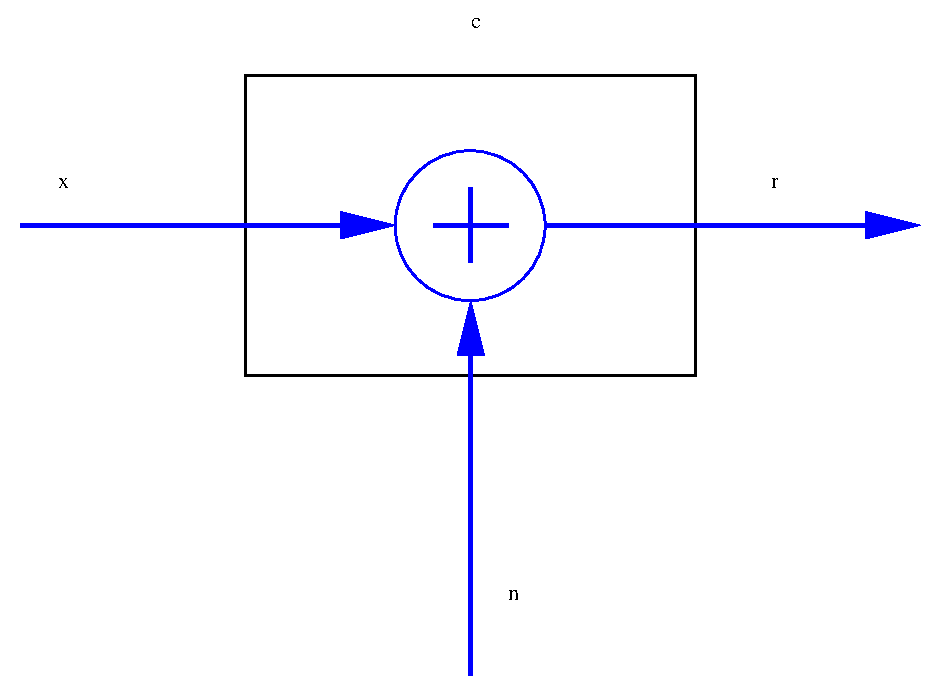
\epsfig{file=Figures/channel.eps,width=6.5cm}
\end{psfrags}
\end{center}
\caption{Block diagram of a basic waveform channel for input signal $s(t)$, noise process $N(t)$, and received signal $R(t)$.}
\end{figure}

\iffalse
\emph{Modulation} is the process by which a string of bits is converted into a signal suitable for transmission over a communication channel.
\emph{Demodulation} is the reverse operation at the destination where the information symbols are extracted from the received signal.
The shapes of the waveforms employed to create the transmitted signal are critical to the overall performance and operation of the system.
In many implementations, a high-frequency sinusoid is used, in addition to baseband pulse waveforms, as carrier to center the baseband signal at its intended frequency.
We initiate our study of modulation and demodulation with baseband signals; advanced considerations associated with carrier sinusoids and bandpass processes will be explored later.

Let $\{ s_k \in \{ 0, 1 \}^b \}$ be a sequence of binary symbols to be transmitted to a destination, and let $f : \{ 0, 1 \}^b \mapsto \mathbb{R}$ be an invertible function that takes a string of $b$ bits as input, and gives a real number as output, with $u_k = f(s_k)$.
Suppose further that several distinct waveforms are available at the transmitter, which we denote by $\{ \phi_k (t) \}$.
We study communication systems that modulate binary symbols in two steps.
First, a collection of binary data $\{ s_k \}$ is converted into a string of real numbers $\{ u_k \}$ using function $f(\cdot)$.
Next, these real numbers are used to form a transmission signal by creating a weighted linear combination of the basis functions,
\begin{equation*}
u(t) = \sum_k u_k \phi_k(t) .
\end{equation*}
This procedure provides a simple framework to transition back and forth between a digital sequence and the corresponding modulated signal.
At the destination, the sequence of binary symbols is demodulated by passing the received signal through linear time-invariant filters, and then mapping the resulting real number to one of the possible $b$-bit messages.
\fi

\section{A Single Digital Symbol}

Suppose that one would like to send a single digital symbol taking $M$ different values to a receiver through a waveform channel.
Then, one can associate a waveform $s_m (t)$ with each symbol $m=1,\ldots,M$ and transmit the waveform assigned with the desired message.
For mathematical convenience, we assume that the energy integral exists and is finite for each waveform.

The demodulation process is based on mathematical operation, known as an inner product, that maps any two signals to a complex number.
The \defn{communication}{inner product} $\langle s(t) , r(t) \rangle$ between the signals $s(t)$ and $r(t)$ is defined by
\begin{equation*}
\left\langle s (t), r^* (t) \right\rangle
= \int_{-\infty}^{\infty} s(t) r^* (t) dt,
\end{equation*}
where $r^* (t)$ is the complex conjugate of $r(t)$.
This is the same as the cross-correlation between $r(t)$ and $s(t)$ evaluated at lag-time 0.
Mathematically, we are treating the set of all finite-energy signals as a \defn{communication}{vector space} and using this inner product to define distances and angles in this space.
The energy (or length squared) of a signal $s(t)$ is given by
\[ \int_{-\infty}^{\infty} \left| s(t) \right|^2 dt = \langle s(t),s(t) \rangle. \]
Two signals $s_1 (t),s_2 (t)$ are said to be \defn{communication}{orthogonal} if $\langle s_1(t),s_2 (t)\rangle = 0$.
A signal $s(t)$ is said to be \textbf{normalized} if $\langle s(t),s(t) \rangle = 1$.
A set of signals is said to be \textbf{orthonormal} if every signal in the set is orthogonal to every other signal in the set and all signals in the set are normalized.
The set of all linear combinations of signal waveforms is called the \defn{communication}{signal space}.

\subsection{Orthonormal Waveforms}
The simplest scenario occurs when the set of signal waveforms $\{ s_1 (t), \ldots , s_M (t) \}$ is orthonormal.
In this case, one can demodulate the received signal $R(t)$ by computing
\[ R_j = \langle R(t), s_j (t) \rangle, \]
for each $j=1,\ldots,M$.
This is the same as correlating the received signal with each of the transmitted waveforms.
Due to the noise process, the resulting values $R_1 , \ldots, R_M$ are Gaussian random variables.
Their expected values depend on which waveform was actually transmitted.
If $s_m (t)$ was transmitted, then $R(t) = s_m(t) + N(t)$, $E[R(t)] = s_m(t)$, and we have
\begin{align*}
E \left[R_j \right]
&= E \left[ \int_{-\infty}^{\infty} R(t) s_j^* (t) dt \right] \\
&= \int_{-\infty}^{\infty} E \left[ R(t) \right] s_j^* (t) dt \\
&= \int_{-\infty}^{\infty} s_m (t) s_j^* (t) dt \\
&= \delta_{m,j}.
\end{align*}

The random variables $R_1, \ldots , R_M$ also have some other nice properties.
They are uncorrelated because the the waveforms are orthogonal and they have variance $N_0  / 2$ because the waveforms are normalized.
Proving this statement will be left as a homework exercise.

This transforms the waveform detection problem into a detection problem for a length-$M$ vector of Gaussian random variables.
If $s_m (t)$ was transmitted, then the mean of the random vector is the unit vector with a one in the $m$th position.
Let $(r_1, \ldots, r_M)$ be the realization of the random vector $(R_1,\ldots,R_M)$.
Then, based on the techniques from Chapter~\ref{chapter:DiscreteTimeComm}, we know that the maximum-likelihood decision rule chooses the symbol whose unit vector is closest to $(r_1,\ldots,r_M)$ in Euclidean distance.
This implies that we should choose the signal $s_{m^*}(t)$ if
\[ \sum_{i=1}^M (r_i - \delta_{m^*,i})^2 \leq \sum_{i=1}^M (r_i - \delta_{m,i})^2 \quad \mathrm{for}\; m=1,\ldots,M. \]
Expanding both sides of this equation shows that this is equivalent to
\[ r_{m^*} \geq r_m \quad \mathrm{for}\; m=1,\ldots,M. \]
This whole process is known as a correlation-based receiver.


\begin{example}[Frequency-Shift Keying] \label{example:TSpacedTruncatedSinusoids}
For a fixed time-interval $T$, consider the collection of waveforms given by
\begin{equation*}
s_m(t) = \frac{1}{\sqrt{T}} e^{2 \pi i \frac{m}{T} t} \mathrm{rect} \left( \frac{t}{T} \right) .
\end{equation*}
for $m = 1, \ldots, M$.
This set of waveforms is known as $M$-ary frequency-shift keying (or $M$-FSK).
We wish to show that these waveforms are orthonormal.

To prove that they are orthogonal, we consider the inner product of $s_m(t)$ and $s_n(t)$ when $m \neq n$,
\begin{equation*}
\begin{split}
\left\langle s_m (t), s_n (t) \right\rangle
&= \int_{\mathbb{R}} s_m (t) s_n^* (t) dt 
= \frac{1}{T} \int_{-\frac{T}{2}}^{\frac{T}{2}}
e^{2 \pi i \frac{m}{T} t} e^{- 2 \pi i \frac{n}{T} t} dt \\
&= \frac{1}{T} \int_{-\frac{T}{2}}^{\frac{T}{2}}
e^{2 \pi i \frac{(m-n)}{T} t} dt
= 0 .
\end{split}
\end{equation*}
Next, we show that these basis elements have unit energy,
\begin{equation*}
\begin{split}
\left\| s_m(t) \right\|^2
&= \int_{\mathbb{R}} s_m (t) s_m^* (t) dt 
= \frac{1}{T} \int_{-\frac{T}{2}}^{\frac{T}{2}}
e^{2 \pi i \frac{m}{T} t} e^{- 2 \pi i \frac{m}{T} t} dt \\
&= \frac{1}{T} \int_{-\frac{T}{2}}^{\frac{T}{2}} dt
= 1 .
\end{split}
\end{equation*}
\end{example}

\subsection{General Waveforms}

When the signal waveforms are not orthonormal, the detection problem is solved most easily by constructing a set of orthonormal basis vectors for the signal space.
In general, this can be accomplished by applying the Gram-Schmidt orthogonalization process to the signal waveforms.
Rather than focusing on this process, we assume that $\{ \phi_1 (t), \ldots , \phi_N (t) \}$ is an orthonormal set of waveforms such that the coefficients $a_{m,k}$ allow us to write
\[ s_m (t) = \sum_{k=1}^N a_{m,k} \phi_k (t). \]
This implies that the orthonormal set spans the signal space.

In this case, the received signal $R(t)$ can be demodulated by computing
\[ R_j = \langle R(t), \phi_j (t) \rangle, \]
for each $j=1,\ldots,N$.
This is the same as correlating the received signal with each of the basis waveforms.
Again, the noise process implies that $R_1 , \ldots, R_N$ are Gaussian random variables whose means are determined by which waveform was actually transmitted.
For $j=1,\ldots,N$, the noise component of $R_j$ is independent of the transmitted signal, and is given by
\[ N_j = \langle N(t), \phi_j (t) \rangle = \int_{-\infty}^{\infty} N(t) \phi_j^* dt. \]
Therefore, $R_j = E[R_j] + N_j$ and, assuming $s_m (t)$ was transmitted, the mean is given by
\begin{align*}
E \left[R_j \right]
&= E \left[ \int_{-\infty}^{\infty} R(t) \phi_j^* (t) dt \right] \\
&= \int_{-\infty}^{\infty} E \left[ R(t) \right] \phi_j^* (t) dt \\
&= \int_{-\infty}^{\infty} s_m (t) \phi_j^* (t) dt \\
&= \int_{-\infty}^{\infty} \left( \sum_{k=1}^N a_{m,k} \phi_k (t) \right) \phi_j^* (t) dt \\
&= \sum_{k=1}^N a_{m,k} \delta_{k,j} dt \\
&= a_{m,j}. 
\end{align*}

Again, we have transformed the waveform detection problem into a detection problem for a vector of Gaussian random variables.
In this case, however, there are $M$ different mean vectors of dimension $N$.
Let $(r_1, \ldots, r_N)$ be the realization of the random vector $(R_1,\ldots,R_N)$.
Based on the techniques from Chapter~\ref{chapter:DiscreteTimeComm}, the maximum-likelihood decision rule chooses the symbol $m^*$ whose coordinate vector $(a_{m^*,1},\ldots. a_{m^*,N})$ is closest to $(r_1,\ldots,r_N )$ in Euclidean distance.
This implies that we should choose the signal $s_{m^*}(t)$ if
\[ \sum_{i=1}^N (r_i - a_{m^*,i})^2 \leq \sum_{i=1}^N (r_i - a_{m,i})^2 \quad \mathrm{for}\; m=1,\ldots,M. \]

This approach can be seen as first projecting the infinite-dimensional received waveform onto the finite-dimensional signal-subspace and then using the optimal detector assuming only the projection was observed.
This overall approach is optimal only if the projection is a \textbf{sufficient statistic} for maximum-likelihood decision problem.
While this is indeed true, we disregard this detail for now.

\begin{figure}
\begin{center}
\begin{psfrags}
\psfrag{p1}[l]{$\phi_1(t)$}
\psfrag{p2}[l]{$\phi_2(t)$}
\psfrag{p3}[l]{$\phi_{N-1}(t)$}
\psfrag{p4}[l]{$\phi_N(t)$}
\psfrag{i}[c]{$\int_{0}^T (\cdot) dt$}
\psfrag{r}[l]{$r(t)$}
\psfrag{r1}[l]{$r_1$}
\psfrag{r2}[l]{$r_2$}
\psfrag{r3}[l]{$r_{N-1}$}
\psfrag{r4}[l]{$r_N$}
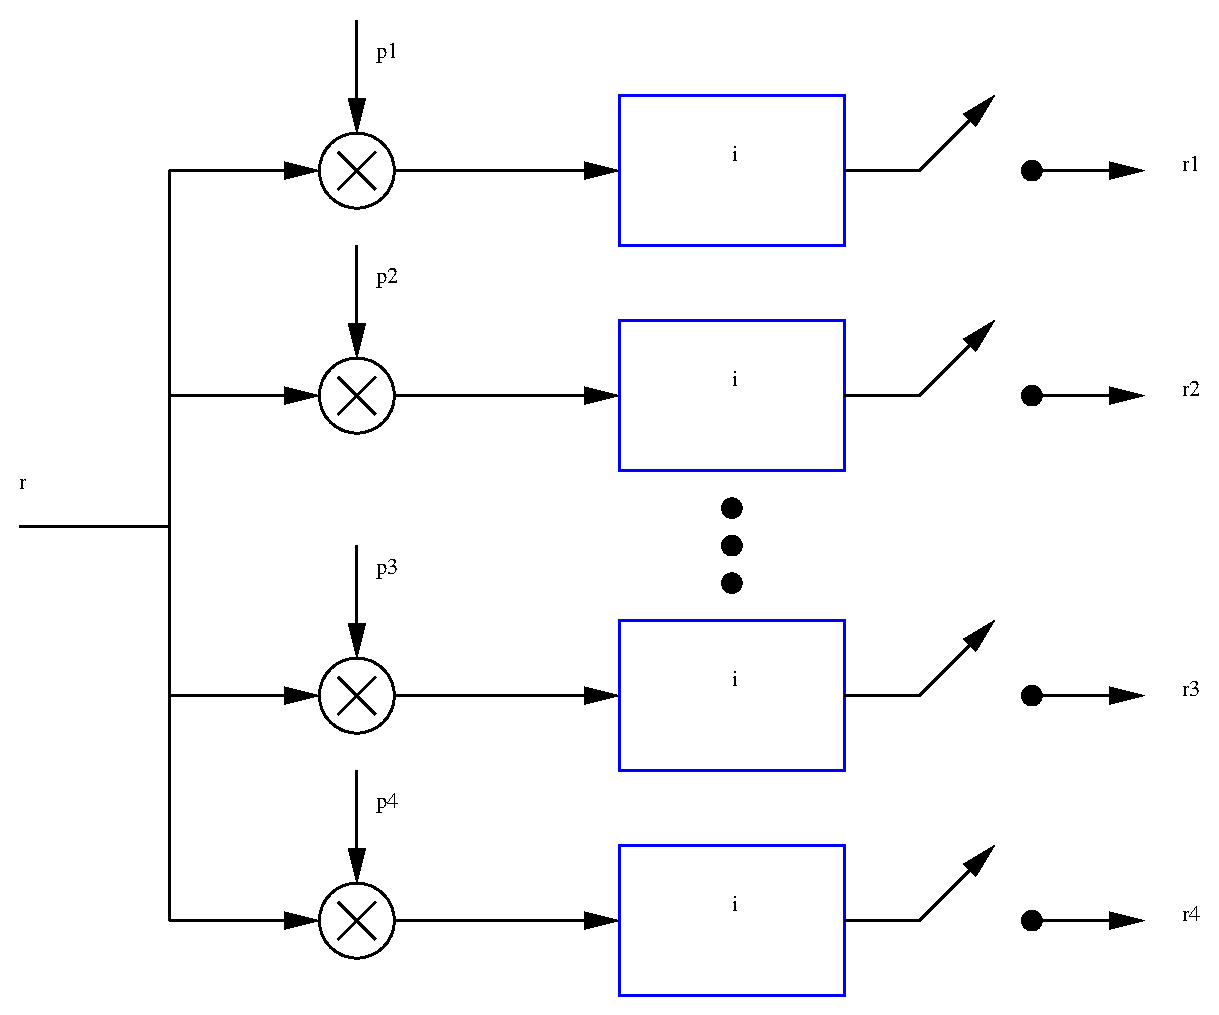
\epsfig{file=Figures/correlator.eps,width=8cm}
\end{psfrags}
\end{center}
\caption{For a particular realization $r(t)$ of the received signal, the projection $(r_1,\ldots,r_N)$ onto the signal-space basis vectors can be computed by a bank of correlators.}
\end{figure}

\subsection{The Matched Filter}

Let $s(t)$ be a finite-energy signal and $R(t)=s(t)+N(t)$ be the received waveform.
Suppose that the receiver computes $R = \langle R(t), z(t) \rangle$ with an arbitrary finite-energy signal $z(t)$.
One's ability to detect $s(t)$ correctly is largely dependent on the SNR of $R$, which is given by
\[ SNR = \frac{\left|\int_{-\infty}^{\infty} s(t)z^* (t) dt \right|^2}{\mathrm{Var}(R)}
= \frac{2\left|\int_{-\infty}^{\infty} s(t)z^* (t) dt \right|^2}{N_0 \int_{-\infty}^{\infty} \left| z(t) \right|^2}. \]
Choosing $z(t) = c \, s(t)$, for $c\neq 0$, maximizes this function and gives
\[ SNR = \frac{2\left|c \int_{-\infty}^{\infty} s(t) s^* (t) dt \right|^2}{N_0 \int_{-\infty}^{\infty} \left| c\, s(t) \right|^2}
= \frac{2 E_s}{N_0}, \]
where $E_s$ is the energy in the waveform $s(t)$.
This is the reason that receivers based on the inner product (i.e., cross-correlation) can be optimal.

Using a bank of correlators requires timing information to zero each integrator at the correct time.
In many cases, it is more convenient to build a filter $h(t)$ matched to the transmitted waveform and sample this filter as needed.
The \defn{communication}{matched filter} $h(t) = s^* (-t)$ is the time-reversed complex-conjugate of the transmitted waveform.
Then, $y(t) = h(t) * R(t)$ can be sampled at time $0$ to get
\begin{align*}
y(0)
&= \int_{-\infty}^{\infty} R(\tau) h(t-\tau) d \tau \bigg|_{t = 0} \\
&= \int_{-\infty}^{\infty} R(\tau) s^* (\tau-t) d \tau \bigg|_{t = 0} \\
&= \int_{-\infty}^{\infty} R(\tau) s^* (\tau) d \tau \\
&= \langle R(t) , s(t) \rangle.
\end{align*}

This shows that correlating against $s(t)$ is mathematically identical to filtering by $h(t) = s^* (-t)$ followed by sampling.

\iffalse
The $T$-spaced truncated sinusoids of Example~\ref{example:TSpacedTruncatedSinusoids} form a collection of basis waveforms that can be employed to create a signal.
To further illustrate this point, we show explicitly how orthonormal waveforms can be used in the modulation and demodulation of data symbols.
Suppose that a signal is produced by taking a linear combination of the waveforms $\{ \phi_k(t) \}$, weighted by the real numbers $\{ u_k \}$, with
\begin{equation*}
u(t) = \sum_{k} u_k \phi_k(t) .
\end{equation*}
In the absence of noise, the original sequence of real numbers can be recovered at the destination using the projections afforded by the basis elements $\{ \phi_k (t) \}$.
In particular, we have
\begin{equation*}
\begin{split}
\left\langle u(t), \phi_n(t) \right\rangle
&= \int_{\mathbb{R}}
\left( \sum_{m=1}^M u_m \phi_m(t) \right) \phi_n^*(t) dt \\
&= \sum_{m=1}^M u_m \int_{\mathbb{R}}
\phi_m(t) \phi_n^*(t) dt
= u_n .
\end{split}
\end{equation*}

\begin{example}[Binary Modulation]
In this example, we consider the simplest possible scenario, the modulation of a single bit.
Suppose that a bit $s$ is mapped into the real numbers according to the rule
\begin{equation*}
u = f(s) = \begin{cases} -A, & s = 0 \\
A, & s = 1 , \end{cases}
\end{equation*}
where $A$ is a positive number and represents the amplitude of the waveform.
Then, the transmitted signal becomes
\begin{equation*}
u(t) = u \phi (t) .
\end{equation*}
To extract the value of $u$ for the signal $u(t)$, we simply compute the inner product of the signal with the basis element $\phi(t)$, which yields $u = \langle u(t), \phi(t) \rangle$.
The original bit $s$ is then obtained by taking the inverse of $u$ under function $f(\cdot)$, with $s = f^{-1} (u)$.
\end{example}

Except for noise considerations, this section presents the first principles under which modern digital communication systems operate.
Below, we continue our analysis of modulation and demodulation schemes by looking at the implications of sending multiple waveforms over time.
\fi

\section{Time-Shift Waveforms}

In practical communication systems, a succession of symbols is transmitted to the destination.
Not only can waveforms interfere with one another in signal space, they can also disrupt signal quality across time.
Suppose that a different symbol is sent every $T$ seconds using time shifts of a basic pulse waveform $p(t)$.
The transmitted signal, accounting for the different values of $\{ x_n \}$, is equal to
\begin{equation*}
s(t) = \sum_{n = -\infty}^{\infty} x_n p (t - nT) .
\end{equation*}
Note that in this case, the available waveforms are simply translated versions of one another.
Ideally, we want the collection $\{ p(t - nT) \}$ to be orthonormal.
This would greatly simplify system implementation and decision making at the receiver.
However, we cannot use standard techniques such as the Gram-Schmidt procedure to construct a set of orthogonal waveforms, because the elements of $\{ p(t - nT) \}$ are constrained to be translated version of one another.
Getting an orthonormal set requires more work.

As before, the received signal is the random process $R(t) = s(t) + N(t)$ and $N(t)$ is zero-mean Gaussian white-noise process.
One can detect the symbol $x_m$  by correlating the received signal with the waveform $p(t-mT)$.
This gives
\begin{align*}
R_m &= \langle R(t), p (t-mT) \rangle \\
&= \int_{-\infty}^{\infty} R(t) p^* (t-mT) dt \\
&=  \int_{-\infty}^{\infty} N(t) p^* (t-mT) dt +
\sum_{n = -\infty}^{\infty} x_n \int_{-\infty}^{\infty} p(t-nT) p^* (t-mT) dt \\
&=  \int_{-\infty}^{\infty} N(t) p^* (t-mT) dt +
\sum_{n = -\infty}^{\infty} x_n r_p \left( (m-n) T \right) \\
&=  \underbrace{Z_m}_{\mathrm{noise}} + \underbrace{x_m r_p (0)}_{\mathrm{signal}} + \sum_{n = -\infty, n\neq m}^{\infty} \underbrace{x_n r_p \left( (m-n) T \right)}_{\mathrm{intersymbol\;interference}},
\end{align*}
where $r_p (\tau)$ is the autocorrelation function of $p(t)$ and
\[ Z_m =  \int_{-\infty}^{\infty} N(t) p^* (t-mT) dt. \]

Alternatively, one can use a receive filter $h(t)$ and define $Y(t) = R(t) * h(t)$.
If one chooses $h(t) = p^* (-t)$, then the received filter is matched to the pulse waveform and sampling $Y(t)$ gives
\begin{align*}
Y(mT)
&= \int_{-\infty}^{\infty} R(\tau) h(mT-\tau) d \tau \\
&= \int_{-\infty}^{\infty} R(\tau) p^* (\tau - mT) d \tau \\
&= R_m .
\end{align*}
This shows that sampling the matched filter is equivalent to the correlation-based receiver.


\iffalse
We also generalize the system model in this section to include a LTI channel response $h_c (t)$ and a LTI receive filter $h_r (t)$.
Since we assume that the noise is added inside the receiver, before the receive filter, this implies that the received signal is given by
\begin{align*}
R(t)
&= s(t) * h_c (t) * h_r (t) + N(t) * h_r(t) \\
&= \left( \sum_{n = -\infty}^{\infty} x_n p (t - nT) \right) * h_c (t) * h_r (t) + N(t) * h_r(t) \\
&= \left( \sum_{n = -\infty}^{\infty} x_n g(t - nT) \right) + N(t) * h_r(t),
\end{align*}
where $g(t) = p (t) * h_c (t) * h_r (t)$.
In this case, the receive filter $h_r (t)$ can be chosen to optimize system performance.

As before, one can detect the symbol $x_n$  by correlating the received signal with the waveform $p(t-nT)$ associated with $x_n$.
This gives
\begin{equation} \label{equation:InnerProductReceiver}
\begin{split}
r(\tau) &= \langle u(t), h_r (t-\tau) \rangle
= \int_{\mathbb{R}} u(t) {h_r}^*(t-\tau) dt \\
&= \sum_{k} u_k \int_{\mathbb{R}} p(t - kT) {h_r}^*(t-\tau) dt \\
&= \sum_{k} u_k g(\tau - kT) .
\end{split}
\end{equation}

is identified at the destination by passing the received signal through a linear time-invariant filter, which is 
For the ideal channel $h_c(t) = \delta(t)$, one can choose $h_r (t) = p^* (-t)$
 and plays the role of the matched filter.

So, sampling the output at regular times $t=0,T,2T,\ldots$ is mathematically equivalent to performing a sequence of inner-product integrals.
\begin{align*}
R(mT)
&= \langle R(t), h_{r}^* (mT-t) \rangle \\
&= \int_{-\infty}^{\infty} R(t) h_{r} (mT-t)
\end{align*}

As before, each symbol $x_n$ is identified at the destination by passing the received signal through a linear time-invariant filter, which is 
Since the waveforms $\{ p(t-nT) \}$ are shifted versions of a same function, it is natural to expect the various filters to implement projections onto shifted versions of a single element $h_r (t)$.
A uniform treatment of the demodulation operation can therefore be conducted by looking a the inner product between $u(t)$ and $h_r (t-\tau)$.

\begin{equation} \label{equation:InnerProductReceiver}
\begin{split}
r(\tau) &= \langle u(t), h_r (t-\tau) \rangle
= \int_{\mathbb{R}} u(t) {h_r}^*(t-\tau) dt \\
&= \sum_{k} u_k \int_{\mathbb{R}} p(t - kT) {h_r}^*(t-\tau) dt \\
&= \sum_{k} u_k g(\tau - kT) .
\end{split}
\end{equation}
where $g(\tau) = \langle p(t), h_r (t-\tau) \rangle$.
By convention, $h_r (t)$ is defined such that element $x_n$ is acquired by looking at $r(nT)$.
\fi

More generally, we can define $g(t) = p(t) * h(t)$ and let $y_s (t)$ be the deterministic signal portion of $Y(t)$.
Then, we find that
\[ y_s (t) = \sum_{n = -\infty}^{\infty} x_n g(t - nT). \]
Rewriting this, we get
\begin{equation*}
y_s (mT) = x_m g(0) + \sum_{n=-\infty,n \neq m}^{\infty} x_n g\left( (m - n)T \right) .
\end{equation*}
The first term in this expansion contains the desired symbols.
The remaining sum is called \emph{intersymbol interference (ISI)}; it contains the contributions from all the other time-shifted waveforms.
To retrieve the information sequence unambiguously, we wish to have $y_s (mT) = x_m$, irrespective of the values in the sequence $\{ x_n \}$.
This will be achieved provided that
\begin{equation} \label{equation:NoInterSymbolInterferenceSpecification}
g(nT) = \begin{cases} 1, & n = 0 \\
0, & \text{otherwise} . \end{cases}
\end{equation}

\iffalse
The random portion $r_n (t)$ of the received waveform is defined by
\[ r_n (t) = \int_{-\infty}^{\infty} N(t-\tau) h_r (\tau) d \tau. \]
\fi

Using this, we let $Y_m = Y(mT)$ be the sampled output of the receive filter notice that
\[ Y_m = y_s (mT) + Z_m, \]
where $Z_m$ is the zero-mean Gaussian noise corrupting deterministic output $y_s (mT)$.
If the condition in (\ref{equation:NoInterSymbolInterferenceSpecification}) holds, then we find that
\[ Y_m = x_m + Z_m, \]
and we have recovered exactly the discrete-time model of communication discussed in Chapter~\ref{chapter:DiscreteTimeComm}.

\subsection{The Nyquist Criterion}

To understand how the condition~(\ref{equation:NoInterSymbolInterferenceSpecification}) impacts our choice of a functions $p(t)$ and $h (t)$, we use the frequency representation of $g(\tau)$.
Looking at the inverse Fourier transform of $\hat{g}(f)$, we get
\begin{equation*}
\begin{split}
g(\tau) &= \mathcal{F}^{-1} \left[ \hat{g} (f) \right]
= \int_{\mathbb{R}} \hat{g}(f) e^{2 \pi i f \tau} df \\
&= \sum_{m = -\infty}^{\infty} \int_{-\frac{F}{2}}^{\frac{F}{2}}
\hat{g} (f - Fm) e^{2 \pi i (f - mF) \tau} df
\end{split}
\end{equation*}
where, for reasons that will soon be obvious, we have judiciously selected $F = \frac{1}{T}$.
The value of $g(\tau)$ at the sample points $\{ \tau = nT : n \in \mathbb{Z} \}$ can then be expressed as
\begin{equation} \label{equation:SamplePointsNoISI}
\begin{split}
g(nT) &= \sum_{m = -\infty}^{\infty} \int_{-\frac{F}{2}}^{\frac{F}{2}}
\hat{g} \left( f - \frac{m}{T} \right) e^{2 \pi i \left( f - \frac{m}{T} \right) nT} df \\
&= \int_{-\frac{F}{2}}^{\frac{F}{2}}
\left( \sum_{m = -\infty}^{\infty} \hat{g} \left( f - \frac{m}{T} \right) \right)
e^{2 \pi i n T f} df \\
&= \frac{1}{F} \int_{-\frac{F}{2}}^{\frac{F}{2}}
\hat{z} (f) e^{2 \pi i \frac{n}{F} f} df ,
\end{split}
\end{equation}
where we have defined
\begin{equation*}
\hat{z}(f) = F \sum_{m = -\infty}^{\infty} \hat{g} \left( f - \frac{m}{T} \right)
\mathrm{rect} \left( \frac{f}{F} \right) .
\end{equation*}
Notice the similarity between \eqref{equation:SamplePointsNoISI} and the Fourier series representation of a time-limited function.
Specifically, $\{ g(nT) : n \in \mathbb{Z} \}$ can be viewed as the Fourier series coefficients of the frequency-limited function $\hat{z}(f)$.
Under condition \eqref{equation:NoInterSymbolInterferenceSpecification}, and using the reconstruction formula for Fourier series, we get
\begin{equation} \label{equation:NoInterSymbolInterference}
\hat{z}(f) = \sum_{n = -\infty}^{\infty} g(nT) e^{2 \pi i \frac{n}{F} f}
\mathrm{rect} \left( \frac{f}{F} \right)
= \mathrm{rect} \left( \frac{f}{F} \right)
\end{equation}
because $g(nT) = 0$ whenever $n \neq 0$.
Thus, the system exhibits no intersymbol interference if and only if \eqref{equation:NoInterSymbolInterference} holds.

Equivalently, condition~\eqref{equation:NoInterSymbolInterferenceSpecification} is satisfied whenever
\begin{equation} \label{equation:NyquistNoISI}
\sum_{m = -\infty}^{\infty} \hat{g} \left( f - \frac{m}{T} \right) = T .
\end{equation}
We formalize this key result, known as the \emph{Nyquist pulse-shaping criterion}, in the theorem below.

\begin{theorem}[Nyquist] \label{theorem:NyquistPulseCriterion}
Let $g(\tau)$ and $\hat{g}(f)$ be square integrable functions that are Fourier transforms of each other.
Furthermore, assume that the function
\begin{equation*}
\hat{z} (f) = F \sum_{m=-\infty}^{\infty} \hat{g} \left( f - \frac{m}{T} \right)
\mathrm{rect} (fT)
\end{equation*}
has finite energy.
Then, a necessary and sufficient condition for
\begin{equation*}
g(nT) = \begin{cases} 1, & n = 0 \\
0, & \text{otherwise} \end{cases}
\end{equation*}
is that the following equality holds for all values of $f \in \mathbb{R}$,
\begin{equation} \label{equation:NyquistCriterionFrequencyCondition}
\sum_{m=-\infty}^{\infty} \hat{g} \left( f - \frac{m}{T} \right) = T .
\end{equation}
\end{theorem}

It is important to note that the Nyquist criterion is applied not the transmitted pulse $p(t)$, but to the overall response $g(t)$.
%If the channel is ideal (i.e., $h_c (t) = 1$), then $g(t) = p(t) * h (t)$ and we are free to design both the transmit pulse and receive filter.
But, optimum detection in white-noise requires that $h (t)$ is matched to $p(t)$.
Therefore, the best solution is to \emph{split} the $g(t)$ filter between the transmitter and receiver.
If $\hat{g}(f)$ is real and positive, then we can simply choose
\[ \hat{p}(f) = \hat{h} (f) = \sqrt{\hat{g}(f)}. \]
This is known as a \defn{communication}{square-root Nyquist pulse}.
In this case, $\hat{p}(f)$ is real and $p(t) = p^* (-t)$ and the matched filter is $h(t) = p^*(-t) = p(t)$.
Since $\hat{g}(f)$ satisfies the Nyquist criterion, this allows one to achieve optimum detection without ISI.

\begin{example}
One of the simplest possible choices for waveforms $p(t)$ and $h (t)$ is
\begin{equation*}
p(t) = h (t) = \frac{1}{\sqrt{T}} \mathrm{rect} \left( \frac{t}{T} \right) .
\end{equation*}
In this case, we get
\begin{equation*}
\begin{split}
g(\tau) &= \langle p(t), h (t-\tau) \rangle
= \frac{1}{T} \int_{\mathbb{R}} \mathrm{rect} \left( \frac{t}{T} \right)
\mathrm{rect} \left( \frac{t - \tau}{T} \right) dt \\
&= \frac{1}{T} \int_{\mathbb{R}} \mathrm{rect} \left( \frac{t}{T} \right)
\mathrm{rect} \left( \frac{\tau - t}{T} \right) dt
= \frac{1}{T} \mathrm{rect} \left( \frac{t}{T} \right)
\ast \mathrm{rect}\left( \frac{t}{T} \right) .
\end{split}
\end{equation*}
Obviously, this selection leads to the desired property with $g(0) = 1$, and $g(nT) = 0$ for any non-zero integer~$n$.
One of the design issues with the rectangular pulse is that its bandwidth is infinite and decays slowly.
This becomes a problem in most practical systems where spectral bandwidth comes at a premium.
Notice also that this is the square-root Nyquist pulse associated with a triangular $g(t)$.
\end{example}

\begin{example}
Consider the pulse-shaping criterion applied to
\begin{equation*}
p(t) = h (t) = \frac{1}{\sqrt{T}} \mathrm{sinc} \left( \frac{t}{T} \right) .
\end{equation*}
We wish to show that this choice of waveforms satisfies the Nyquist criterion and leads to a set of orthogonal time-shift waveforms.

First, we find an expression for $g(\tau)$,
\begin{equation*}
\begin{split}
g(\tau) &= \langle p(t), h (t-\tau) \rangle
= \frac{1}{T} \int_{\mathbb{R}} \mathrm{sinc} \left( \frac{t}{T} \right)
\mathrm{sinc} \left( \frac{t - \tau}{T} \right) dt \\
&= \frac{1}{T} \int_{\mathbb{R}} \mathrm{sinc} \left( \frac{t}{T} \right)
\mathrm{sinc} \left( \frac{\tau - t}{T} \right) dt
= \frac{1}{T} \mathrm{sinc} \left( \frac{t}{T} \right)
\ast \mathrm{sinc} \left( \frac{t}{T} \right) .
\end{split}
\end{equation*}
In the frequency domain, we have
\begin{equation*}
\begin{split}
\hat{g}(f) &= \mathcal{F} \left[ g(\tau) \right]
= \frac{1}{T} \mathcal{F} \left[ \mathrm{sinc} \left( \frac{t}{T} \right) \right]
\mathcal{F} \left[ \mathrm{sinc} \left( \frac{t}{T} \right) \right] \\
&= T \mathrm{rect} (T f) \mathrm{rect} (T f)
= T \mathrm{rect} (T f) .
\end{split}
\end{equation*}
We can therefore verify condition~\eqref{equation:NyquistCriterionFrequencyCondition} as
\begin{equation*}
\sum_{m = -\infty}^{\infty}
\hat{g} \left( f - \frac{m}{T} \right)
= \sum_{m = - \infty}^{\infty} T \mathrm{rect} (Tf - m)
= T .
\end{equation*}
That is, the conditions of Theorem~\ref{theorem:NyquistPulseCriterion} hold and, consequently, $g(0) = 1$ and $g(n) = 0$ for any non-zero integer.
One of the positive attributes of the $\mathrm{sinc} (\cdot)$ waveform is that it is bandwidth-limited.
However, this pulse is not time-limited and it decays quite slowly in the time-domain.
It is therefore somewhat impractical, as using $\mathrm{sinc} (\cdot)$ waveforms without truncation would entail infinite delay at the destination.
Notice that this is the square-root Nyquist pulse associated with $\hat{g}(f)=T \mathrm{rect}(Tf)$ and that the square root has no effect.
\end{example}

Although, there are many choices for $\hat{g}(f)$ that satisfy Theorem~\ref{theorem:NyquistPulseCriterion}, we are primarily interested in waveforms that are approximately both bandwidth-limited and time-limited.
The \emph{Nyquist bandwidth} associated with a signal
\begin{equation*}
s(t) = \sum_{n=-\infty}^{\infty} x_n p(t -kT)
\end{equation*}
is defined by $\frac{1}{2T}$; it represents the smallest possible bandwidth for which it is possible to prevent intersymbol interference.
The spectral bandwidth of $\hat{g}(f)$ is the smallest possible value of $W$ such that $\hat{g}(f) = 0$ for $|f| > W$.

\begin{example}
The \defn{communication}{raised-cosine Nyquist pulse} introduces some bandwidth expansion in order to achieve a more rapid pulse decay in the time-domain.
It is the basis for the one of the most popular pulse shaping filters used in digital communications.
In the frequency domain, it has the representation
\begin{equation*}
\hat{g} (f) =
\begin{cases} T & \mathrm{if}\;|f| \leq \frac{1 - \beta}{2T} \\
 \frac{T}{2}\left[1 + \cos\left(\frac{\pi T}{\beta}\left[|f| - \frac{1 - \beta}{2T}\right]\right)\right] & \mathrm{if}\;\frac{1 - \beta}{2T} < |f| \leq \frac{1 + \beta}{2T} \\
 0 & \mathrm{otherwise},
\end{cases}
\end{equation*}
where $\beta$ is the roll-off factor that measures the excess bandwidth (beyond the Nyquist minimum) used by the filter.

To compute the correct pulse-shaping filter, we must take the square-root in the frequency domain and the inverse Fourier transform.
This results in the \defn{communication}{root raised-cosine pulse} given by
\begin{equation*}
p(t) =
\begin{cases}
1-\beta+4\dfrac{\beta}{\pi} & \mathrm{if}\; t = 0 \\
\dfrac{\beta}{\sqrt{2}}
\left[ \left(1+\dfrac{2}{\pi}\right)\sin\left(\dfrac{\pi}{4\beta}\right) + \left(1-\dfrac{2}{\pi}\right)\cos\left(\dfrac{\pi}{4\beta}\right) \right]
& \mathrm{if}\; t = \pm \dfrac{T_s}{4\beta} \\
\dfrac{\sin\left[\pi \dfrac{t}{T_s}\left(1-\beta\right)\right] + 4\beta\dfrac{t}{T_s}\cos\left[\pi\dfrac{t}{T_s}\left(1+\beta\right)\right]}{\pi \dfrac{t}{T_s}\left[1-\left(4\beta\dfrac{t}{T_s} \right)^2 \right]}
& \mathrm{otherwise}.
\end{cases}
\end{equation*}
In this case, the slow $1/t$ decay rate of the sinc function has been improved to a decay rate of $1/t^2$.
\end{example}

\subsection{Passband Communication}

Until now, our study of waveform communication has focused on \defn{communication}{baseband signals}, which have the majority of their energy near DC.
Signals which occupy a narrow frequency band well separated from DC are known as \defn{communication}{passband signals}.
All of wireless communications is based on passband signals because low-frequency electromagnetic waves require enormous antennas for efficient transmission.
Typical frequency ranges for wireless communications start around 100 MHz and short-range communication is possible up until about 60 GHz.

The process of shifting a baseband signal in frequency to make it passband is know as mixing.
Let $s(t)$ be a baseband signal with bandwidth $W$ and define
\[ x(t) = e^{2\pi j f_0 t} s(t). \]
From the modulation property of the Fourier transform, one sees that
\[ \hat{x}(f) = \hat{s}(f-f_0). \]
This implies that $x(t)$ is a passband signal centered at frequency $f_0$ with bandwidth $2W$.

The resulting $x(t)$ must be complex because it does not have negative-frequency conjugate-symmetry.
But, any signal represented by a single time-varying voltage on a single wire is necessarily real.
Therefore, we must take do something before coupling $x(t)$ to the antenna.
It turns out that the real part of $x(t)$ gives a physically realizable passband signal that works for our purposes.
The result
\begin{align*}
\Re \left\{ x(t) \right \}
& = \frac{1}{2} e^{2\pi j f_0 t} s(t) + \frac{1}{2}  e^{-2\pi j f_0 t} s^* (t) \\
& = \Re \left\{ s(t) \right\} \cos(2 \pi f_0 t) - \Im \left\{ s(t) \right\} \sin (2\pi f_0 t)
\end{align*}
shows us how to mix a complex baseband signal $s(t)$ with real oscillators (i.e., for the sine and cosine) to generate the passband signal.
This mixing process is known as \textbf{quadrature amplitude modulation}.

In wireless communication, the real passband signal is coupled to an antenna to generate radio waves that propagate through space.
At the receiver, another antenna couples the received radio waves into the the time-varying voltage $r(t)$.
Demodulation of the received waveform $r(t) = \Re \left\{ x(t) \right \}$ is done using a similar process with
\begin{align*}
y(t)
& = r(t) e^{-2\pi j f_0 t} \\
& =  \frac{1}{2} \Re \left\{ s(t) \right\} \left( \cos^2 (2 \pi f_0 t) - j \cos(2\pi f_0 t) \sin(2\pi f_0 t) \right) \\
& \quad + \frac{j}{2} \Im \left\{ s(t) \right\} \left( \sin^2 (2 \pi f_0 t) - j \cos(2\pi f_0 t) \sin(2\pi f_0 t) \right) \\
& =  \frac{1}{2} \Re \left\{ s(t) \right\} \left( 1 + \cos(4\pi f_0 t) - j \sin(4\pi f_0 t) \right) \\
& \quad + \frac{j}{2} \Im \left\{ s(t) \right\} \left( 1 - \cos(4 \pi f_0 t) - j \sin(4 \pi f_0 t \right).
\end{align*}
If $f_0 + W < 2 f_0 - W$, then we can use an ideal low-pass filter $h(t)$ (with cutoff $f_0+W$) to remove the \emph{images} centered at $2f_0$ without affecting the signal.
This gives
\[ y(t) * h(t) = \frac{1}{2} s(t). \]
So this approach allows us to upconvert $s(t)$ to a passband signal and then downconvert it back to a bandpass signal.

\iffalse
\subsection{Pulse Amplitude Modulation}

Pulse amplitude modulation (PAM) is a simple form of modulation, where data is embedded in the amplitude of a single waveform,
\begin{equation*}
u(t) = u \phi (t) .
\end{equation*}
The incoming binary data is segmented into binary symbols of $b$ bits, and each block is mapped into one of $2^b = M$ possible real numbers within the constellation set $\mathcal{A} = \{ a_1, \ldots, a_M \}$.
In the absence of noise and interference, the value of the sent $b$-bit message is recovered by first taking the inner product of $u(t)$ with the basis element $\phi (t)$,
\begin{equation*}
u = \langle u(t), \phi(t) \rangle = \int_{\mathbb{R}} u(t) \phi^*(t) dt ,
\end{equation*}
and then extracting the original $b$ bits from $u$, using the inverse map.
In standard $M$-PAM, where $M = 2^b$, the amplitude set is equal to
\begin{equation*}
\mathcal{A} = \left\{ - \frac{d(M-1)}{2} , \ldots, - \frac{d}{2}, \frac{d}{2}, \ldots, \frac{d(M-1)}{2} \right\} ,
\end{equation*}
and $d$ denotes the distance between adjacent points.

\subsection{Quadrature Amplitude Modulation}

A closely related modulation scheme is quadrature amplitude modulation (QAM).
In this scheme, data is conveyed to the destination by changing the amplitude of two carrier waves.
Equivalently, QAM can be interpreted as modulating a complex amplitude onto a single waveform,
\begin{equation*}
u(t) = (u + iv) \phi(t) .
\end{equation*}
In both cases, the space spanned by $u(t)$ is two-dimensional (over the real numbers), and the constellation can be abstracted to $\mathcal{A} = \{ (a_1, b_1), \ldots, (a_M, b_M) \}$ where $M = 2^b$ as before.
In a noiseless environment, the modulating scalar $u + iv$ can be extracted from $u(t)$ using the inner product
\begin{equation*}
u + i v = \left\langle u(t), \phi(t) \right\rangle .
\end{equation*}
Note that we can write the received signal in vector form as
\begin{equation*}
(u, v) = \left( \Re \left( \left\langle u(t), \phi(t) \right\rangle \right),
\Im \left( \left\langle u(t), \phi(t) \right\rangle \right) \right) .
\end{equation*}
The latter interpretation, where QAM is seen as a single waveform modulated by a complex number, originates from the fact that baseband waveforms are often modulated by sinusoid carriers.
The in-phase ($\cos (2 \pi f_{\mathrm{c}} t)$) and quadrature ($\sin (2 \pi f_{\mathrm{c}} t)$) components of the bandpass signal then correspond to the real and imaginary parts of the baseband waveform.

\begin{example}[Phase Shift Keying]
In phase shift keying (PSK), the transmitted signal $u(t)$ is given by
\begin{equation*}
u(t) = \frac{1}{\sqrt{T}} e^{2 \pi i f_{\mathrm{c}} t + i \theta}
\mathrm{rect} \left( \frac{t}{T} \right) ,
\end{equation*}
where $\theta$ is one of finitely many possibility and the carrier frequency $f_{\mathrm{c}}$ is an integer multiple of $\frac{1}{T}$.
The data in PSK is embedded in $\theta$, the phase of the sinusoid.
Note that the function $u(t)$ can be rewritten as
\begin{equation*}
\begin{split}
u(t) &= e^{i \theta} \frac{1}{\sqrt{T}} e^{i (2 \pi f_{\mathrm{c}} t + \theta)}
= \left( \cos (\theta) + i \sin (\theta) \right) \phi (t) \\
&= (u + iv) \phi (t) .
\end{split}
\end{equation*}
That is, the signal constellation in PSK is constrained to lie on the unit circle.
\end{example}



\newpage

\section{Transmitting symbols over Time}

\subsection{Orthogonality in Time}

\subsection{The Nyquist Criterion}
HERE

\newpage

\section{High-Dimensional Signal Constellations}

\subsection{Orthogonal Signal Waveforms}

\subsection{Simplex Signal Waveforms}

\subsection{Bi-Orthogonal Signal Waveforms}


\section{Signal Space Representation}

Let $\mathcal{W} = \{ \phi_1 (t), \ldots, \phi_D (t) \}$ be an orthonormal set of functions.
Furthermore, suppose that this set possesses the following property,
\begin{equation*}
\left\langle \phi_m \left( t - \frac{k}{T} \right),
\phi_n \left( t - \frac{l}{T} \right) \right\rangle
= \int_{\mathbb{R}} \phi_m \left( t - \frac{k}{T} \right)
\phi_n^* \left( t - \frac{l}{T} \right) dt 
= 0
\end{equation*}
for all $k, l, m, n \in \mathbb{Z}$, except cases where $k = l$ and $m = n$.


\begin{example}[$T$-spaced sinc functions]
This time, let
\begin{equation*}
\phi_m(t) = \frac{1}{\sqrt{T}} e^{-2 \pi i \frac{m}{T} t} \mathrm{sinc} \left( \frac{t}{T} \right)
\end{equation*}
\end{example}



Furthermore, the energy of the transmitted waveform depends on the value of $A$,
\begin{equation*}
\| u(t) \|^2 = \| u_1 \phi_1 (t) \|^2 = |u_1|^2 \| \phi_1(t) \|^2 = A^2 .
\end{equation*}
Naturally, the larger the amplitude is, the greater the energy of the signal becomes.
\section{Detection}

\section{Synchronization}

When the incoming bits are independent, each with equal probabilities of being zero or one, the transmitted waveform becomes a stochastic signal $U(t) = U \phi(t)$.
We can compute the energy of this random waveform $U(t)$ as
\begin{equation*}
\begin{split}
E_{\mathrm{s}} &= \mathrm{E} \left[ \int_{\mathbb{R}} |U(t)|^2 dt \right]
= \mathrm{E} \left[ U^2 \right] \| \phi (t) \|^2 \\
&= \sum_{m=1}^M \frac{1}{M} \frac{(2m - M - 1)^2 d^2}{2} \\
&= \frac{\left( M^2 - 1 \right) d^2}{12} .
\end{split}
\end{equation*}
That is, the average energy used per transmitted symbol is $\frac{(M^2 - 1) d^2}{12}$ and, correspondingly, the average energy per bit is
\begin{equation*}
E_{\mathrm{b}} = \frac{ E_{\mathrm{s}} }{M}
= \frac{\left( M^2 - 1 \right) d^2}{12M}
= \frac{\left( 2^{2b} - 1 \right) d^2}{12 \cdot 2^b} .
\end{equation*}
Roughly speaking, for large PAM constellations, the energy consumption per bit doubles with every additional bit.


\subsection{Linear Time-Invariant Filters and Inner Products}

\fi



\appendix

%\include{A0VectorSpaces}

%\chapter{GNU Free Documentation License}

\begin{center}
Version 1.2, November 2002 \\
Copyright \copyright 2000, 2001, 2002 \\
Free Software Foundation, Inc. \\
51 Franklin St, Fifth Floor \\
Boston, MA 02110-1301 \\
USA

Everyone is permitted to copy and distribute verbatim copies
of this license document, but changing it is not allowed.
\end{center}

\section{Preamble}

The purpose of this License is to make a manual, textbook, or other functional and useful document ``free'' in the sense of freedom:
to assure everyone the effective freedom to copy and redistribute it, with or without modifying it, either commercially or noncommercially.
Secondarily, this License preserves for the author and publisher a way to get credit for their work, while not being considered responsible for modifications made by others.

This License is a kind of ``copyleft'', which means that derivative works of the document must themselves be free in the same sense.
It complements the GNU General Public License, which is a copyleft license designed for free software.

We have designed this License in order to use it for manuals for free software, because free software needs free documentation:
a free program should come with manuals providing the same freedoms that the software does.
But this License is not limited to software manuals; it can be used for any textual work, regardless of subject matter or whether it is published as a printed book.
We recommend this License principally for works whose purpose is instruction or reference.


\section{Applicability and Definitions}

This License applies to any manual or other work, in any medium, that contains a notice placed by the copyright holder saying it can be distributed under the terms of this License.
Such a notice grants a world-wide, royalty-free license, unlimited in duration, to use that work under the conditions stated herein.  The \textbf{``Document''}, below, refers to any such manual or work.
Any member of the public is a licensee, and is addressed as \textbf{``you''}.
You accept the license if you copy, modify or distribute the work in a way requiring permission under copyright law.

A \textbf{``Modified Version''} of the Document means any work containing the
Document or a portion of it, either copied verbatim, or with
modifications and/or translated into another language.

A \textbf{``Secondary Section''} is a named appendix or a front-matter section of
the Document that deals exclusively with the relationship of the
publishers or authors of the Document to the Document's overall subject
(or to related matters) and contains nothing that could fall directly
within that overall subject.  (Thus, if the Document is in part a
textbook of mathematics, a Secondary Section may not explain any
mathematics.)  The relationship could be a matter of historical
connection with the subject or with related matters, or of legal,
commercial, philosophical, ethical or political position regarding
them.

The \textbf{``Invariant Sections''} are certain Secondary Sections whose titles
are designated, as being those of Invariant Sections, in the notice
that says that the Document is released under this License.  If a
section does not fit the above definition of Secondary then it is not
allowed to be designated as Invariant.  The Document may contain zero
Invariant Sections.  If the Document does not identify any Invariant
Sections then there are none.

The \textbf{``Cover Texts''} are certain short passages of text that are listed,
as Front-Cover Texts or Back-Cover Texts, in the notice that says that
the Document is released under this License.  A Front-Cover Text may
be at most 5 words, and a Back-Cover Text may be at most 25 words.

A \textbf{``Transparent''} copy of the Document means a machine-readable copy,
represented in a format whose specification is available to the
general public, that is suitable for revising the document
straightforwardly with generic text editors or (for images composed of
pixels) generic paint programs or (for drawings) some widely available
drawing editor, and that is suitable for input to text formatters or
for automatic translation to a variety of formats suitable for input
to text formatters.  A copy made in an otherwise Transparent file
format whose markup, or absence of markup, has been arranged to thwart
or discourage subsequent modification by readers is not Transparent.
An image format is not Transparent if used for any substantial amount
of text.  A copy that is not ``Transparent'' is called \textbf{``Opaque''}.

Examples of suitable formats for Transparent copies include plain
ASCII without markup, Texinfo input format, LaTeX input format, SGML
or XML using a publicly available DTD, and standard-conforming simple
HTML, PostScript or PDF designed for human modification.  Examples of
transparent image formats include PNG, XCF and JPG.  Opaque formats
include proprietary formats that can be read and edited only by
proprietary word processors, SGML or XML for which the DTD and/or
processing tools are not generally available, and the
machine-generated HTML, PostScript or PDF produced by some word
processors for output purposes only.

The \textbf{``Title Page''} means, for a printed book, the title page itself,
plus such following pages as are needed to hold, legibly, the material
this License requires to appear in the title page.  For works in
formats which do not have any title page as such, ``Title Page'' means
the text near the most prominent appearance of the work's title,
preceding the beginning of the body of the text.

A section \textbf{``Entitled XYZ''} means a named subunit of the Document whose
title either is precisely XYZ or contains XYZ in parentheses following
text that translates XYZ in another language.  (Here XYZ stands for a
specific section name mentioned below, such as \textbf{``Acknowledgements''},
\textbf{``Dedications''}, \textbf{``Endorsements''}, or \textbf{``History''}.)  
To \textbf{``Preserve the Title''}
of such a section when you modify the Document means that it remains a
section ``Entitled XYZ'' according to this definition.

The Document may include Warranty Disclaimers next to the notice which
states that this License applies to the Document.  These Warranty
Disclaimers are considered to be included by reference in this
License, but only as regards disclaiming warranties: any other
implication that these Warranty Disclaimers may have is void and has
no effect on the meaning of this License.


\section{Verbatim Copying}

You may copy and distribute the Document in any medium, either
commercially or noncommercially, provided that this License, the
copyright notices, and the license notice saying this License applies
to the Document are reproduced in all copies, and that you add no other
conditions whatsoever to those of this License.  You may not use
technical measures to obstruct or control the reading or further
copying of the copies you make or distribute.  However, you may accept
compensation in exchange for copies.  If you distribute a large enough
number of copies you must also follow the conditions in section 3.

You may also lend copies, under the same conditions stated above, and
you may publicly display copies.


\section{Copying in Quantity}

If you publish printed copies (or copies in media that commonly have
printed covers) of the Document, numbering more than 100, and the
Document's license notice requires Cover Texts, you must enclose the
copies in covers that carry, clearly and legibly, all these Cover
Texts: Front-Cover Texts on the front cover, and Back-Cover Texts on
the back cover.  Both covers must also clearly and legibly identify
you as the publisher of these copies.  The front cover must present
the full title with all words of the title equally prominent and
visible.  You may add other material on the covers in addition.
Copying with changes limited to the covers, as long as they preserve
the title of the Document and satisfy these conditions, can be treated
as verbatim copying in other respects.

If the required texts for either cover are too voluminous to fit
legibly, you should put the first ones listed (as many as fit
reasonably) on the actual cover, and continue the rest onto adjacent
pages.

If you publish or distribute Opaque copies of the Document numbering
more than 100, you must either include a machine-readable Transparent
copy along with each Opaque copy, or state in or with each Opaque copy
a computer-network location from which the general network-using
public has access to download using public-standard network protocols
a complete Transparent copy of the Document, free of added material.
If you use the latter option, you must take reasonably prudent steps,
when you begin distribution of Opaque copies in quantity, to ensure
that this Transparent copy will remain thus accessible at the stated
location until at least one year after the last time you distribute an
Opaque copy (directly or through your agents or retailers) of that
edition to the public.

It is requested, but not required, that you contact the authors of the
Document well before redistributing any large number of copies, to give
them a chance to provide you with an updated version of the Document.


\section{Modifications}

You may copy and distribute a Modified Version of the Document under
the conditions of sections 2 and 3 above, provided that you release
the Modified Version under precisely this License, with the Modified
Version filling the role of the Document, thus licensing distribution
and modification of the Modified Version to whoever possesses a copy
of it.  In addition, you must do these things in the Modified Version:

\begin{itemize}
\item[A.] 
   Use in the Title Page (and on the covers, if any) a title distinct
   from that of the Document, and from those of previous versions
   (which should, if there were any, be listed in the History section
   of the Document).  You may use the same title as a previous version
   if the original publisher of that version gives permission.
   
\item[B.]
   List on the Title Page, as authors, one or more persons or entities
   responsible for authorship of the modifications in the Modified
   Version, together with at least five of the principal authors of the
   Document (all of its principal authors, if it has fewer than five),
   unless they release you from this requirement.
   
\item[C.]
   State on the Title page the name of the publisher of the
   Modified Version, as the publisher.
   
\item[D.]
   Preserve all the copyright notices of the Document.
   
\item[E.]
   Add an appropriate copyright notice for your modifications
   adjacent to the other copyright notices.
   
\item[F.]
   Include, immediately after the copyright notices, a license notice
   giving the public permission to use the Modified Version under the
   terms of this License, in the form shown in the Addendum below.
   
\item[G.]
   Preserve in that license notice the full lists of Invariant Sections
   and required Cover Texts given in the Document's license notice.
   
\item[H.]
   Include an unaltered copy of this License.
   
\item[I.]
   Preserve the section Entitled ``History'', Preserve its Title, and add
   to it an item stating at least the title, year, new authors, and
   publisher of the Modified Version as given on the Title Page.  If
   there is no section Entitled ``History'' in the Document, create one
   stating the title, year, authors, and publisher of the Document as
   given on its Title Page, then add an item describing the Modified
   Version as stated in the previous sentence.
   
\item[J.]
   Preserve the network location, if any, given in the Document for
   public access to a Transparent copy of the Document, and likewise
   the network locations given in the Document for previous versions
   it was based on.  These may be placed in the ``History'' section.
   You may omit a network location for a work that was published at
   least four years before the Document itself, or if the original
   publisher of the version it refers to gives permission.
   
\item[K.]
   For any section Entitled ``Acknowledgements'' or ``Dedications'',
   Preserve the Title of the section, and preserve in the section all
   the substance and tone of each of the contributor acknowledgements
   and/or dedications given therein.
   
\item[L.]
   Preserve all the Invariant Sections of the Document,
   unaltered in their text and in their titles.  Section numbers
   or the equivalent are not considered part of the section titles.
   
\item[M.]
   Delete any section Entitled ``Endorsements''.  Such a section
   may not be included in the Modified Version.
   
\item[N.]
   Do not retitle any existing section to be Entitled ``Endorsements''
   or to conflict in title with any Invariant Section.
   
\item[O.]
   Preserve any Warranty Disclaimers.
\end{itemize}

If the Modified Version includes new front-matter sections or
appendices that qualify as Secondary Sections and contain no material
copied from the Document, you may at your option designate some or all
of these sections as invariant.  To do this, add their titles to the
list of Invariant Sections in the Modified Version's license notice.
These titles must be distinct from any other section titles.

You may add a section Entitled ``Endorsements'', provided it contains
nothing but endorsements of your Modified Version by various
parties--for example, statements of peer review or that the text has
been approved by an organization as the authoritative definition of a
standard.

You may add a passage of up to five words as a Front-Cover Text, and a
passage of up to 25 words as a Back-Cover Text, to the end of the list
of Cover Texts in the Modified Version.  Only one passage of
Front-Cover Text and one of Back-Cover Text may be added by (or
through arrangements made by) any one entity.  If the Document already
includes a cover text for the same cover, previously added by you or
by arrangement made by the same entity you are acting on behalf of,
you may not add another; but you may replace the old one, on explicit
permission from the previous publisher that added the old one.

The author(s) and publisher(s) of the Document do not by this License
give permission to use their names for publicity for or to assert or
imply endorsement of any Modified Version.


\section{Combining Documents}

You may combine the Document with other documents released under this
License, under the terms defined in section 4 above for modified
versions, provided that you include in the combination all of the
Invariant Sections of all of the original documents, unmodified, and
list them all as Invariant Sections of your combined work in its
license notice, and that you preserve all their Warranty Disclaimers.

The combined work need only contain one copy of this License, and
multiple identical Invariant Sections may be replaced with a single
copy.  If there are multiple Invariant Sections with the same name but
different contents, make the title of each such section unique by
adding at the end of it, in parentheses, the name of the original
author or publisher of that section if known, or else a unique number.
Make the same adjustment to the section titles in the list of
Invariant Sections in the license notice of the combined work.

In the combination, you must combine any sections Entitled ``History''
in the various original documents, forming one section Entitled
``History''; likewise combine any sections Entitled ``Acknowledgements'',
and any sections Entitled ``Dedications''.  You must delete all sections
Entitled ``Endorsements''.


\section{Collections of Documents}

You may make a collection consisting of the Document and other documents
released under this License, and replace the individual copies of this
License in the various documents with a single copy that is included in
the collection, provided that you follow the rules of this License for
verbatim copying of each of the documents in all other respects.

You may extract a single document from such a collection, and distribute
it individually under this License, provided you insert a copy of this
License into the extracted document, and follow this License in all
other respects regarding verbatim copying of that document.


\section{Aggregation with Independent Works}

A compilation of the Document or its derivatives with other separate
and independent documents or works, in or on a volume of a storage or
distribution medium, is called an ``aggregate'' if the copyright
resulting from the compilation is not used to limit the legal rights
of the compilation's users beyond what the individual works permit.
When the Document is included in an aggregate, this License does not
apply to the other works in the aggregate which are not themselves
derivative works of the Document.

If the Cover Text requirement of section 3 is applicable to these
copies of the Document, then if the Document is less than one half of
the entire aggregate, the Document's Cover Texts may be placed on
covers that bracket the Document within the aggregate, or the
electronic equivalent of covers if the Document is in electronic form.
Otherwise they must appear on printed covers that bracket the whole
aggregate.


\section{Translation}

Translation is considered a kind of modification, so you may
distribute translations of the Document under the terms of section 4.
Replacing Invariant Sections with translations requires special
permission from their copyright holders, but you may include
translations of some or all Invariant Sections in addition to the
original versions of these Invariant Sections.  You may include a
translation of this License, and all the license notices in the
Document, and any Warranty Disclaimers, provided that you also include
the original English version of this License and the original versions
of those notices and disclaimers.  In case of a disagreement between
the translation and the original version of this License or a notice
or disclaimer, the original version will prevail.

If a section in the Document is Entitled ``Acknowledgements'',
``Dedications'', or ``History'', the requirement (section 4) to Preserve
its Title (section 1) will typically require changing the actual
title.


\section{Termination}

You may not copy, modify, sublicense, or distribute the Document except
as expressly provided for under this License.  Any other attempt to
copy, modify, sublicense or distribute the Document is void, and will
automatically terminate your rights under this License.  However,
parties who have received copies, or rights, from you under this
License will not have their licenses terminated so long as such
parties remain in full compliance.


\section{Future Revisions of this License}

The Free Software Foundation may publish new, revised versions
of the GNU Free Documentation License from time to time.  Such new
versions will be similar in spirit to the present version, but may
differ in detail to address new problems or concerns.  See
http://www.gnu.org/copyleft/.

Each version of the License is given a distinguishing version number.
If the Document specifies that a particular numbered version of this
License ``or any later version'' applies to it, you have the option of
following the terms and conditions either of that specified version or
of any later version that has been published (not as a draft) by the
Free Software Foundation.  If the Document does not specify a version
number of this License, you may choose any version ever published (not
as a draft) by the Free Software Foundation.


\backmatter

\printindex

\end{document}
